\chapterimage{QuizCover} % Chapter heading image

\chapter{Math Assessment}
% \textbf{Multiple Choice}

\section*{Practice Problems - Fractions}
\begin{enumerate}
\item Convert 22$\dfrac{1}{4}$ into a fraction
\item Express 10ft, 6in into fraction
\item Express 10ft, 6in into decimal
\end{enumerate}

\vspace{1cm}
\section*{Practice Problems - Decimals and Powers of Ten}
\begin{enumerate}
\item Write the equivalent of 10,000,000 as a power of ten
\item Find the product of $3.4564*10^2$
\item Find the product of $534.567*10^{-2}$
\vspace{0.2cm}
\item Find the value of $\dfrac{165.93}{10^{-2}}$
\vspace{0.2cm}
\item Find the value of $0.023*10^4$
\end{enumerate}
\vspace{1cm}
Solutions:\\
\begin{enumerate}
\item $10^7$
\item 345.64
\item 5.34567
\item 16,593
\item 230
\end{enumerate}
\section*{Practice Problems - Rounding and Significant Digits}
Round the following to the nearest hundredths (the second place after the decimal).\\
A. $2.4568$\\
B. $27.2534$\\
C. $128.2111$\\
D. $364.8762$\\
E. $354.777777$\\
F. $34.666666$\\
G. $67.33333$\\
\vspace{0.25cm}
Solution:\\
A. 2.46\\
B. 27.25\\
C. 128.21\\
D. 364.88\\
E. 354.78\\
F. 34.67\\
G. 67.33\\
Round the following to the nearest tenths (the first place after the decimal).\\
A. $2.4568$\\
B. $27.2534$\\
C. $128.2111$\\
D. $364.8762$\\
E. $354.777777$\\
F. $34.666666$\\
G. $67.33333$
Solution:\\
A. 2.5\\
B. 27.3\\
C. 128.2\\
D. 364.9\\
E. 354.8\\
F. 34.7\\
G. 67.3

\vspace{0.25cm}

Round the following answers off to the most significant digit.\\

\begin{tabular}{|l|l|l|}
\hline
 & Problem & Accurate Answer \\
\hline
A. & $25.1+26.43=51.53$ &  \\
\hline
B. & $128.456-121.4=7.056$ &  \\
\hline
C. & $85-7.92432=77.07568$ &  \\
\hline
D. & $8.564+5=13.564$ &  \\
\hline
\end{tabular}

\begin{tabular}{|l|l|l|}
\hline
 & Problem & Accurate Answer \\
\hline
A. & $26.34 \times 124.34567=3,275.26495$ &  \\
\hline
B. & $23.58 \times 34.251=807.63858$ &  \\
\hline
C. & $12,453 / 13.9=895.8992805755$ &  \\
\hline
D. & $12,457.92 \times 3=37,373.76$ &  \\
\hline
\end{tabular}

\section*{Practice Problems - Averages}
\begin{enumerate}

\item Find the average of the following set of numbers:\\
$
\begin{aligned}
&0.2 \\
&0.2 \\
&0.1 \\
&0.3 \\
&0.2 \\
&0.4 \\
&0.6 \\
&0.1 \\
&0.3
\end{aligned}
$

\item The chemical used for each day during a week is given below. Based on these data, what was the average lb/day chemical used during the week?\\

\begin{tabular}{|l|l|}
\hline
Monday & 92 lb/day\\
\hline
Tuesday & 93 lb/day \\
\hline
Wednesday & 98 lb/day\\
\hline
Thursday & 93 lb/day \\
\hline
Friday & 89 lb/day\\
\hline
Saturday & 93 lb/day \\
\hline
Sunday & 97 lb/day\\
\hline
\end{tabular}

\item The average chemical use at a plant is 77 lb/day. If the chemical inventory is 2800 lbs, how many days supply is this?

\item A well pumped for 45 days. The beginning meter reading was 7,456,400 and 45 days later the same meter was 15,154,400. What was the average flow in gallons per day?

\vspace{1cm}
\end{enumerate}
\section*{Practice Problems - Percentage}
\begin{enumerate}
\item $25 \%$ of the chlorine in a 30 -gallon vat has been used. How many gallons are remaining in the vat?

\item The annual public works budget is $\$ 147,450$. If $75 \%$ of the budget should be spent by the end of September, how many dollars are to be spent? How many dollars will be remaining?

\item A 75 pound container of calcium hypochlorite has a purity of $67 \%$. What is the total weight of the calcium hypochlorite? 

\item $3 / 4$ is the same as what percentage?

\item A $2 \%$ chlorine solution is what concentration in $\mathrm{mg} / \mathrm{L}$ ?

\item A water plant produces 84,000 gallons per day. 7,560 gallons are used to backwash the filter. What percentage of water is used to backwash?

\item The average day winter demand of a community is 14,500 gallons. If the summer demand is estimated to be $72 \%$ greater than the winter, what is the estimated summer demand? Demand - When related to use, the amount of water used in a period of time. The term is in reference to the "demand" put onto the system to meet the need of customers.

\item The master meter for a system shows a monthly total of 700,000 gallons. Of the total water, 600,000 gallons were used for billing. Another 30,000 gallons were used for flushing. On top of that, 15,000 gallons were used in a fire episode and an estimated 20,000 gallons were lost to a main break that was repaired that same day. What is the total unaccounted for water loss percentage for the month?

\item Your water system takes 75 coliform tests per month. This month there were 6 positive samples. What is the percentage of samples which tested positive?
\end{enumerate}

\vspace{0.3cm}

$Time=\dfrac{Total \enspace volume \enspace to \enspace be \enspace pumped}{Pump \enspace flow \enspace rate}$

\vspace{0.3cm}
$\implies \dfrac{(0.785*110^2*25)\cancel{ft^3}*\dfrac{7.48\cancel{gal}}{\cancel{ft^3}}}{\dfrac{1420\cancel{gal}}{min}}= \boxed{1,251 \enspace min}$\\
\vspace{1cm}
\section*{Practice Problems - Ratio and Proportion}
\begin{enumerate}
\item It takes 6 gallons of chlorine solution to obtain a proper residual when the flow is 45,000 gpd. How many gallons will it take when the flow is 62,000 gpd?

\item A motor is rated at 41 amps average draw per leg at $30 \mathrm{Hp}$. What is the actual $\mathrm{Hp}$ when the draw is 36 amps? C. 

\item If it takes 2 operators $4.5$ days to clean an aeration basin, how long will it take three operators to do the same job?

\item It takes 3 hours to clean 400 feet of collection system using a sewer ball. How long will it take to clean 250 feet?

\item It takes 14 cups of $\mathrm{HTH}$ to make a $12 \%$ solution, and each cup holds 300 grams. How many cups will it take to make a $5 \%$ solution?

\item A bike travelling at 5 miles/hr completes a journey in 40 minutes. How long would the same journey take if the speed was increased to 8 miles/hr?
\end{enumerate}
\vspace{1cm}

\textbf{Solution}
\begin{enumerate}
\item The gallons chlorine and flow are directly related. 

Thus,

$\dfrac{6}{45,000}=\dfrac{X}{62,000} \implies X=\dfrac{6*62,000}{45,000}=8.3 \mathrm{gallons}$


\vspace{0.25cm}

\item The amp draw and Hp are directly related.

This

$\dfrac{30}{41}=\dfrac{X}{36} \implies X=\dfrac{30*36}{41}=26.3 \mathrm{Hp}$

\vspace{0.25cm}

\item The number of operators and the days to clean are inversely related.

Thus,

$2 * 4.5 = 3*X \implies X = \dfrac{2*4.5}{3} = 3 \mathrm{days}$



\vspace{0.25cm}

\item The hours to clean and the length of system cleaned are directly proportional.

Thus,

$\dfrac{3}{400}=\dfrac{X}{250} \implies X=\dfrac{3*250}{400}=1.9 \mathrm{hours}$

\vspace{0.25cm}

\item The cups of HTH and percentage HTH solution are directly proportional.

Thus,

$\dfrac{14}{12}=\dfrac{X}{5} \implies X=\dfrac{14*5}{12}=5.8 \mathrm{cups}$

\vspace{0.3cm}

\item The bike speed and time to complete the journey are inversely related.

Thus,

$5 * 40 = 8*X \implies X = \dfrac{5*40}{8} = 25 \mathrm{min}$

\end{enumerate}

\vspace{1cm}
\section*{Practice Problems - Area and Volume}
\begin{enumerate}

\item A 60-foot diameter tank contains 422,000 gallons of water. Calculate the height of water in the storage tank.

\item What is the volume of water in ft$^3$, of a sedimentation basin that is 22 feet long, and 15 feet wide, and filled to 10 feet?

\item What is the volume in ft$^3$ of an elevated clear well that is 17.5 feet in diameter, and filled to 14 feet?

\item What is the area of the top of a storage tank that is 75 feet in diameter?\\

\item  What is the area of a wall $175 \mathrm{ft}$. in length and $20 \mathrm{ft}$. wide?\\

\item  You are tasked with filling an area with rock near some of your equipment. 1 Bag of rock covers 250 square feet. The area that needs rock cover is 400 feet in length and 30 feet wide. How many bags do you need to purchase?\\

\item A circular clearwell is 150 feet in diameter and 40 feet tall. The Clearwell has an overflow at 35 feet. What is the maximum amount of water the clearwell can hold in Million gallons rounded to the nearest hundredth?\\


\item  A sedimentation basin is 400 feet length, 50 feet in width, and 15 feet deep. What is the volume expressed in cubic feet?\\


\item  A clearwell holds $314,000 \mathrm{ft}^{3}$ of water. It is $100 \mathrm{ft}$ in diameter. What is the height of the clearwell?\\

\item  A treatment plant operator must fill a clearwell with $10,000 \mathrm{ft}^{3}$ of water in 90 minutes. What is the rate of flow expressed in GPM?\\


\item  A water tank has a capacity of 6MG. It is currently half full. It will take 6 hours to fill. What is the flow rate of the pump?\\


\item  A clearwell with the capacity of $2.5 \mathrm{MG}$ is being filled after a maintenance period. The flow rate is 2,500 GPM. The operator begins filling at 7 AM. At what time will the clearwell be full?\\

  \item A chemical feed pump with a 6-inch bore and a 6-inch stroke pumps 60 cycles per minute. Find the pumping rate in gpm.
  
  \item Determine the flow capacity of a pump in gpm if the pump lowers the water level in a 6 -foot square wet well by 8 inches in 5 minutes.

\item How much paint will it take for a single coat of the top and sidewalls of the storage tank that is 100-feet in diameter and 30-feet tall, if one gallon of paint covers 200 square feet?\\
a. $\quad 86$ gallons\\
b. $\quad 96$ gallons\\
c. $\quad 106$ gallons\\
d. $\quad 116$ gallons\\
e. $\quad 126$ gallons

\item Under like conditions, how much more water would an 8-inch pipe carry than a 4-inch pipe?\\
a.	2 times\\
b.	3 times\\
c.	4 times\\
d.	not enough information given\\


\end{enumerate}


\textbf{Solution:}\\

\begin{enumerate}
\item Volume = Surface area * height $\implies \mathrm{height}=\dfrac{\mathrm{Volume}}{\mathrm{Surface \enspace area}}$\\
\vspace{0.2cm}

\begin{tikzpicture}
\draw (0,0) ellipse (2cm and 0.3cm);
\draw (0,-2.3) ellipse (2cm and 0.3cm);
\draw [-] (2,-2.3) -- (2,0);
\draw [<->] (-2,0) -- (2,0) node [midway, above=3mm] {\hspace{0.1cm}Diameter=60'}; 
\draw [<->] (2.5,-2.3) -- (2.5,0) node [midway, below] {\hspace{1.9cm}Height=h'};
%\draw [-] (0,-4) -- (2,-2.3);
%\draw [-] (0,-4) -- (-2,-2.3);
%\draw [-] (0,-4) -- (2,-2.3);
\draw [-] (-2,0) -- (-2,-2.3);
\draw (0,-1.2) node[text width=4cm,align=center]
  {Volume=422,000 gal};
\end{tikzpicture}\\
\vspace{0.2cm}
$\implies \mathrm{height}=\dfrac{422,000 \enspace \cancel{\mathrm{gal}}*\dfrac{\cancelto{\mathrm{ft}}{\mathrm{ft}^3}}{7.48 \enspace \cancel{\mathrm{gal}}}}{0.785*60^2 \enspace \cancel{\mathrm{ft^2}}}=\boxed{101 \enspace \mathrm{ft}}$

\end{enumerate}

\vspace{1cm}
\section*{Practice Problems - Flow and Velocity}
\begin{enumerate}

\item A rectangular channel 3 ft. wide contains water 2 ft. deep flowing at a velocity of 1.5 fps.
What is the flow rate in cfs?

\item Flow in an 8-inch pipe is 500 gpm. What is the average velocity in ft/sec? (Assume pipe is flowing full)

\item A pipeline is 18” in diameter and flowing at a velocity of 125 ft. per minute. What is the flow in gallons per minute?

\item The velocity in a pipeline is 2 ft./sec. and the flow is 3,000 gpm. What is the diameter of the pipe in inches?



\item Find the flow in a 4-inch pipe when the velocity is $1.5$ feet per second.

  \item A 42-inch diameter pipe transfers 35 cubic feet of water per second. Find the velocity in $\mathrm{ft} / \mathrm{sec}$. 
  
  \item A plastic float is dropped into a channel and is found to travel 10 feet in $4.2$ seconds. The channel is $2.4$ feet wide and $1.8$ feet deep. Calculate the flow rate of water in cfs.

  \item The flow velocity of a 6-inch diameter pipe is twice that of a 12-inch diameter pipe if both are carrying 50 gpm of water. True or false?

  \item What should the flow meter read in gpm if a 4-inch diameter main is to be flushed at a velocity of $4.6$ fps?

  \item The velocity through a channel is $4.18$ fps. If the channel is 4 feet wide by 2 feet deep by 10 feet long, what is the flow rate in gpm?

  \item What is the average flow velocity in $\mathrm{ft} / \mathrm{sec}$ for a 12-inch diameter main carrying a daily flow of $2.5 \mathrm{mgd}$ ?

\end{enumerate}



\textbf{Solution:}\\

\begin{enumerate}

\item Solution:\\
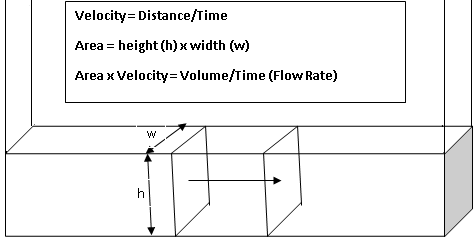
\includegraphics[scale=0.5]{ChannelFlow3}\\
$Q=V*A \implies Q = 1.5 \dfrac{ft}{sec}*(3*2)ft^2=\boxed{9\dfrac{ft^3}{sec}}$

\item Solution:\\
\vspace{0.25cm}
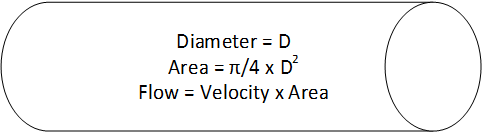
\includegraphics[scale=0.5]{PipeFlow}\\
$Q=V*A$\\
$\implies V=\dfrac{Q}{A} \implies V \Big(\dfrac{ft}{s}\Big)= \dfrac{\dfrac{500\cancel{gallon}}{\cancel{min}}*\dfrac{\cancelto{ft}{ft^3}*\dfrac{min}{60sec}}{7.48\cancel{gal}}}{0.785*\Big(\dfrac{8}{12}\Big)^2\cancelto{}{ft^2}}=\boxed{3.2ft/s}$

\item Solution:\\

\vspace{0.25cm}

The diameter of the pipe is 4 inches. Therefore, the radius is 2 inches. Convert the 2 inches to feet.
$
\begin{aligned}
&\dfrac{2}{12}=0.6667 \mathrm{ft} \\
&\mathrm{A}=\pi \times \mathrm{r}^{2} \\
&\mathrm{~A}=\pi \times(0.167 \mathrm{ft})^{2} \\
&\mathrm{~A}=\pi \times 0.028 \mathrm{ft}^{2} \\
&\mathrm{~A}=0.09 \mathrm{ft}^{2} \\
&\mathrm{Q}=\mathrm{V} \times \mathrm{A} \\
&\mathrm{Q}=1.5 \mathrm{ft} / \mathrm{sec} \times 0.09 \mathrm{ft}^{2} \\
&\mathrm{Q}=0.14 \mathrm{ft} / 3 \mathrm{sec}(\mathrm{cfs})
\end{aligned}
$



\vspace{1cm}
\end{enumerate}
\vspace{1cm}

\section*{Practice Problems - Unit Conversions}
Convert the following:\\
\begin{enumerate}
\item Convert 1000 $ft^3$ to cu. yards\\

\item Convert 10 gallons/min to $ft^3$/hr\\

\item Convert 100,000 $ft^3$ to acre-ft.\\

\item Find the flow in gpm when the total flow for the day is 65,000 gpd.

\item Find the flow in gpm when the flow is $1.3 \mathrm{cfs}$.

\item Find the flow in gpm when the flow is $0.25 \mathrm{cfs}$.

\item The flow rate through a filter is 4.25 MGD. What is this flow rate expressed as gpm?\\

\item After calibrating a chemical feed pump, you've determined that the maximum feed rate is $178 \mathrm{~mL} /$ minute. If this pump ran continuously, how many gallons will it pump in a full day?

\item A plant produces 2,000 cubic foot of water per hour. How many gallons of water is produced in an 8-hour shift?
\end{enumerate}
\textbf{Solution}
\begin{enumerate}
\item Solution:\\

$1000 \cancel{ft^3}*\dfrac{cu.yards}{27\cancel{ft^3}} = 37 cu.yards$

\item Solution:\\

\vspace{0.4cm}

$\dfrac{10 \enspace \cancel{\mathrm{gallons}}}{\cancel{\mathrm{min}}}*  \dfrac{\mathrm{ft}^3}{7.48 \cancel{\mathrm{gallons}}}  * \dfrac{60 \cancel{\mathrm{min}}}{\mathrm{hr}}   = \dfrac{80.2 \enspace \mathrm{ft}^3}{\mathrm{hr}}$

\vspace{0.4cm}


\item Solution:\\

\vspace{0.4cm}

$100,000 \cancel{ft^3} * \dfrac{acre-ft}{43,560 \cancel{ft^2-ft}} =  2.3 acre-ft$\\

\vspace{0.2cm}

\textbf{Note:} From the conversion table: acre = 43,560 $ft^2$\\
Thus, acre-ft  = 43,560 $ft^2$-ft or 43,560 $ft^3$\\

\vspace{0.4cm}

\item Solution:\\

\vspace{0.4cm}

$
\dfrac{65,000 \mathrm{gpd}}{1,440 \mathrm{~min} / \mathrm{day}}=45 \mathrm{gpm}
$

\vspace{0.4cm}

\item Solution:\\
$
1.3 \dfrac{\mathrm{cfs}}{1} \mathrm{x} \dfrac{448 \mathrm{gpm}}{1 \mathrm{cfs}}=582 \mathrm{gpm}
$

\vspace{0.4cm}

\item Solution:\\

\vspace{0.4cm}

$
0.25 \dfrac{\mathrm{cfs}}{1} \times \dfrac{448 \mathrm{gpm}}{1 \mathrm{cfs}}=112 \mathrm{gpm}
$

\vspace{0.4cm}

\item Solution:\\

\vspace{0.2cm}

$Flow rate, gpm=\dfrac{Flow \enspace rate, \enspace gpd}{1440 \enspace min/day}$\\

\vspace{0.2cm}

Note:  We are assuming that the filter operated uniformly over that 24 hour period.\\

\vspace{0.3cm}

$Flow rate, gpm=\dfrac{4.25 \enspace \dfrac{\cancel{MG}}{\cancel{day}} *1,000,000 \enspace \dfrac{gal}{\cancel{MG}}}{1440\dfrac{min}{\cancel{day}}}=\boxed{2,951 \enspace gpm}$


\item Solution:\\

\vspace{0.4cm}

$\dfrac{2000 \enspace \cancel{\mathrm{ft}^3}}{\cancel{hr}}*  \dfrac{7.48 \enspace{\mathrm{gallons}}}{\cancel{\mathrm{ft}^3}}  * \dfrac{60 \enspace \cancel{\mathrm{hr}}}{\mathrm{shift}}   = \boxed{\dfrac{119,680 \enspace \mathrm{gallons}}{\mathrm{shift}}}$

\vspace{0.4cm}
\end{enumerate}


\vspace{1cm}

\section*{Practice Problems - Concentration}
\begin{enumerate}
\item What is the concentration in mg/l of  4.5\% solution of that substance.

\item How many lbs of salt is needed to make 5 gallons of a 2,500mg/l solution

\end{enumerate}
\vspace{0.25cm}
\textbf{Solution}\\
\begin{enumerate}
\item 45,000 mg/l

\item Applying pounds formula:  lbs salt = $\dfrac{5}{1,000,000}*2,500*8.34=\boxed{0.14lbs}$
\end{enumerate}


\vspace{1cm}
\section*{Practice Problems - Density and Specific Gravity}
\begin{enumerate}

\item What is the specific gravity of a 1 ft$^3$ concrete block which weighs 145 lbs?

\item What is the specific gravity of a chlorine solution if 1 (one) gallon weighs 10.2lbs?

\item How much does each gallon of zinc orthophosphate weigh (pounds) if it has a specific gravity of 1.46?

\item How much does a 55 gallon drum of 25\% caustic soda weigh (pounds) if the specific gravity is 1.28?

\end{enumerate}

\section*{Practice Problems - Detention Time}
\begin{enumerate}
\item A flocculation basin is 7 ft deep, 15 ft wide, and 30 ft long. If the flow through the basin is 1.35 MGD, what is the detention time in minutes?

\item A tank has a diameter of 60 feet with an overflow depth at 44 feet. The current water level is 16 feet. Water is flowing into the tank at a rate of 250 gallons per minute. At this rate, how many days will it take to fill the tank to the overflow?

\item How long will it take to fill a 50 gallon hypochlorite tank if the flow is $5 \mathrm{gpm}$ ?

\item Find the detention time in a 45,000 gallon reservoir if the flow rate is $85 \mathrm{gpm}$.

\item If the fuel consumption to the boiler is 35 gallons per day. How many days will the 500 gallon tank last.

\item The sedimentation basin in a water plant contains 5,775 gallons. What is the detention time if the flow is $175 \mathrm{gpm}$.
\end{enumerate}

\textbf{Solution}\\
\begin{enumerate}
\item Solution:\\
\vspace{0.25cm}
\begin{tikzpicture}

\pgfmathsetmacro{\cubexx}{4}
\pgfmathsetmacro{\cubeyy}{1.5}
\pgfmathsetmacro{\cubezz}{2}
\pgfmathsetmacro{\cubex}{4}
\pgfmathsetmacro{\cubey}{0.5}
\pgfmathsetmacro{\cubez}{2}
\filldraw [fill=lightgray!20, draw=black] (0,-\cubey,0) -- ++(-\cubexx,0,0) -- ++(0,-\cubeyy,0) -- ++(\cubexx,0,0) -- cycle ;
\filldraw [fill=lightgray!20, draw=black] (0,-\cubey,0) -- ++(0,0,-\cubezz) -- ++(0,-\cubeyy,0) -- ++(0,0,\cubezz) -- cycle;
\filldraw [fill=lightgray!20, draw=black] (0,-\cubey,0) -- ++(0,0,-\cubezz) -- ++(0,-\cubeyy,0) -- ++(0,0,\cubezz) -- cycle;
\filldraw [fill=lightgray!20, draw=black] (0,-\cubey,0) -- ++(-\cubexx,0,0) -- ++(0,0,-\cubezz) -- ++(\cubexx,0,0) -- cycle;
%\draw (0,-0.5,0) -- ++(-\cubex,0,0) -- ++(0,-\cubey,-\cubez) -- ++(\cubex,0,0) -- cycle;
\draw (-\cubex,0,0) -- ++(0,0,-\cubez) -- ++(0,-\cubey,0) -- ++(0,0,\cubez) -- cycle;
\draw (0,-\cubey,0) -- ++(-\cubex,0,0) -- ++(0,0,-\cubez) -- ++(\cubex,0,0) -- cycle;




\filldraw [fill=white, draw=black] (0,0,0) -- ++(-\cubex,0,0) -- ++(0,-\cubey,0) -- ++(\cubex,0,0) -- cycle ;
\filldraw [fill=white, draw=black] (0,0,0) -- ++(0,0,-\cubez) -- ++(0,-\cubey,0) -- ++(0,0,\cubez) -- cycle;
\filldraw [fill=white, draw=black] (0,0,0) -- ++(0,0,-\cubez) -- ++(0,-\cubey,0) -- ++(0,0,\cubez) -- cycle;
\filldraw [fill=white, draw=black] (0,0,0) -- ++(-\cubex,0,0) -- ++(0,0,-\cubez) -- ++(\cubex,0,0) -- cycle;
%\draw (0,-0.5,0) -- ++(-\cubex,0,0) -- ++(0,0,-\cubez) -- ++(\cubex,0,0) -- cycle;
%\filldraw [fill=white, draw=black] (-\cubex,0,0) -- ++(0,0,-\cubez) -- ++(0,-\cubey,0) -- ++(0,0,\cubez) -- cycle;
%\filldraw [fill=white, draw=black] (0,-\cubey,0) -- ++(-\cubex,0,0) -- ++(0,0,-\cubez) -- ++(\cubex,0,0) -- cycle;

\draw [<->] (-4,-2.3) -- (0,-2.3) node [midway, below] {\scriptsize{30' long}};
\draw [<->] (1,-1.3) -- (1,.2) node [midway, below] {\hspace{2.2cm}\scriptsize{7' deep}};
%\draw [<->] (1,.8) -- (1,.2) node [midway, below] {\hspace{2.2cm}Text Y Axis};
\draw [<->] (1,-1.3) -- (0,-2.3) node [midway, below] {\hspace{1.7cm}\scriptsize{15' wide}};
\draw [->](-6,-1) -- (-4,-1) node [midway, above] {\hspace{0.5cm}\scriptsize{1.5 MGD}};
\draw [->](0.3,-1) -- (0.9,-1) node [midway, above] {};
\end{tikzpicture}\\

\vspace{0.4cm}
$
\mathrm{DT}=\dfrac{(30*15*7) \mathrm{ft^3}*7.48\dfrac{gal}{ft^3}}{1,350,000 \dfrac{\mathrm{gal}}{day}*\dfrac{\mathrm{day}}{1440\mathrm{min}}}=25 \mathrm{min}
$


\vspace{0.4cm}


\item Solution:\\

\vspace{0.4cm}
\begin{tikzpicture}[scale=1]
\node [draw, cylinder, cylinder uses custom fill, cylinder body fill=green!20, 
cylinder end fill=green!20, shape aspect=4, rotate=90, minimum width=3cm] (c1) at 
(0,1.8){};

\coordinate(dhtop) at ($(c1.after top)!-1*.1!(c1.before top)$);
\coordinate(dhbot) at ($(c1.before bottom)!-1*.1!(c1.after bottom)$);
\coordinate(dhlabel) at ($(dhtop)!.5!(dhbot)$);
%\draw[|-|] (dhbot)--(dhtop);
%\path (dhlabel) node[right, outer sep = 2pt] {$44'$};

\node [draw, cylinder, cylinder body fill=black!20, cylinder end fill=red!20, shape aspect=4, rotate=90, minimum height=4cm, minimum width=3cm] (c) {};

\coordinate(htop) at ($(c.before top)!-1*.1!(c.after top)$);
\coordinate(hbot) at ($(c.after bottom)!-1*.1!(c.before bottom)$);
\coordinate(hlabel) at ($(htop)!.5!(hbot)+(c.north)!.9!(c.center)$);

%\draw[|-|] (hbot)--(htop);
%\path (hlabel) node[left] {}; %Modify height label here


%\node [draw, cylinder, cylinder uses custom fill, cylinder body fill=black!20, 
%cylinder end fill=lightgray!20, shape aspect=4, rotate=90, minimum width=3cm] (c1) at 
%(0,3.8){};


\node [draw, cylinder, cylinder uses custom fill, cylinder body fill=black!20, 
cylinder end fill=lightgray!20, shape aspect=4, rotate=90, minimum width=3cm] (c1) at 
(0,-1.2){};

%\node [draw, cylinder, cylinder uses custom fill, cylinder body fill=blue!20, 
cylinder end fill=green!20, shape aspect=4, rotate=90, minimum width=3cm] (c1) at 
(0,0){};

%\coordinate (center) at ($(c.before top)!0.5!(c.after top)$);
%\filldraw (center) circle (1pt);
%
%\coordinate (rlabel) at ($(center) !0.5!(c.after top)$);
%\coordinate (rtop) at ($(center)!-1*.1!(c.after top)$);

%\coordinate (rend) at ($(c.mid east)!0.5!(c.after top)$);
%\draw[-, shorten >=-10] (center) -- (rend);
%\path (rend) node[outer sep = 5pt, left] {$r$};
\draw [<->] (-1.5,2.4) -- (1.5,2.4) node [midway, above=1mm] {\hspace{0.05cm}\scriptsize{Diameter=60'}};
%\draw [<->] (1.8,2.4) -- (1.8,1.9) node [midway, midway] {\hspace{2.4cm}\scriptsize{16' Freeboard}};
%\draw [<->] (1.8,1.9) -- (1.8,-0.7) node [midway, midway] {\hspace{2.4cm}\scriptsize{28' Fill}};
%\draw [<->] (1.8,-1.1) -- (1.8,-0.7) node [midway, midway] {\hspace{2.8cm}\scriptsize{16' Current Level}};
\draw (3.3,1.9) node{\scriptsize{Overflow level = 44'}};
\draw (3.22,-0.6) node{\scriptsize{Current level = 16'}};
\draw [<-] (1.5,-0.6) -- (2.2,-0.6);
\draw [<-] (1.5,1.9) -- (2.2,1.9);
\draw[thick,->](0,3.5)--(0,2.5) node [at start, above, black] (n){\scriptsize{250 gpm}};
\end{tikzpicture}

$\mathrm{Fill \enspace time}=\dfrac{Volume}{Flow}=\dfrac{0.785*60^2*(44-16)ft^3*\dfrac{7.48 gallons}{ft^3}}{250 \dfrac{gallons}{min}*\dfrac{1440 \enspace min}{day}}=1.6 \enspace days$
\vspace{0.4cm}

\item Solution:\\

\vspace{0.4cm}

$
\mathrm{DT}=\dfrac{50 \mathrm{gal}}{5 \mathrm{gal} / \mathrm{min}}=10 \mathrm{~min}
$

\vspace{0.4cm}

\item Solution:\\

\vspace{0.4cm}

$
\mathrm{DT}=\dfrac{45,000 \mathrm{gal}}{85 \mathrm{gal} / \mathrm{min}}=529 \mathrm{~min} \quad \text { or } \dfrac{529 \mathrm{~min}}{60 \mathrm{~min} / \mathrm{hr}}=8.8 \mathrm{hrs}
$
\vspace{0.4cm}

\item Solution:\\

\vspace{0.4cm}

$
\mathrm{DT}=\dfrac{500 \text { gal }}{35 \mathrm{gal} / \text { day }}=14.3 \text { days }
$
\vspace{0.4cm}

\item Solution:\\

\vspace{0.4cm}

$
\mathrm{DT}=\dfrac{5,775 \mathrm{gal}}{175 \mathrm{gal} / \mathrm{min}}=33 \mathrm{~min}
$

\end{enumerate}
\vspace{1cm}

\section*{Practice Problems - Pounds Formula}
\begin{enumerate}

\item A water treatment plant operates at the rate of 75 gallons per minute. They dose soda ash at
14 mg/l. How many pounds of soda ash will they use in a day?

\item A water treatment plant is producing 1.5 million gallons per day of potable water, and
uses 38 pounds of soda ash for pH adjustment. What is the dose of soda ash at that plant?

\item A water treatment plant produces 150,000 gallons of water every day. It uses an
average of 2 pounds of permanganate for iron and manganese removal. What is the dose of the
permanganate? 

\item A water treatment plant uses 8 pounds of chlorine daily and the dose is 17 mg/l. How
many gallons are they producing?

\item An operator mixes 40 lb of lime in a 100-gal tank containing 80 gal of water. What is the percent of lime in the slurry?

\item A treatment plant has a maximum output of $30 \mathrm{MGD}$ and doses ferric chloride at 75 $\mathrm{mg} / \mathrm{L}$. How many pounds of Ferric Chloride does the plant use in a day?\\

\item  A treatment plant uses 750 pounds of alum a day as it treats $15 \mathrm{MGD}$. What was the dose rate?\\


\item  A treatment plant operates at 1,500 gallons a minute and uses 500 pounds of alum a day. What is the alum dose?\\

\end{enumerate}

\textbf{Solution:}
\begin{enumerate}[1.]
\item Solution:\\

\begin{figure}[h]
\begin{tikzpicture}
    \newcommand{\R}{1.5}

\path[help lines,step=.2] (0,0) grid (16,3);
\path[help lines,line width=.6pt,step=1] (0,0) grid (16,3);
%\foreach \x in {0,1,2,3,4,5,6,7,8,9,10,11,12,13,14,15,16}
%\node[anchor=north] at (\x,0) {\x};
%\foreach \y in {0,1,2,3,4,5,6}
%\node[anchor=east] at (0,\y) {\y};
%-------------CIRCLE-----------------------------------
\draw[black,fill=gray!10] (8,3) circle (\R);
\draw[black, very thick, rotate=0](6.5,3) -- (9.5,3);
\draw (8,3.6) node[text width=3cm,align=center]
  {\scriptsize{lbs/day}};
\draw (7.1,2.5) node[text width=3cm,align=center]
  {\tiny{14 mg/l}};
\draw (8.9,2.5) node[text width=3cm,align=center]
  {\tiny{75 GPM}};
  \draw (8,2)node[text width=3cm,align=center]
  {\tiny{8.34}};
\draw[black, very thick, rotate=0](7.2,1.7) -- (8,3);
\draw[black, very thick, rotate=0](8.8,1.7) -- (8,3);
\end{tikzpicture}
\end{figure}
$\dfrac{\mathrm{lbs}}{\mathrm{day}}=\mathrm{Flow}\dfrac{{\mathrm{MG}}}{\mathrm{day}}* \mathrm{Concentration}\dfrac{\mathrm{mg}}{\mathrm{l}}*8.34$
\\
\vspace{0.2cm}
$\dfrac{\mathrm{lbs}}{\mathrm{day}}=75 \dfrac{\cancel{\mathrm{gallons}}}{\cancel{\mathrm{min}}}* 1440\dfrac{\cancel{\mathrm{min}}}{\mathrm{day}}*\dfrac{\mathrm{MG}}{1,000,000 \enspace \cancel{\mathrm{gallons}}}*250\dfrac{\mathrm{mg}}{\mathrm{l}}*8.34 = \boxed{225\dfrac{lbs}{day}}$
\vspace{0.2cm}
 \item Solution:\\
 \begin{figure}[h!]
\begin{tikzpicture}
    \newcommand{\R}{1.5}

\path[help lines,step=.2] (0,0) grid (16,3);
\path[help lines,line width=.6pt,step=1] (0,0) grid (16,3);
%\foreach \x in {0,1,2,3,4,5,6,7,8,9,10,11,12,13,14,15,16}
%\node[anchor=north] at (\x,0) {\x};
%\foreach \y in {0,1,2,3,4,5,6}
%\node[anchor=east] at (0,\y) {\y};
%-------------CIRCLE-----------------------------------
\draw[black,fill=gray!10] (8,3) circle (\R);
\draw[black, very thick, rotate=0](6.5,3) -- (9.5,3);
\draw (8,3.6) node[text width=3cm,align=center]
  {\scriptsize{38 lbs/day}};
\draw (7.1,2.5) node[text width=3cm,align=center]
  {\tiny{? mg/l}};
\draw (8.9,2.5) node[text width=3cm,align=center]
  {\tiny{1.5 MGD}};
  \draw (8,2)node[text width=3cm,align=center]
  {\tiny{8.34}};
\draw[black, very thick, rotate=0](7.2,1.7) -- (8,3);
\draw[black, very thick, rotate=0](8.8,1.7) -- (8,3);
\end{tikzpicture}
\end{figure}
$\dfrac{\mathrm{lbs}}{\mathrm{day}}=\mathrm{Flow}\dfrac{{\mathrm{MG}}}{\mathrm{day}}* \mathrm{Concentration}\dfrac{\mathrm{mg}}{\mathrm{l}}*8.34 \hspace{0.2cm} \implies \mathrm{Concentration}\dfrac{\mathrm{mg}}{\mathrm{l}}=\dfrac{ \dfrac{\mathrm{lbs}}{\mathrm{day}}}{\mathrm{Flow}\dfrac{{\mathrm{MG}}}{\mathrm{day}}*8.34}$
\vspace{0.2cm}
$\mathrm{Concentration}\dfrac{\mathrm{mg}}{\mathrm{l}}=\dfrac{ 38\dfrac{\mathrm{lbs}}{\mathrm{day}}}{1.5\dfrac{{\mathrm{MG}}}{\mathrm{day}}*8.34}=\boxed{3\dfrac{\mathrm{mg}}{\mathrm{l}}}$
\\
\vspace{0.2cm}



 \item Solution:\\
 \begin{figure}[h!]
\begin{tikzpicture}
    \newcommand{\R}{1.5}

\path[help lines,step=.2] (0,0) grid (16,3);
\path[help lines,line width=.6pt,step=1] (0,0) grid (16,3);
%\foreach \x in {0,1,2,3,4,5,6,7,8,9,10,11,12,13,14,15,16}
%\node[anchor=north] at (\x,0) {\x};
%\foreach \y in {0,1,2,3,4,5,6}
%\node[anchor=east] at (0,\y) {\y};
%-------------CIRCLE-----------------------------------
\draw[black,fill=gray!10] (8,3) circle (\R);
\draw[black, very thick, rotate=0](6.5,3) -- (9.5,3);
\draw (8,3.6) node[text width=3cm,align=center]
  {\scriptsize{38 lbs/day}};
\draw (7.1,2.5) node[text width=3cm,align=center]
  {\tiny{? mg/l}};
\draw (8.9,2.5) node[text width=3cm,align=center]
  {\tiny{1.5 MGD}};
  \draw (8,2)node[text width=3cm,align=center]
  {\tiny{8.34}};
\draw[black, very thick, rotate=0](7.2,1.7) -- (8,3);
\draw[black, very thick, rotate=0](8.8,1.7) -- (8,3);
\end{tikzpicture}
\end{figure}
$\dfrac{\mathrm{lbs}}{\mathrm{day}}=\mathrm{Flow}\dfrac{{\mathrm{MG}}}{\mathrm{day}}* \mathrm{Concentration}\dfrac{\mathrm{mg}}{\mathrm{l}}*8.34 \hspace{0.2cm} \implies \mathrm{Concentration}\dfrac{\mathrm{mg}}{\mathrm{l}}=\dfrac{ \dfrac{\mathrm{lbs}}{\mathrm{day}}}{\mathrm{Flow}\dfrac{{\mathrm{MG}}}{\mathrm{day}}*8.34}$
\vspace{0.2cm}
$\mathrm{Concentration}\dfrac{\mathrm{mg}}{\mathrm{l}}=
\dfrac{ 2\dfrac{\mathrm{lbs}}{\mathrm{day}}}
{\Bigg(150,000 \dfrac{\cancel{\mathrm{Gallons}}}
{\mathrm{day}}*
\dfrac{\mathrm{MG}}
{1,000,000 \cancel{\enspace \mathrm{Gallons}}}*8.34\Bigg)}
=\boxed{3\dfrac{\mathrm{mg}}{\mathrm{l}}}$
\\
\vspace{0.2cm}


 \item Solution:\\
 \begin{figure}[h!]
\begin{tikzpicture}
    \newcommand{\R}{1.5}

\path[help lines,step=.2] (0,0) grid (16,3);
\path[help lines,line width=.6pt,step=1] (0,0) grid (16,3);
%\foreach \x in {0,1,2,3,4,5,6,7,8,9,10,11,12,13,14,15,16}
%\node[anchor=north] at (\x,0) {\x};
%\foreach \y in {0,1,2,3,4,5,6}
%\node[anchor=east] at (0,\y) {\y};
%-------------CIRCLE-----------------------------------
\draw[black,fill=gray!10] (8,3) circle (\R);
\draw[black, very thick, rotate=0](6.5,3) -- (9.5,3);
\draw (8,3.6) node[text width=3cm,align=center]
  {\scriptsize{8 lbs/day}};
\draw (7.1,2.5) node[text width=3cm,align=center]
  {\tiny{17 mg/l}};
\draw (8.9,2.5) node[text width=3cm,align=center]
  {\tiny{? MGD}};
  \draw (8,2)node[text width=3cm,align=center]
  {\tiny{8.34}};
\draw[black, very thick, rotate=0](7.2,1.7) -- (8,3);
\draw[black, very thick, rotate=0](8.8,1.7) -- (8,3);
\end{tikzpicture}
\end{figure}
$\dfrac{\mathrm{lbs}}{\mathrm{day}}=\mathrm{Flow}\dfrac{{\mathrm{MG}}}{\mathrm{day}}* \mathrm{Concentration}\dfrac{\mathrm{mg}}{\mathrm{l}}*8.34 \hspace{0.2cm}$\\
\vspace{0.2cm}
$\implies \mathrm{Flow}\dfrac{{\mathrm{MG}}}{day}=\dfrac{ \dfrac{\mathrm{lbs}}{\mathrm{day}}}{\mathrm{Concentration}\dfrac{\mathrm{mg}}{\mathrm{l}}*8.34}=\dfrac{8 \dfrac{\mathrm{lbs}}{\mathrm{day}}}{17\dfrac{\mathrm{mg}}{\mathrm{l}}*8.34}=0.056425\dfrac{{\mathrm{MG}}}{day}$\\
\vspace{0.2cm}
$0.056425\dfrac{{\mathrm{MG}}}{day}*\dfrac{1,000,000 \enspace \mathrm{Gallons}}{\mathrm{MG}}=\boxed{56,425 \enspace \mathrm{Gallons}}$
\vspace{0.2cm}


 \item Solution:\\
 \begin{figure}[h!]
\begin{tikzpicture}
    \newcommand{\R}{1.5}

\path[help lines,step=.2] (0,0) grid (16,3);
\path[help lines,line width=.6pt,step=1] (0,0) grid (16,3);
%\foreach \x in {0,1,2,3,4,5,6,7,8,9,10,11,12,13,14,15,16}
%\node[anchor=north] at (\x,0) {\x};
%\foreach \y in {0,1,2,3,4,5,6}
%\node[anchor=east] at (0,\y) {\y};
%-------------CIRCLE-----------------------------------
\draw[black,fill=gray!10] (8,3) circle (\R);
\draw[black, very thick, rotate=0](6.5,3) -- (9.5,3);
\draw (8,3.6) node[text width=3cm,align=center]
  {\scriptsize{38 lbs/day}};
\draw (7.1,2.5) node[text width=3cm,align=center]
  {\tiny{? mg/l}};
\draw (8.9,2.5) node[text width=3cm,align=center]
  {\tiny{1.5 MGD}};
  \draw (8,2)node[text width=3cm,align=center]
  {\tiny{8.34}};
\draw[black, very thick, rotate=0](7.2,1.7) -- (8,3);
\draw[black, very thick, rotate=0](8.8,1.7) -- (8,3);
\end{tikzpicture}
\end{figure}
$\mathrm{lbs}=\mathrm{Volume}{\mathrm{(MG)}}* \mathrm{Concentration}\dfrac{\mathrm{mg}}{\mathrm{l}}*8.34 \hspace{0.2cm}$\\
\vspace{0.2cm}
$ \implies \mathrm{Concentration}\dfrac{\mathrm{mg}}{\mathrm{l}}=\dfrac{ \mathrm{lbs}}{\mathrm{Volume}\mathrm{(MG)}*8.34}=\dfrac{40 \enspace \mathrm{lbs}}{80 \enspace\mathrm{gallons}*\dfrac{\mathrm{MG}}{1,000,000 \enspace \cancel{\mathrm{gallons}}}*8.34}$
\vspace{0.2cm}

\vspace{0.2cm}


\end{enumerate}

%\mathrm{Concentration}\dfrac{\mathrm{mg}}{\mathrm{l}}
\vspace{1cm}
\section*{Practice Problems - Temperature Conversion}
\begin{enumerate}
\item Convert 22\degree{C} into degree Fahrenheit.
\item Convert 56\degree{C} into degree Celsius.
\end{enumerate}
\vspace{1cm}

\section*{Preliminary Treatment} \index{Preliminary Treatment}
\begin{enumerate}
\item On an average a 12.5 yd. load of grit is hauled to the landfill once every 20 days. Plant flow averages 12.5 MGD. Calculate the rate of grit collection in ft3/MG. \\

Correct Answer(s):\\
a. 1.4

\vspace{0.4cm}
\item A grit channel is 2 feet 4 inches wide. When wastewater is flowing 8 inches deep in this channel, the velocity is found to be 1.6 ft per second. Calculate flow in MGD. \\

a. 1.55 MGD \\
*b. 1.60 MGD \\
c. 1.90 MGD \\
d. 2.50 MGD 

\vspace{0.4cm}
\item A grit channel is 2 feet 4 inches wide. When wastewater is flowing 8 inches deep in this channel, the velocity is found to be 1.6 ft per second. Calculate flow in MGD. \\

a. 1.55 MGD \\
*b. 1.60 MGD \\
c. 1.90 MGD \\
d. 2.50 MGD 



\vspace{0.4cm}
\item At a wastewater treatment plant which receives a flow rate of 650,000 gallons per day, a total of 50 cubic feet of grit was removed for the month. Calculate the rate of grit removal assuming 30 days in a month.\\
Solution:\\
$Grit Removal\frac{ft^3}{MG}=50\frac{ft^3}{ \cancel{month}}*\frac{\cancel{month}}{30\cancel{days}}*\frac{\cancel{day}}{650,000\cancel{gal}}*1,000,000\frac{\cancel{gal}}{MG}=\boxed{2.6\frac{ft^3}{MG}}$

\vspace{0.4cm}
\item On an average a 12.5 yd. load of grit is hauled to the landfill once every 20 days. Plant flow averages 12.5 MGD. Calculate the rate of grit collection in ft$^3$/MG.\\
Solution:\\
$Grit Removal\Big(\frac{ft^3}{MG}\Big)=\frac{12.5\cancel{yd^3}}{ 20\cancel{days}}*\frac{27ft^3}{ \cancel{yd^3}}*\frac{\cancel{day}}{12.5MG}=\boxed{1.4\frac{ft^3}{MG}}$

\vspace{0.4cm}
\item On an average, 2 inches of grit is collected and removed every day in a 2.2 feet wide, 205 feet long grit channel.  Knowing the average flow through that grit channel is 10 MGD calculate the rate of grit collection in ft$^3$/MG\\
Solution:\\
Grit volume accumulated:  $\frac{2}{12}ft*(2.2*205)ft^2=\frac{75.16ft^3}{day}$
Grit Collection: $\frac{\frac{75.16ft^3}{\cancel{day}}}{\frac{10MG}{\cancel{day}}}=\boxed{7.5\frac{ft^3}{MG}}$ 

\vspace{0.4cm}
\item What is the grit production rate (cu. ft/MG) if 46 cu. ft of grit is removed every five days and the daily plant flow averages 2 MGD.\\

a. 12 cu. ft/MG \\
b. 23 cu. ft/MG \\
*c. 4.6 cu. ft/MG \\
d. 9.2 cu. ft/MG\\

Solution:\\
$Grit \enspace Production \enspace Rate\Big(\frac{ft^3}{MG}\Big)=\frac{46\cancel{ft^3}}{ 5\cancel{\enspace days}}*\frac{\cancel{day}}{2MG}=\boxed{4.6\frac{ft^3}{MG}}$


\vspace{0.4cm}
\item A grit chamber is 2 feet 4 inches wide. When wastewater is flowing 8 inches deep in this channel, the flow velocity is found to be 1.6 ft per second. Calculate flow in MGD.\\


Solution:\\
\vspace{0.3cm}
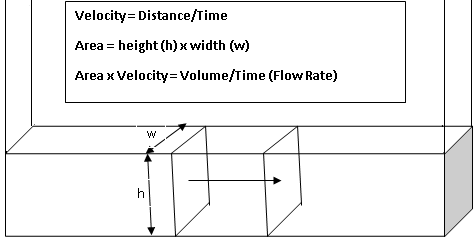
\includegraphics[scale=0.5]{ChannelFlow3}\\
$Q=V*A$\\
$Q=1.6\dfrac{ft}{s}*\Big(\dfrac{28}{12}*\dfrac{8}{12}\Big)ft^2=2.49\dfrac{ft^3}{s}$\\
$Q=2.49\dfrac{\cancel{ft^3}}{\cancel{s}}*\dfrac{(1440*60)\cancel{s}}{day}*7.48\dfrac{\cancel{gal}}{\cancel{ft^3}}\dfrac{MG}{\cancel{gal}}=\boxed{1.61MGD}$

\vspace{0.4cm}
\vspace{0.4cm}
\item  A steel bin is used to collect the daily accumulation of grit for disposal in a land fill. The bin is 8 ft long, 5.25 ft. wide, and 6 feet deep. When the bin is three-quarters full it is hauled away. This occurs on the average every 10 days. Average flow to the plant is \\3.75 MGD. What is the rate of grit collection in units of cubic feet per MG of flow?\\

Correct Answer(s):\\
a. 4.9


\vspace{0.4cm}
\item  A flow controlled grit chamber has two channels which are each 2.5 feet wide, and 20 feet long. Only one of these channels is currently in service and it receiving a flow of 4.5 MGD. The wastewater is flowing 1.5 feet deep in this channel. Calculate the velocity of this \\flow. Should we put the other channel in service?\\

Correct Answer(s): 

\vspace{0.4cm}
\item Calculate the flow, in gpd, that would pass through a grit chamber 2 feet wide, at a depth of 6 inches, with a velocity of 1 ft /sec.\\

Correct Answer(s):\\
a. 646272.0
\end{enumerate}



\section*{Primary Treatment} \index{Primary Treatment}
\begin{enumerate}
\item A clarifier has a TSS removal efficiency of 50\%.  If the influent TSS concentration is 220 mg/l, how many lbs/day of TSS are removed if the flow is 10 MGD.  Also, how many cu. ft of sludge is pumped if the sludge has a TS concentration of 5\%.\\
$lbs \enspace solids \enspace removed=(220*0.50)mg/l*10MGD*8.34=9,174lbs \enspace solids \enspace per \enspace day$
$$\frac{ft^3\enspace sludge}{day}= \frac{9,174 \enspace \cancel{lbs \enspace solids}}{day} * \frac{1 \enspace \cancel{lb \enspace sludge}}{0.05\enspace \cancel{lbs \enspace solids}}*\frac{\cancel{gal \enspace sludge}}{8.34\cancel{lb \enspace sludge}}*\frac{ft^3 \enspace sludge}{7.48 \enspace \cancel{gal}}=\boxed{2,941\frac{ft^3 \enspace sludge}{day}} $$

\item A community has a total flow of 15 MGD which is passed through a primary treatment plant which removes 60\% of the TSS and 35\% of the BOD. The average strength of the influent is 400 mg/l TSS and 275 mg/l BOD. If the total solids of the raw sludge is 5\%, how many cu. ft of sludge is pumped daily?
$lbs \enspace solids \enspace removed=(400*0.60)mg/l*15MGD*8.34=30,024lbs \enspace solids \enspace per \enspace day$
$$\frac{ft^3\enspace sludge}{day}= \frac{30,924 \enspace \cancel{lbs \enspace solids}}{day} * \frac{1 \enspace \cancel{lb \enspace sludge}}{0.05\enspace \cancel{lbs \enspace solids}}*\frac{\cancel{gal \enspace sludge}}{8.34\cancel{lb \enspace sludge}}*\frac{ft^3 \enspace sludge}{7.48 \enspace \cancel{gal}}=\boxed{9,626\frac{ft^3 \enspace sludge}{day}} $$

\item How many lbs of solids are removed daily by a primary clarifier treating a 6 MGD flow if the average influent TSS concentration is 300 mg/l and the clarifier TSS removal efficiency is 67\%?\\
As the removal efficiency is 67\%, 0.67 * 300 mg/l = 201 mg/l solids are removed.\\
The total lbs removed can be calculated using the lbs formula.\\
$ \frac{lbs \enspace solids}{day}= 6 MGD* 201  \frac{mg \enspace  SS}{l}*8.34=\boxed{10,058 \frac{lbs \enspace solids}{day}}$

\item Calculate the primary clarifier influent solids concentration if its outlet concentration is 60 mg/l and the known clarifier removal efficiency is 75\%?\\
$\frac{Actual \enspace  inlet \enspace (X)}{Actual \enspace outlet}=\frac{100}{100-Removal \enspace efficiency}$\\ 
$\frac{Actual \enspace  inlet \enspace (X)}{60}=\frac{100}{100-75}=4$\\
$\implies Actual \enspace inlet \enspace (X)=4*60 = \boxed{240 mg/l}$\\

\item A circular clarifier receives a flow of 11 MGD.  If the clarifier is 90 ft. in diameter and is 12 ft. deep, what is: a) the hydraulic/surface loading rate, b) weir overflow rate, and c) clarifier detention time in hours?\\
Solution:\\
a) Hydraulic/surface loading rate:\\
$Clarifier \enspace hydraulic \enspace loading \enspace 	\Big(\frac{gpd}{ft^2}\Big) ==\frac{\frac{11\cancel{MG}}{{day}}*\frac{10^6gal}{\cancel{MG}}}{0.785*90^2 ft^2}=\boxed{1,730gpd/ft^2}$\\
b) Weir overflow rate:\\ 
$Weir \enspace overflow \enspace rate \Big(\frac{gpd}{ft}\Big) =\frac{\frac{11\cancel{MG}}{{day}}*\frac{10^6gal}{\cancel{MG}}}{3.14*90 ft}=\boxed{38,924gpd/ft}$\\
c) Clarifier detention time:\\
$Clarifier \enspace detention \enspace time \enspace (hr) = 	\frac{ Clarifier \enspace volume (cu.ft \enspace or \enspace gal)}{Influent \enspace flow \enspace (cu.ft \enspace or \enspace gal)/hr)}$\\
$Clarifier \enspace detention \enspace time \enspace (hr) = 	\frac{(0.785*90^2*15)\cancel{ft^3}}{\frac{11\cancel{MG}}{\cancel{day}}*\frac{10^6\cancel{gal}}{\cancel{MG}}*\frac{\cancel{ft^3}}{7.48\cancel{gal}}*\frac{\cancel{day}}{24hrs}}=\boxed{2hrs}$\\
\vspace{1cm}
\item A clarifier has a TSS removal efficiency of 50\%.  If the influent TSS concentration is 220 mg/l, how many lbs/day of TSS are removed if the flow is 10 MGD.  Also, how many cu. ft of sludge is pumped if the sludge has a TS concentration of 5\%.\\
Solution:\\
$lbs \enspace solids \enspace removed=(220*0.50)mg/l*10MGD*8.34=9,174lbs \enspace solids \enspace per \enspace day$
$$\frac{ft^3\enspace sludge}{day}= \frac{9,174 \enspace \cancel{lbs \enspace solids}}{day} * \frac{1 \enspace \cancel{lb \enspace sludge}}{0.05\enspace \cancel{lbs \enspace solids}}*\frac{\cancel{gal \enspace sludge}}{8.34\cancel{lb \enspace sludge}}*\frac{ft^3 \enspace sludge}{7.48 \enspace \cancel{gal}}=\boxed{2,941\frac{ft^3 \enspace sludge}{day}} $$

\item If a clarifier has a capacity of 0.25 MG, what is the detention time in hours if it receives a flow of 3 MGD\\
Solution:\\
$Clarifier \enspace detention \enspace time \enspace (hr) = 	\frac{ Clarifier \enspace volume (MG)}{Influent \enspace flow \enspace (MG/hr)}$\\
\vspace{0.25cm}
$Clarifier \enspace detention \enspace time \enspace (hr) = 	\frac{0.25\cancel{MG}}{\frac{3\cancel{MG}}{\cancel{day}}*\frac{\cancel{day}}{24hrs}}=\boxed{2hrs}$\\

\item If a clarifier has a capacity of 0.25 MG, what is the detention time in hours if it receives a flow of 3 MGD\\
Solution:\\
$Clarifier \enspace detention \enspace time \enspace (hr) = 	\frac{ Clarifier \enspace volume (MG)}{Influent \enspace flow \enspace (MG/hr)}$\\
\vspace{0.25cm}
$Clarifier \enspace detention \enspace time \enspace (hr) = 	\frac{0.25\cancel{MG}}{\frac{3\cancel{MG}}{\cancel{day}}*\frac{\cancel{day}}{24hrs}}=\boxed{2hrs}$\\


\item At a 2.5 MGD wastewater treatment plant the primary clarifier has a detention time of 2 hours. How many gallons does this clarifier hold?\\

Solution:\\
\vspace{0.2cm}
$Clarifier \enspace detention \enspace time \enspace (hr) = 	\frac{ Clarifier \enspace volume (gal)}{Influent \enspace flow \enspace (gal/hr)}$\\
\vspace{0.2cm}
$ \implies Clarifier \enspace volume (gal)=Clarifier \enspace detention \enspace time \enspace (hr)*Influent \enspace flow \enspace (gal/hr)$\\
\vspace{0.2cm}
$ \implies Clarifier \enspace volume (gal)= \Big(2 \enspace hrs\Big)*\Big(2.5*10^6 \enspace \frac{gal}{day}*\frac{day}{24 \enspace hrs}\Big)=\boxed{208,333 \enspace gals}$\\


\item What is the surface loading rate (gal/(day-sq.ft) of a 15 MGD flow in a 105 ft diameter primary sedimentation tank operating at water depth of 20 ft.\\
\vspace{0.25cm}
Solution:\\
\vspace{0.25cm}
$Clarifier \enspace hydraulic \enspace loading \enspace 	\Big(\dfrac{gpd}{ft^2}\Big) =\dfrac{\dfrac{15\cancel{MG}}{{day}}*\dfrac{10^6gal}{\cancel{MG}}}{0.785*105^2 ft^2}=\boxed{1,733gpd/ft^2}$\\

\item If a 90 ft diameter primary clarifier operating at water depth of 20 ft is treating a 12MGD flow, calculate the surface loading rate (gal/(day-sq.ft).\\
Solution:\\
$Clarifier \enspace hydraulic \enspace loading \enspace 	\Big(\dfrac{gpd}{ft^2}\Big) =\dfrac{\dfrac{12\cancel{MG}}{{day}}*\dfrac{10^6gal}{\cancel{MG}}}{0.785*90^2 ft^2}=\boxed{1,887gpd/ft^2}$\\


\vspace{0.25cm}
\item What is the weir overflow rate (gpd/ft) when treating a 15 MGD flow in a 105 ft diameter primary sedimentation tank operating at water depth of 20 ft.\\
\vspace{0.25cm}
Solution:\\
\vspace{0.25cm}
$Clarifier \enspace detention \enspace time \enspace (hr) = 	\dfrac{(0.785*105^2*20)\cancel{ft^3}}{\dfrac{15\cancel{MG}}{\cancel{day}}*\dfrac{10^6\cancel{gal}}{\cancel{MG}}*\dfrac{\cancel{ft^3}}{7.48\cancel{gal}}*\dfrac{\cancel{day}}{24hrs}}=\boxed{2.1hrs}$\\

\item A circular clarifier receives a flow of 3.2 MGD. If the diameter is 70 ft, what is the weir overflow rate?\\
Solution:\\
$Weir \enspace overflow \enspace rate \Big(\dfrac{gpd}{ft}\Big) =\dfrac{\dfrac{3.2\cancel{MG}}{{day}}*\dfrac{10^6gal}{\cancel{MG}}}{3.14*70 ft}=\boxed{14,559gpd/ft}$\\ 


\vspace{0.25cm}
\item How many lbs/day of solids are removed in a clarifier treating a 6 MGD flow if the average inlet concentration is 320 mg/l and its average outlet concentration is 80 mg/l\\
\vspace{0.25cm}
Solution:\\
\vspace{0.25cm}
Applying pounds formula:\\
$\frac{lbs \enspace solids \enspace removed}{day}=6MGD*(320-80)\frac{mg}{l}*8.34=\boxed{120,096\frac{lbs \enspace solids}{day}}$

\vspace{0.25cm}
\item At a 2.5 MGD wastewater treatment plant the primary clarifier has a detention time of 2 hours. How many gallons does this clarifier hold?\\

\item  What is the detention time (hrs) in a 105' diameter primary sedimentation tank operating at water depth of 20' when treating a 15 MGD flow (Ans: 2.1)\\

\item  What is the surface loading rate (gal/(day-sq.ft) of a 15 MGD flow in a 105 ft diameter primary sedimentation tank operating at water depth of 20 ft. (Ans: 1,733)\\


\item  What is the weir overflow rate (gpd/ft) when treating a 15 MGD flow in a 105 ft diameter primary sedimentation tank operating at water depth of 20 ft. (Ans: 45,496)\\


\item  A circular clarifier receives a flow of 3.2 MGD. If the diameter is 70 ft, what is the weir overflow rate? (Ans: 14,559)\\


\item  A clarifier has an influent suspended solids concentration of 420 mg/l. If the suspended solids efficiency is 62\%, how many mg/l suspended solids are removed? (Ans: 260)\\


\item  Given the following for a primary sedimentation tank:\\
TSS removal efficiency = 63\%\\
Effluent TSS concentration = 95 mg/l\\
Calculate the influent TSS concentration (mg/l)\\
(Ans: 257)\\

\item  What is the clarifier influent TSS if its outlet concentration is 60 mg/l and the known clarifier removal efficiency is 75\%? \\


*a. 240 mg/l \\
b. 300 mg/l \\
c. 80 mg/l \\
d. 120 mg/l \\


\item  What is the clarifier removal efficiency if the inlet and outlet concentrations are 300 mg/l and 60 mg/l respectively?\\

a. 20\% \\
b. 30\% \\
*c. 80\% \\
d. 72\% \\


\item  A rectangular sedimentation tank is 85 feet long, 35 feet wide, and 14 feet deep including 3 feet of freeboard. Flow to this tank is 2.3 MGD. Calculate the surface loading to this tank in gpd per ft2.\\

a. 318 gpd/ft2 \\
*b. 773 gpd/ft2 \\
c. 845 gpd/ft2 \\
d. 1932 gpd/ft2 \\


\item  What is the detention time in a 40 ft diameter primary clarifier operating with a 12 ft water depth, when treating a 1.5 MGD flow?\\

a. 0.24 hours \\
b. 0.60 hours \\
*c. 1.8 hours \\
d. 2.3 hours \\
e. 11.0 hours \\


\item  How many lbs/day of solids are removed in a clarifier treating a 6 MGD flow if the average inlet concentration is 320 mg/l and its average outlet concentration is 80 mg/l\\

a. 16,000 lbs/day \\
*b. 1,210 lbs/day \\
c. 4,000 lbs/day \\
d. 9,000 lbs/day \\


\item  At a 5 MGD wastewater flow, a primary clarifier has a detention time of 1 hour. How many gallons does this clarifier hold?\\

a. 104,000 gallons \\
*b. 208,000 gallons \\
c. 250,000 gallons \\
d. 500,000 gallons \\
e. 5,000,000 gallons \\


\item  Percent efficiency of total solids or BOD removal is calculated using the following formula:  (In-Out*100)/(In-(In*Out))\\

a. True \\
*b. False \\


\item  The only function of flights in a rectangular sedimentation tank is to push the settled sludge towards the hopper\\

a. True \\
*b. False

\item  A settling basin has a length of 60 ft., width of 20 ft., and depth of 12 ft.  At a flow rate of 60 mgd, what is the retention time of this basin? \\

a. 15 minutes. \\
b. 30 minutes. \\
*c. 1.1 hours. \\
d. 2.3 hours. \\


\item  Calculate the detention time for a sedimentation tank that is 48 feet wide, 210 feet long and 9 feet deep with a flow of 5 MGD. \\

*a. 3.25 hours. \\
b. 3.63 hours. \\
c. 5.65 hours. \\
d. 5.82 hours. \\


\item  Calculate the weir loading for a sedimentation tank that has an outlet weir 480 ft. long and a flow of 5 MGD. \\

a. 9220 gpd/ft. \\
b. 9600 gpd/ft. \\
c. 9920 gpd/ft. \\
*d. 10,420 gpd/ft. \\


\item  If a primary clarifier consistently operates at 30 \% efficiency and produces an effluent which averages 140 mg/l BOD, what is the influent BOD? \\

a. 100 mg/l \\
b. 125 mg/l \\
c. 175 mg/l \\
*d. 200 mg/l \\
e. 225 mg/l \\


\item  At a 2.5 MGD wastewater treatment plant the primary clarifier has a detention time of 2 hours. How many gallons does this clarifier hold? \\

a. 104,000 gallons \\
*b. 208,000 gallons \\
c. 250,000 gallons \\
d. 500,000 gallons \\
e. 5,000,000 gallons \\


\item  A 3.1 MGD flow  with a 190 mg/l TSS concentration is treated in a primary clarifier which averages 55\% removal efficiency.  Calculate the pounds/day TSS in the primary effluent. \\

a. 2445 lbs/day \\
*b. 2211 lbs/day \\
c. 3800 lbs/day \\
d. 4200 lbs/day \\


\item  A 75 ft long, 25 ft wide and 10 ft deep sedimentation basin receives a flow of 1.6 MGD.  What is the detention time in hours. \\

a. 7 hrs \\
b. 1.7 hrs \\
*c. 2.1 hrs \\
d. 4 hrs \\


\item  A sludge pump is set to pump 5 minutes each hour. It pumps at the rate of 35 gpm. How many gallons of sludge are pumped each day? \\

a. 120 gpd \\
b. 175 gpd \\
c. 840 gpd \\
*d. 4200 gpd \\


\item  A primary clarifier has an influent suspended solids concentration of 250 mg/l. If the suspended solids  removal efficiency is 60\%, what is the primary effluent suspended solids concentration \\

a. 10 mg/l \\
*b. 100 mg/l \\
c. 50 mg/l \\
d. 150 mg/L \\


\item  A treatment plant receives a flow of 3.5 MGD.  If the clarifier is 100 ft. long, 30 ft. wide, and 15 ft. deep, what is the surface loading rate? \\

a. 78 gal/ft/day \\
b. 700 gal/ft/day \\
*c. 1,170 gal/ft/day \\
d. 1,500 gal/ft/day \\
e. 4,500 gal/ft /day \\


\item  A settling basin has a length of 60 ft, width of 20 ft, and depth of 12 ft At a flow rate of 60 MGD, what is the detention time of this basin? \\

a. 15 minutes \\
b. 30 minutes \\
*c. 1.1 hours \\
d. 2.3 hours \\


\item  If a clarifier has a capacity of 0.25 MG, what is the detention time in hours if it receives a flow of 3 MGD \\

a. 1.8 hrs \\
*b. 2.0 hrs \\
c. 2.25 hrs \\
d. 2.50 hrs \\
e. 3.00 \\
\end{enumerate}

\vspace{0.25cm}
Solution:\\
\vspace{0.25cm}
$Clarifier \enspace detention \enspace time \enspace (hr) = 	\frac{ Clarifier \enspace volume (gal)}{Influent \enspace flow \enspace (gal/hr)}$\\
\vspace{0.3cm}
$\implies Clarifier \enspace volume (gal)= Clarifier \enspace detention \enspace time \enspace (hr) * Influent \enspace flow \enspace (gal/hr)$\\
\vspace{0.3cm}
$\implies Clarifier \enspace volume (gal)= 2 hrs * 2,500,000\frac{gal}{day}*\frac{day}{24 \enspace hrs}=\boxed{208,333 gal}$\\




\section*{Trickling Filter} \index{Trickling Filter}
\begin{enumerate}
\item The influent to a trickling filter plant is 200 mg/l and the effluent BOD is 20 mg/l.  What is the BOD removal efficiency (%)? (Ans: 90)\\
 \item The flow to a trickling filter is 1.33 MGD. If the primary effluent has a BOD concentration of231 mg/land the trickling filter effluent has a BOD concentration of 83 mg/l, how many pounds of BOD are removed? (Ans: 1642 lbs/day)\\
 \item  A 80-ft diameter trickling filter with a media depth of 7 ft receives a flow of 2,180,000 gpd. If the BOD concentration of the primary effluent is 139 mg/l, what is the organic loading on the trickling filter in lbs BOD/day/1000 cu ft? (Ans: 72 lbs/day-1000 ft3)\\
 \item  A standard-rate filter, 90 ft in diameter, treats a primary effluent flow of 540,000 gpd. If the recirculated flow to the trickling filter is 120,000 gpd, what is the hydraulic loading rate on the filter in gpd/sq ft? (Ans: 104)\\
\item  A 90 feet diameter trickling filter treats a 540,000 gpd primary effluent flow.  If the recirculated flow to the trickling filter is 120,000 gpd, what is the hydraulic loading on the trickling filter in gpd/ft2.\\

 *a. 104 gpd/ft2 \\
 b. 2 gpd/ft2 \\
 c. 3 gpd/ft2 \\
 d. 4 gpd/ft2 \\


\item  A trickling filter plant operating at a recirculation ratio of 1 receives a raw wastewater flow of 2 MGD.  This means that the flow being applied to the filter would be: \\

 *a. 4mgd. \\
 b. 1mgd \\
 c. 3mgd \\
 d. 2mgd \\
 e. 6mgd \\


\item  What is the hydraulic loading of a trickling filter with a 100-foot diameter, if it receives a flow of 4.0 MGD? \\

 a. 480 GPD/ft2 \\
 *b. 510 GPD/ft2 \\
 c. 540 GPD/ft2 \\
 d. 570 GPD/ft2 \\
 e. 600 GPD/ft2 \\


\item  A 12 MGD primary clarifier effluent flow is fed to a trickling filter. If the total flow to the trickling filter including the recirculated flow is 17 MGD, what is the recirculation ratio? \\ (Ans: 0.42)

\item  A trickling filter 100  ft. in diameter and 6 ft. deep receives a flow of 0.5 mgd with  a BOD of 150 mg/l.  What is the BOD loading in pounds per day per 1000 cubic feet of filter media? \\

 a. 11.9. \\
 *b. 13.3. \\
 c. 26.8. \\
 d. 133. \\


\item  Calculate the organic load in lbs of BOD/day/1000 cu. ft. for a trickling filter 50 ft in diameter and eight (8) ft deep.  Given a flow of 250,000 gpd, and a 150 mg/l BOD concentration of the primary effluent feed to the trickling filter. \\

 a. 2 lbs/day/1000 cu. ft. \\
 b. 5 lbs/day/1000 cu. ft. \\
 *c. 20 lbs/day/1000 cu. ft. \\
 d. 50 Ibs/day/1000 cu. ft. \\


\item  Calculate the pounds of BOD per day entering the trickling filter.\\
 DATA: Raw wastewater flow is 1.5 MGD.\\
 Raw wastewater BOD is 150 mg/l.\\
 There is a 30% reduction in BOD across the primary clarifiers.\\
 *a. 1600 lbs/day \\
 b. 880 lbs/day \\
 c. 870 lbs/day \\
 d. 560 lbs/day \\


\item  A trickling filter wastewater treatment plant receives a flow 1.95 MGD. Calculate the organic loading to this plant if it has a 135 ft diameter trickling filter with a 5 foot media depth and has a primary effluent BOD concentration of 110 mg/l. \\

 a. 0.5 lbs BOD/1,000 ft³/day. \\
 b. 2.7 lbs BOD/1,000 ft³/day. \\
 *c. 25 lbs BOD/1,000 ft³/day. \\
 d. 39 lbs BOD/1,000 ft³/day. \\
 e. 44 lbs BOD/1,000 ft³/day. \\


\item  At a 2.1 MGD wastewater treatment plant the influent suspended solids concentration to the primary clarifier is 240 mg/l.  The primary sludge contains 3.2% TS and the primary effluent a suspended solids concentration of 125 mg/l.  How many\\
 gallons of primary sludge should be pumped per day? \\

 a. 63,000 gal/day · \\
 b. 32,200 gal/day \\
 c. 8,200 gal/day \\
 *d. 7,550 gal/day \\


\item  Calculate the pounds of BOD per day entering the trickling filter\\
 DATA:\\
 Raw wastewater flow is 15 MGD\\
 Raw wastewater BOD is 150 mg/l\\
 There is a 30% reduction in BOD across the primary clarifiers \\

 a. 560 lbs/day \\
 b. 870 1 bs/ day \\
 c. 880 1 bs /day \\
 *d. 1600 lbs/day \\


\item  Calculate the organic load in lbs of BOD/day/1000 cu ft for a trickling filter 50 ft in diameter and 8 feet deep, a BOD design loading of 50 lbs/day/1000 cu ft, a flow of 250,000 gpd, and a primary effluent BOD to filter of 150 mg/l \\

 a. 2 lbs/day/1000 cu ft \\
 b. 5 lbs/day/1000 cu ft \\
 *c. 20 lbs/day/1000 cu ft \\
 d. 50 lbs/day/1000 cu ft \\

\item  What is the trickling filter hydraulic loading if the influent flow is 3 MGD and the recirculation rate is 4:1? \\

 a. 3 mgd \\
 b. 6mgd \\
 c. 9mgd \\
 d. 12mgd \\
 *e. 15 mgd \\
 f. None of the above \\


\item  Calculate the organic load in lbs of BOD/day/1000 cu. ft. for a trickling filter 50 ft in diameter and eight (8) ft deep.  Given a flow of 250,000 gpd, and a 150 mg/l BOD concentration of the primary effluent feed to the trickling filter. \\

 a. 2 lbs/day/1000 cu. ft. \\
 b. 5 lbs/day/1000 cu. ft. \\
 *c. 20 lbs/day/1000 cu. ft. \\
 d. 50 Ibs/day/1000 cu. ft. \\

\item  The desired trickling filter recirculation ratio is 1.4.  If the primary effluent flow is 4.4 MGD what is the trickling filter effluent flow that needs to be recirculated. \\ (Ans: 6.2)


\end{enumerate}

\section*{Stabilization Ponds}\index{Stabilization Ponds}

\begin{enumerate}

\item  A 40 acre pond receives a 0.6 MGD flow.  If the pond is operated at a depth of 4ft, what is the detention time (days) of this pond. (Ans: 87)\\


\item  The flow to a pond is 750 gpm. The pond width is 200 ft and length is 450 ft. If the BOD in the pond influent is 240mg/l, what is the organic loading to this pond in lbs-BOD/day/acre? (Ans: 1046)\\


\item  Calculate the depth the liquid level must be lowered in the fall below the normal 3-foot depth to prepare for winter and provide 180 day storage.
DATA: Wastewater stabilization ponds total area of 13.8 acres (600,000 sq. ft.)
Average winter wastewater flow to the ponds is 100,000 gpd.  Maximum liquid storage depth is 5 feet.
(Assume no loss of liquid by percolation or evaporation and that the ponds will fill to the maximum storage level of 5 feet.) \\


a. 0.1 ft. \\

b. 1.0 ft. \\

*c. 2.0 ft. \\

d. 4.0 ft. \\

\item  Compute the lagoon's detention time (days)
DATA: Surface area= 6.0 acres
Average depth= 3.0 feet
Average evaporation exceeds precipitation by 0.4 in/day
Average daily flow (influent)= 0.25 MGD
1 acre (area)= 43,560 sq ft
1 cu ft contains 7.5 gal \\


a. 24 \\

*b. 32 \\

c. 37 \\

d. None of the above \\

\item  A pond is 600 ft. long and 150 ft. wide. If the pond is 6 ft. deep, what is the volume in  acre ft? (Ans: 13.9)\\

\item  A wastewater pond has a detention time of 30 days and is operated at a pond depth of 4 ft.  What is the hydraulic loading on the pond? \\


a. 7.5 in/day \\

*b. 1.6 in/day \\

c. 0.63 in/day \\

d. 0.41 in.day \\

e. 013 in/day \\


\item  The volume of an aerated pond is 700,000 cubic feet.  Flow to the pond averages .050 MGD. How many days detention time does the pond provide? \\


a. 10.5 days. \\

b. 14 days. \\

*c. 105 days. \\

d. 140 days. \\



\item  Assume a community of 1,100 people has a lagoon. The flow averages 80,000 gallons per day. The flow is 

a. 14 gallons per capita. \\
*b. 72 gallons per capita. \\
c. 80 gallons per capita. \\
d. 140 gallons per capita. 

\item  What is the organic loading on a lagoon (lbs./day/acre) if the influent BOD averages 164 mg/l and the flow averages 0.67 MGD. The lagoon has two (2) identical square cells with each side of 800 ft. 

a. 29 lbs./ac. \\
b. 23 lbs./ac. \\
*c. 31 lbs./ac. \\
d. 52 lbs./ac. \\


\item A stabilization pond is 1100 ft. long, 600 ft wide, and is operated at a depth of 5 ft. It receives a flow of 500,000 gpd and which has an influent BOD of 185mg/l.  Using this information do the following:
\begin{enumerate}
\item Convert the flow to the pond in units of acre-ft/day \textbf{(Ans. 1.53 acre-ft/day)}
\item Find the area of this pond in units of acres. \textbf{(Ans. 540,000 ft3 and 13.9 acre-ft)}\textbf{(Ans. 15.2 acres)}
\item Find the volume of pond in units of acre-feet. \textbf{(Ans. 75.8 acre-ft)}
\item Calculate the pond detention time in days. \textbf{(Ans. 44.9)}
\item Calculate the hydraulic loading to the pond in units of inches per day. \textbf{(Ans. 1.2 in/day)}
\item Calculate the organic loading to the pond (lbs of BOD/day/acre) \textbf{(Ans. 50.8 lbs BOD/day-acre)}
\end{enumerate}


Solution:\\
\begin{enumerate}
\item $\dfrac{500,000gal}{day}*\dfrac{ft^3}{7.48gal}*\dfrac{acre-ft}{43,560ft^3}=\boxed{1.53\dfrac{acre-ft}{day}}$
\item $(1,100*600)ft^2*\dfrac{acres}{43,560 ft^2}=\boxed{15.2acres}$
\item $(1,100*600*5)ft^3*\dfrac{acres-ft}{43,560 ft^3}=\boxed{75.8 acre-ft}$
\item $DT=\dfrac{volume}{flow}=(1,100*600*5)ft^3*\dfrac{1}{500,000\d
frac{gal}{day}}\dfrac{7.48gal}{ft^3}=\boxed{49.4days}$
\item $Pond \enspace hydraulic \enspace loading \enspace rate \Bigg[\dfrac{in}{day}\Bigg]=\dfrac{Pond \enspace depth \enspace (in)}{Pond \enspace detention  \enspace time \enspace \dfrac{Volume}{Flow}}=\dfrac{5*12in}{49.4}=\boxed{1.2\dfrac{in}{day}}$ \\
\item $Organic \enspace loading=\dfrac{lbs \enspace BOD \enspace per \enspace day}{area \enspace (acres)}$\\
$\implies \dfrac{0.5MGD \enspace * \enspace 185mg/l \enspace * \enspace 8.34}{1,100*600ft^2}*\dfrac{43,560ft^2}{acre}=\boxed{\dfrac{50.9lbs \enspace BOD}{day-acre}}$
\end{enumerate}

\item What is the surface area of a pond that is 4 feet deep, if it holds 30 million gallons?\\

Solution:\\
$Pond \enspace Volume= Surface \enspace Area*Depth \implies 30MG=Surface \enspace Area*4ft$\\
$ \implies Surface \enspace Area \enspace (acres)=\dfrac{30MG*3.069\dfrac{acre-ft}{MG}}{4ft}=\boxed{23 \enspace acre}$
\item The influent flow to a pond is 10,000 gallons/hour with a suspended solids concentration of 142mg/l in the raw wastewater.  How many lbs of suspended solids are sent to the pond daily?
\\
Solution:\\
$\dfrac{lbs SS}{day}=10000\dfrac{gal}{hr}*\dfrac{24hrs}{day}*\dfrac{MG}{1000000gal}*142\dfrac{mg}{l}*8.34=\boxed{284\dfrac{lbs \enspace SS}{day}}$
\item A pond is 260 ft. long and 80 ft. wide. What is the area of this pond in acres?\\ 
Solution:\\
$(260*80)ft^2*\dfrac{acre}{43,560ft^2}=\boxed{0.48acre}$
\item A pond has a volume of 1,800,000 $ft^3$. If the flow to the pond is 425 gpm, what is the pond detention time in days?
\\
Solution:\\
$DT=\dfrac{volume}{flow}=1,800,000ft^3*\dfrac{1}{425\dfrac{gal}{min}}*\dfrac{day}{1440min}*\dfrac{7.48gal}{ft^3}=\boxed{22days}$
\item Find pond hydraulic loading in inches/day when the depth of the pond is 6 ft. and the detention time is 30 days.\\
Solution:\\

$Hydraulic \enspace Loading \enspace (HL)=\dfrac{flow}{area}$\\
$Detention \enspace time \enspace (DT)=\dfrac{vol}{flow} \implies flow=\dfrac{vol}{DT} $\\
Substituting \enspace for \enspace flow \enspace in \enspace the HL \enspace formula above:\\
$HL=\dfrac{\dfrac{vol}{DT}}{area}\enspace or \enspace \dfrac{vol}{area*DT} \enspace \implies \boxed{HL=\dfrac{pond \enspace depth}{DT}} \enspace as \enspace \dfrac{vol}{area}=pond \enspace depth$\\

$Pond \enspace hydraulic \enspace loading \enspace rate=\dfrac{Pond \enspace depth \enspace (in)}{Pond \enspace detention  \enspace time \enspace \dfrac{Volume}{Flow}}=\dfrac{6*12 \enspace inches}{30 \enspace days}=\boxed{\dfrac{2.4in}{day}}$\\
\vspace{0.25cm}




\item The flow to a pond is 7.2MGD. If the pond diameter is 350 ft and the BOD in the pond influent is 170mg/l, what is the organic loading to this pond in lbs BOD/day/acre?
\\
Solution:\\
$Organic \enspace loading=\dfrac{lbs \enspace BOD \enspace per \enspace day}{area \enspace (acres)}=\dfrac{7.2MGD \enspace * \enspace 170mg/l \enspace * \enspace 8.34}{0.785*350^2ft^2}*\dfrac{43,560ft^2}{acre}=\boxed{\dfrac{4,624lbs \enspace BOD}{day-acre}}$

\item The flow to a pond is 750,000 gpd. If the pond diameter is 100 ft and the BOD in the pond influent is 300 mg/l, what is the organic loading to this pond in lbs BOD/day/acre? \textbf{(Ans. 10,412 lbs BOD/day-acre)}
\\
Solution:\\
$Organic \enspace loading=\dfrac{lbs \enspace BOD \enspace per \enspace day}{area \enspace (acres)}=\dfrac{0.75MGD \enspace * \enspace 300mg/l \enspace * \enspace 8.34}{0.785*100^2ft^2}*\dfrac{43,560ft^2}{acre}=\boxed{\dfrac{10,413lbs \enspace BOD}{day-acre}}$

\item A 40 acre wastewater treatment pond receives a flow of 0.6 MGD. If the pond is operated at a depth of 4ft. What is the detention time of this pond?\\
Solution:\\
$Pond \enspace detention \enspace time=\dfrac{Volume}{Flow}=\dfrac{(40*4)acre-ft}{0.6*10^6\dfrac{gal}{day}*\dfrac{ft^3}{7.48gal}*\dfrac{acre-ft}{43,560ft^3}}=\boxed{87 \enspace days}$\\ 

\item A 2.5 acre stabilization pond is operated at a depth of five (5) ft.  What is the pond detention time if the flow to the pond is 18,000 cu. ft/day?\\
Solution:\\
$Pond \enspace detention \enspace time=\dfrac{Volume}{Flow}=\dfrac{(2.5*5)acre-ft}{18,000\dfrac{ft^3}{day}*\dfrac{acre-ft}{43,560ft^3}}=\boxed{30 \enspace days}$\\ 

\item The influent to a pond is 1,200 gpm with a BOD concentration of 180mglL in the raw wastewater. How many lbs/day of BOD are sent to the pond daily? \textbf{(Ans. 2,600 lbs BOD/day)} 
\item The influent flow to a pond is 10,000 gallons/hour with a suspended solids concentration of 142mg/l in the raw wastewater.  How many lbs of suspended solids are sent to the pond daily? \textbf{(Ans. 284 lbs SS/day)} 
\item A pond is 260 ft. long and 80 ft. wide. What is the area of this pond in ft2 and acres? \textbf{(Ans. 20,800 ft2)} 
\item A pond has a volume of 1,800,000 ft3. If the flow to the pond is 425 gpm, what is the pond detention time in days?
\textbf{(Ans. 22 days)} 

\item Find pond detention time in days given the following:
\begin{itemize}
\item Flow to pond = 250 gpm
\item Pond length = 125 ft .
\item Pond width = 40ft.
\item Pond depth = 7ft.
\end{itemize}
\textbf{(Ans. 0.7 days)} 

\item Find hydraulic loading in inches/day for a pond given the following:

\begin{itemize}
\item Pond depth = 12ft.
\item Pond volume = 1,400,000ft3
\item Pond flow = 1,000,000gal/day
\end{itemize}
Solution:\\
$Pond \enspace hydraulic \enspace loading \enspace rate \enspace \Bigg[\dfrac{in}{day}\Bigg]=\dfrac{Flow}{Area} \implies\dfrac{1,000,000\dfrac{gal}{day}*\dfrac{ft^3 }{7.48gal}}{\dfrac{1,400,000ft^3}{12ft}}*12\dfrac{in}{ft}=\boxed{13.8\dfrac{in}{day}}$\\
\vspace{0.3cm}
\hl{Note:  The area of the pond was found by dividing the volume (1,000,000$ft^3$) by the pond depth (12ft)}


\item The flow to a pond is 7.2MGD. If the pond diameter is 350 ft and the BOD in the pond influent is 170mg/l, what is the organic loading to this pond in lbs BOD/day/acre? \textbf{(Ans. 0.3 lbs BOD/day-acre)} 
\item The flow to a pond is 200,000 gph. The pond width is 650 ft and the length is 300 ft. If the BOD in the pond influent is 265mg/l, what is the organic loading to this pond in lbs BOD/day/acre? \textbf{(Ans. 2,370 lbs BOD/day-acre)}

\item The influent flow to a pond is 600 gpm with a BOD concentration of 150mg/l in the raw wastewater. How many lbs of BOD are sent to the pond daily? \textbf{(Ans. 1081 lbs BOD/day)}

\item The influent flow to a pond is 50,000 gallons/hour with a suspended solids concentration of 125mg/l in the raw wastewater.  How many lbs of suspended solids are sent to the pond daily? \textbf{(Ans. 1,251 lbs TSS/day)}

\item The flow to a pond is 60 gpm with a COD concentration of 240mg/l in the pond influent. How many lbs/day of COD are sent to the pond daily? \textbf{(Ans. 173 lbs COD/day)}

\item A pond is 100 ft. long and 210 ft wide. What is the area of this pond in ft2 and acres?\textbf{(Ans. 21,000 ft2 and 0.48 acres)}

\item A pond has a diameter of 80ft. What is the area of this pond in ft2 and acres? \textbf{(Ans. 5,024 ft2 and 0.12 acres)}

\item A pond is 450 ft. long and 450 ft. wide. If the pond is 3 ft. deep, what is the volume in ft3 and acre ft? \textbf{(Ans. 607,500 ft3 and 13.9 acre-ft)}

\item A pond has a diameter of 230 ft. and is 6 ft. deep.  What is the volume in ft3 and acre ft of this pond? \textbf{(Ans. 249,159 ft3 and 5.7 acre-ft)}

\item A pond has a diameter of 50 ft. and is 8 ft deep.  What is the volume of this pond in ft3 and acre ft?  \textbf{(Ans. 15,700 ft3 and 0.36 acre-ft)}

\item A pond has a volume of 2,800,000 ft3. If the flow to the pond is 500 gpm, what is the detention time in days? \textbf{(Ans. 29 days)}

\item A 75 acre facultative pond is operated at a depth of 5.5 feet. Flow to this pond averages 2.2 MGD. The influent pond BOD averages,195 mg/l. Calculate the following:
\begin{enumerate}
\item The detention time \textbf{(Ans. 61 days)}
\item The hydraulic loading \textbf{(Ans. 1.08 in/day)}
\item The organic loading \textbf{(Ans. 47 lbs BOD/day-acre)}
\end{enumerate}


\item How deep must a 60 acre facultative pond be operated in order to have a detention time of 45 days. Flow to the pond is 2.0 MGD. \textbf{(Ans. 4.6 ft)}


\item Find pond detention time in days.
\begin{itemize}
\item Flow to pond = 300,000 gpm
\item Pond width = 450 ft.
\item Pond length = 500 ft.
\item Pond depth = 5 ft.
\end{itemize}
\textbf{(Ans. 28 days)}


\item A 75 acre pond receives an influent flow of 5 MGD.  If the operating level of the pond is to be raised from 4.0 ft to 5.5 ft, how long will it take for the pond level to rise to the new discharge level \textbf{(Ans. 7.3 days)}


\item Find the pond detention time in days if the flow to the pond is 600 gpd, and the pond is 450ft wide, 500 ft long and operating at a depth of 5 ft.


\item The flow to a pond is 500 gpm with a COD concentration of 240mg/l in the pond influent. How many lbs/day of COD are present to the pond daily?


\item The flow to a pond is 864,000 gal/day. The suspended solids concentration in the pond influent is 380mg/l. How many lbs/ day of suspended solids are sent to the pond daily?

\item  A 5 acre stabilization pond is operated at a depth of five (5) ft.  What is the pond detention time if the flow to the pond is 30,000 cu. ft/day? \\
\vspace{0.3cm}
Solution:\\
$Pond \enspace detention \enspace time=\dfrac{Volume}{Flow}=\dfrac{(5*5)acre-ft}{30,000\dfrac{ft^3}{day}*\dfrac{acre-ft}{43,560ft^3}}=\boxed{36.3 \enspace days}$\\

\item  What is the hydraulic loading rate (in/day) on a 20 acre pond if it receives a flow of 3.3 acre-ft/day. 

a. 1 in/day \\
b. 12 in/day \\
c. 0.165 in/day \\
*d. 2 in/day 

\item  It is found that at a wastewater treatment pond system 35 days are required to bring the pond system to its operations depth of 3.5 feet. Assuming that the pond system was empty when the filling of the pond was initiated and that a constant incoming flow rate fills the pond, what would be the hydraulic loading on this pond system ? 

a. 0.47 inches/day \\
*b. 1.2 inches/day \\
c. 2.1 inches/day \\
d. 3.5 inches/day \\
e. 10.0 inches/day

\end{enumerate}

\section*{Activated Sludge}

\begin{enumerate}
\item The aeration tank of a conventional activated sludge plant contains 9300 lbs of MLSS. Lab tests show that the MLSS are 79\% volatile solids. The primary effluent contains 2900 lbs of BOD. Calculate the F to M ratio for this wastewater treatment plant. (Ans: 0.4) \\

\item How many lbs of solids are in a 400,000 gallon aeration tank if the suspended solids concentration is 1200 mg/l?  (Ans:  4003.0)\\


\item Operational data is given below for a conventional activated sludge treatment plant:\\
Influent flow: 2.5 mgd\\
Influent BOD: 220 mg/l\\
Influent TSS: 240 mg/l\\
Primary BOD removal efficiency: 30\%\\
RAS SS: 8,500 mg/l\\
RAS VSS: 6,630 mg/l\\
RAS flow: 160\%\\
Aeration tank volume: 1.8 MG\\
Secondary clarifier volume: 0.8 MG\\
MLSS: 3,600 mg/l\\
MLVSS: 2,800 mg/l\\
WAS flow: 35,000 gpd\\
AS Effluent TSS: 25 mg/l\\
AS Effluent BOD: 19 mg/l\\
Settleability results: 60 min= 300 ml/L\\
Settleability results: 30 min= 320 ml/L\\
1) Calculate the MCRT (8 points)\\
2) Calculate the F/M Ratio (8 points)\\
3) Calculate the SVI (8 points)\\
4) Calculate the aeration basin detention time\\

\item Calculate the F to M ratio given the following.\\
Plant flow- 0.8 MGD\\
Aerator vol- 200,000 gal.\\
Clarifier Volume-175,000 gal\\
Primary eff BOD- 120 mg/l\\
MLVSS conc. -1950 mg/l\\
(Ans:  0.25)\\


\item Quantify the amount (lbs) of MLVSS in the two (2) aeration tanks if each tank is 40 ft. long, 15 ft. wide and operating at a water depth of 12 ft. The MLSS is 2500 mg/l and is found to be 69\% volatile. (Ans: 1728 lbs) \\

\item The aeration tank of a conventional activated sludge plant contains 12,000 lbs of MLSS. Lab tests show that the MLSS are 79\% volatile solids. The primary effluent contains 3800 lbs of BOD. Calculate the F to M ratio for this wastewater treatment plant. (Ans: 0.4)\\


\item An activated sludge plant with the following parameters treats 5 MGD flow. \\
Aeration tank volume: 0.25 MG\\
Clarifier volume: 0.15 MG\\
MLSS:  3000 mg/l\\
RAS concentration: 6500 mg/l\\
Secondary effluent TSS:  16 mg/l\\
MCRT: 6 days\\
1.  Calculate the lbs MLSS in the aeration system (Aeration tank + Clarifier)\\
2. Calculate the lbs TSS/day in the final effluent - 5 points\\
3. At the given MCRT, calculate the WAS solids removed from the system (lbs/day)\\
4. Using the given value of WAS concentration, calculate the gallons per day of WAS\\


\item In an aeration tank, the MLSS is 2500 mg/l and recorded 30-minute settling test for a 1-litre MLSS samples indicates 230 ml of settled solids. What is the sludge volume index? (Ans: 92) \\

\item An activated sludge process treating a 3 MGD flow has a 1 MG volume aeration basin and a 0.25 MG volume final clarifier.  The MLSS is 2000 mg/l and contains 82\% volatile solids.  If the secondary effluent suspended solids concentration is 20mg/l and the WAS concentration is 7500 mg/l and is wasted at a rate of 0.06 MGD.  Calculate the MCRT. (Ans: 4.9)\\


\item The desired F/M ratio at a particular activated sludge plant is 0.5 lbs BOD/lb MLVSS.  If the 3 MGD primary effluent flow has a BOD of 165 mg/l, how many lbs of MLVSS should be maintained in the aeration tank. (Ans: 8,257) \\

\item Operational data is given below for a conventional activated sludge treatment plant:\\
Influent flow: 0.500 mgd \\
RAS SS: 12600 mg/l\\
RAS VSS: 9450 mg/l\\
Influent BOD: 199 mg/l \\
Influent TSS: 221 mg/l RAS flow: 160\%\\
Aeration tank volume: 350,000 gal WAS flow: 6433 gpd\\
Secondary clarifier volume: 150,000 gal\\
MLSS: 4200 mg/l Effluent TSS: 45 mg/l\\
MLVSS: 3150 mg/l Effluent VSS: 36 mg/l\\
Settleability results: 30 min= 360 ml/L Effluent BOD: 20 mg/l\\
Settleability results: 60 min= 330 ml/L\\
Calculate the MCRT \\
Answer: 21 days\\
Calculate the F/M Ratio \\
Answer: 0.09\\
Calculate the aeration tank detention time \\
Answer: 6.5 hrs\\
Calculate the SVI \\
Answer: 88 mL/g\\

\item Calculate the F to M ratio given the following.\\
Plant flow- 0.8 MGD\\
Aerator vol- 200,000 gal.\\
Clarifier Volume-175,000 gal\\
Primary eff BOD- 120 mg/l\\
MLVSS conc. -1950 mg/l\\
(Ans:  0.25)\\

\item An operator ran a 30 minute settling test on a mixed liquor sample using a 1000 ml graduated cylinder. The mixed liquor settled to 22\% of the cylinder volume. The lab determined that the MLSS concentration was 3380 mg/l. What was the Sludge Volume Index for the mixed liquor? \\
Correct Answer:  65.0\\



\item The desired F/M ratio is .35lbs BOD/day/lb MLVSS.  If 2,100 lbs of BOD enter the aerator daily, how many lbs of MLVSS should be maintained in the aeration tank? \\
a. 3430 lbs \\
b. 420 lbs \\
*c. 6000 lbs \\
d. 735 lbs \\

\item A sludge settleability test shows a reading 220 ml after 30 minutes of settling in a one liter graduated cylinder. Lab testing on this mixed liquor shows a MLSS concentration of 1850 mg/l and a MLVSS concentration of 1440 mg/l. Calculate SVI for this mixed liquor sample. \\
*a. 119 \\
b. 108 \\
c. 153 \\
d. 138 \\

\item Given the following data, calculate the mean cell residence time (MCRT) . \\
DATA: Influent flow = 3.5 MGD. MLSS = 2850 mg/l. Waste sludge flow = 0.08 MGD. Total secondary system volume = 2.0 MG. Waste activated sludge suspended solids conc -6000mg/l. Final effluent suspended solids = 25 mg/l. \\
a. 6 days. \\
b. 8 days. \\
*c. 10 days. \\
d. 12 days. \\

\item What is the Sludge Volume Index given the following:  MLSS = 2800 mg/l; MLVSS 240 mg/l; Settled Volume after 30 minutes = 250 ml/L \\
a. 0.09 ml/g \\
*b. 89 ml/g \\
c. 0.11 ml/g \\
d. 113 ml/g \\

\item Given the following data, calculate the suspended solids required to maintain a food to microorganism (F/M) ratio of 0.3\\
DATA:\\
Daily flow = 10 MGD.\\
Average primary effluent BOD = 150mg/l\\
Aeration tank capacity = 200,000 gal \\
a. 2100 mg/l \\
*b. 2500 mg/l \\
c. 3300 mg/l \\
d. 4200 mg/l \\

\item Given the following data, calculate the mean cell residence time (MCRT)\\
DATA: \\
Influent flow= 35 MGD\\
MLSS = 2850 mg/l\\
Waste sludge flow = 0.08 MGD\\
Total secondary system volume= 20 MG\\
Waste activated sludge suspended solids conc. = 6000 mg/l\\
Final effluent suspended solids = 25 mg/l \\
a. 6 days \\
b. 8 days \\
*c. 10 days \\
d. 12 days \\

\item Calculate the waste sludge pumping rate if you want to waste 2,000 pounds per day with a concentration of return sludge at 5000 mg/l \\
a. 29 gpm \\
*b. 33 gpm \\
c. 35 gpm \\
d. 37 gpm \\

\item Calculate the return activated sludge (RAS) concentration\\
DATA: \\
SVI = 140 \\
SSV(30) = 350\\
Influent flow = 25 MGD\\
MLSS concentration = 2500 mg/l \\
a. 8,300 mg /L \\
*b. 7,100 mg /L \\
c. 4,150 mg/l \\
d. 2,800 mg/l \\

\item Calculate the return activated sludge (RAS) concentration.\\
DATA:\\
SVI = 140 SSV  = 350 30\\
Influent flow= 2.5 MGD\\
MLSS concentration= 2500 mg/l. \\
a. 8300 mg /l. \\
*b. 7100 mg/l. \\
c. 4150 mg/l. \\
d. 2800 mg/l. \\

\item Given the following data, calculate the mean cell residence time (MCRT):\\
DATA:  Influent flow= 3.5 MGD.  \\
MLSS = 2850 mg/l.  \\
Waste sludge flow= 0.08 MGD.  \\
Total secondary system volume= 2.0 MG.  \\
Waste activated sludge suspended solids conc.: 6000 mg/l.  \\
Final effluent suspended solids= 25 mg/l. \\
a. 6 days. \\
*b. 8 days. \\
c. 10 days. \\
d. 12 days. \\


\item Calculate the return activated sludge (RAS) concentration.\\
DATA:\\
SVI = 140 SSV  = 350 30\\
Influent flow= 2.5 MGD\\
MLSS concentration= 2500 mg/l. \\
a. 8300 mg /l. \\
*b. 7100 mg/l. \\
c. 4150 mg/l. \\
d. 2800 mg/l. \\

\item Calculate the return activated sludge (RAS) concentration.\\
DATA:\\
SVI = 140 SSV  = 350 30\\
Influent flow= 2.5 MGD\\
MLSS concentration= 2500 mg/l. \\
a. 8300 mg /l. \\
*b. 7100 mg/l. \\
c. 4150 mg/l. \\
d. 2800 mg/l. \\

\item Given the following data, calculate the mean cell residence time (MCRT) . \\
DATA: Influent flow = 3.5 MGD. MLSS = 2850 mg/l. Waste sludge flow = 0.08 MGD. Total secondary system volume = 2.0 MG. Waste activated sludge suspended solids conc -6000mg/l. Final effluent suspended solids = 25 mg/l. \\
a. 6 days. \\
b. 8 days. \\
*c. 10 days. \\
d. 12 days. \\


\item At an activated sludge wastewater treatment plant receiving 3.25 MGD, the final effluent suspended solids concentration averages 21.2 mg/l. What would the calculated MCRT value be when the aeration basin carries 2,050 mg/l MLSS and wastes 0.0550 MGD. The waste activated sludge has a concentration of 7,980 mg/l. The aeration tank has a volume of 1.00 MG and the secondary clarifier has an operational volume of 0.250 MG.\\
Solution:\\
\vspace{0.3cm}
$MCRT (days) =  \dfrac{MLSS \enspace in \enspace aeration \enspace tank \enspace (lbs)+MLSS \enspace in \enspace clarifier \enspace (lbs)}{SS \enspace effluent \enspace (lbs/day)+SS \enspace WAS \enspace (lbs/day)}$\\
\vspace{0.3cm} 
$MLSS \enspace in \enspace aeration \enspace tank \enspace (lbs)=1*2050*8.34=17,097lbs$\\
\vspace{0.3cm} 
$MLSS \enspace in \enspace clarifier \enspace (lbs)=0.25*2050*8.34=4,274.3lbs$\\
\vspace{0.3cm} 
$SS \enspace effluent \enspace (lbs/day)=3.25MGD *21.2mg/l*8.34=574.6 lbs/day$\\
\vspace{0.3cm} 
$SS \enspace WAS \enspace (lbs/day)=0.055MGD *7,980mg/l*8.34=3,660.4lbs/day$\\
\vspace{0.3cm} 
Plugging in the values calculated above: $MCRT (days) =  \dfrac{17,097.6+4,274.3}{574.6+3,660.4}=4.8=\boxed{5 \enspace days}$\\
\vspace{0.2cm}





\item Calculate the MCRT of an activated sludge plant given the following information.\\
Plant flow- 4.25 MGD\\
WAS conc-7980 mg/l\\
Waste flow- 0.055 MGD\\
RAS conc.- 7980 mg/l\\
Aeration tank vol-1MG\\  
Clarifier vol- 0.25 MG\\
Final eff TSS conc. - 21.2 mg/l\\
MLSS conc.- 2050 mg/l\\
\vspace{0.3cm}
Solution:\\
\vspace{0.3cm}
$MCRT (days) =  \dfrac{MLSS \enspace in \enspace aeration \enspace tank \enspace (lbs)+MLSS \enspace in \enspace clarifier \enspace (lbs)}{SS \enspace effluent \enspace (lbs/day)+SS \enspace WAS \enspace (lbs/day)}$\\
\vspace{0.3cm} 
$MLSS \enspace in \enspace aeration \enspace tank \enspace (lbs)=1*2050*8.34=17097lbs$\\
\vspace{0.3cm} 
$MLSS \enspace in \enspace clarifier \enspace (lbs)=0.25*2050*8.34=4274.3lbs$\\
\vspace{0.3cm} 
$SS \enspace effluent \enspace (lbs/day)=4.25MGD *21.2mg/l*8.34=751.4lbs/day$\\
\vspace{0.3cm} 
$SS \enspace WAS \enspace (lbs/day)=0.055MGD *7980mg/l*8.34=3660.4lbs/day$\\
\vspace{0.3cm} 
Plugging in the values calculated above: $MCRT (days) =  \dfrac{17097.6+4274.3}{751.4+3660.4}=4.8=\boxed{5days}$\\
\vspace{0.2cm}
\pagebreak

\item Calculate the MCRT given the following.\\
Plant flow - 1.8 MGD\\
MLSS conc -  2800 mg/l\\
WAS flow - 0.04 MGD\\
MLVSS conc. - 2190 mg/l\\
Aerator vol - 0.3 MG\\
Reactor vol. - 0.2 MG\\
RAS conc. - 8150 mg/l\\
Effluent SS conc.-18 mg/l\\
Solution:\\
\vspace{0.2cm}
$MCRT (days) =  \dfrac{MLSS \enspace in \enspace aeration \enspace tank \enspace (lbs)+MLSS \enspace in \enspace clarifier \enspace (lbs)}{SS \enspace effluent \enspace (lbs/day)+SS \enspace WAS \enspace (lbs/day)}$\\
\vspace{0.3cm} 
$MLSS \enspace in \enspace aeration \enspace tank \enspace (lbs)=0.3*2800*8.34=7005.6lbs$\\
\vspace{0.3cm} 
$MLSS \enspace in \enspace clarifier \enspace (lbs)=0.2*2800*8.34=4670.4lbs$\\
\vspace{0.3cm} 
$SS \enspace effluent \enspace (lbs/day)=1.8MGD *18mg/l*8.34=270.2lbs/day$\\
\vspace{0.3cm} 
$SS \enspace WAS \enspace (lbs/day)=0.04MGD *8150mg/l*8.34=2718.8lbs/day$\\
\vspace{0.3cm} 
Plugging in the values calculated above: $MCRT (days) =  \dfrac{7005.6+4670.4}{270.2+2718.8}=3.9=\boxed{4days}$\\
\vspace{0.2cm}
\pagebreak

\item In an aeration tank, the MLSS is 2650 mg/l and recorded 30-minute settling test indicates 221 ml/L.  What is the sludge volume index?\\
\vspace{0.3cm}
Solution:\\
SVI (ml/g)= $\dfrac{Settled \enspace sludge \enspace volume \enspace in \enspace ml/l \enspace after \enspace 30 \enspace min}{MLSS \enspace mg/l}*1000 \dfrac{mg}{g}$\\
\vspace{0.25cm}
SVI=$\dfrac{221ml/l}{2650mg/l}*1000\dfrac{mg}{g}=\boxed{83ml/g}$
\item The desired F/M ratio is .35 lbs BOD/day/lb MLVSS. If 2,100 lbs of BOD enter the aerator daily, how many lbs of MLVSS should be maintained in the aeration tank?\\
Solution:\\
$F:M=\dfrac{(lbs/day) \enspace primary \enspace effluent  \enspace BOD \enspace entering \enspace the  \enspace aeration \enspace tank}{(lbs) \enspace MLVSS \enspace in \enspace the  \enspace aeration \enspace tank}$\\
\vspace{0.3cm}
$\implies 0.35=\dfrac{2100}{x}\implies x = \boxed{6000lbs \enspace MLVSS}$\\

\item A sludge settleability test shows a reading 220 ml after 30 minutes of settling in a one liter graduated cylinder. Lab testing on this mixed liquor shows a MLSS concentration of 1850 mg/l and a MLVSS concentration of 1440 mg/l. Calculate SVI for this mixed liquor sample.\\

\vspace{0.25cm}
*a. 119 \\
b. 108 \\
c. 153 \\
d. 138 \\

\vspace{0.25cm}
Solution:\\
SVI (ml/g)= $\dfrac{Settled \enspace sludge \enspace volume \enspace in \enspace ml/l \enspace after \enspace 30 \enspace min}{MLSS \enspace mg/l}*1000 \dfrac{mg}{g}$\\
\vspace{0.25cm}
SVI=$\dfrac{220ml/l}{1,850mg/l}*1000\dfrac{mg}{g}=\boxed{119ml/g}$

\item Calculate F/M ratio based on the following data:\\
Secondary influent BOD - 156 mg/l\\
Four (4) aeration basins - 30 ft x 70 ft x 10 ft. deep\\
Influent flow - 0.65 MGD\\
MLSS - 3600 mg/l\\
MLSS average \% volatile - 72\%\\
Solution:\\
\vspace{0.3cm}
$F:M=\dfrac{(lbs/day) \enspace primary \enspace effluent  \enspace BOD \enspace entering \enspace the  \enspace aeration \enspace tank}{(lbs) \enspace MLVSS \enspace in \enspace the  \enspace aeration \enspace tank}$\\
\vspace{0.3cm}
$F:M=\dfrac{156*0.65*8.34}{3600*0.72*4*(30*70*10)ft^3* \dfrac{7.48gal}{ft^3}*\dfrac{MG}{1000000gal}*8.34}=\boxed{0.06}$\\
\pagebreak
\item An activated sludge plant operates well at an F:M ratio of between 0.23 and 0.28.  Calculate the minimum MLSS concentration, given the following:\\
Q = 0.4 MGD\\
Primary influent BOD = 250 mg/l\\
Primary effluent BOD = 128 mg/l\\
Aeration tank vol. = 350,000 gallons\\
Clarifier vol = 250,000 gallons\\
MLSS has 80\% volatile solids\\
Solution:\\
\vspace{0.3cm}
$F:M=\dfrac{(lbs/day) \enspace primary \enspace effluent  \enspace BOD \enspace entering \enspace the  \enspace aeration \enspace tank}{(lbs) \enspace MLVSS \enspace in \enspace the  \enspace aeration \enspace tank}$\\
\vspace{0.3cm}
$\implies F:M \propto \dfrac{1}{MLSS \enspace concentration}$  $\implies$ F:M is inversely proportional to MLSS\\
\vspace{0.3cm}
So to have minimum MLSS conc. F:M needs to be the maximum of the range provided\\
\vspace{0.3cm}
If the MLSS concentration = x:
$ \implies F:M=0.28=\dfrac{0.4*128*8.34}{0.35*x*0.8}\implies x = \boxed{5446 mg/l \enspace MLSS}$





\item Given that an activated sludge plant with an influent flow of 1.2 MGD is operated at an MCRT of 6 days and the parameters below, calculate the WAS flow rate (wasting rate) in gallon per day.
\\
\renewcommand{\arraystretch}{0.6}
\begin{tabular}{ | m {7 cm} | m {7 cm}| } 
 \hline
Two aeration tanks – 0.5 MG each & Two final clarifiers – 0.25 MG each \\ 
 \hline
 Final effluent $= 20\dfrac{mg}{l}$ & WAS = 7500 ppm\\ 
 \hline
 MLSS =$3600\dfrac{mg}{L}$ & MLSS volatile solids content = 80\%  \\
 \hline
\end{tabular}\vspace{5 cm}

\item Your plant currently is running at an MCRT of 5 days.  You want to adjust things so that the plant is operating at an MCRT of 9 days.  What is the new volume in gallons you should waste everyday to achieve this?  Given the following information:  Aeration tank volume of 750,000 gal.  MLSS of 2400 mg/l.  Plant effluent SS of 7 mg/l, and a WAS concentration of 6500 mg/l. Influent flow 1.0 MGD. [Ans.  29,292 gallons]

\item Your engineer is upgrading your pond by providing surface aerators.  She suggests you need two 7-1/2 horsepower surface aerators with an oxygen transfer rate of 1.6 pounds of oxygen per horsepower per hour. Assume only 80\% of the oxygen transfer will reduce the BOD 1:1. What is the minimum number of hours these time-clocked aerators will run to remove 85\% of the influent BOD, which averages 295 pounds a day? [Ans.  13.1 hrs]

\item Given the following information calculate MCRT for your WWTP.  The plant is an extended aeration system with an aeration tank that has a volume of 66800 cu. ft.  The MLSS is 1950 mg/l.  The flow to the WWTP is 1.5 MGD and your effluent TSS is 9 mg/l. The WAS is 7000 mg/l and you waste 11990 gallons each day.  [Ans. 10 days]

\item Given a system that has 25,000 pounds of MLSS in it and the desired quantity is 23,500 pounds of MLSS, how many gallons of sludge must be wasted if the RAS and WAS concentration is 7,200 mg/l?[Ans. 24,980 gallons]

\item Your aeration tank is 80 feet long, 40 feet wide and has 10.5 feet of mixed liquor depth.  The MLVSS in the aeration tank is 1,850 mg/l. You are experiencing biological bulking and have read 2 pounds of chlorine per 1,000 pounds of MLVSS should control this form of bulking. How many pounds of chlorine are added to the RAS portion of the RAS/WAS splitter box to achieve this process control strategy?[Ans. 7.8 lbs Cl2]

\item An extended aeration plant is as follows: 0.28 MGD of 210 mg/l influent BOD, aeration basin volume 0.32 MG.  The MLVSS is 4,450 mg/l (81\% volatile) and the RAS is  9,200 mg/l.  (a) What is the F/M?  [Ans. 0.051 F:M] (b) How many pounds of suspended solids must be wasted to obtain an F/M of .06? [1785.6 lbs MLSS] (c) What is the new MLVSS in mg/l? [Ans. 3781 mg/l MLSS]

\item Plant data:      WAS Rate – 9 gpm Flow – 1.5 MGD MLSS – 2,350 mg/l Influent BOD – 210 mg/l RAS/WAS – 5,875 mg/l Influent TSS – 186 mg/l 30 min. Settling test – 320 ml/L Primary effluent BOD – 143 mg/l MLSS is 85\% volatile solution Primary effluent TSS – 86 mg/l Effluent BOD – 18 mg/l Aeration basins (2) Total Volume 468,750 gal Effluent TSS – 13 mg/l a). Calculate the F/M ratio: [Ans. 0.23] b). Calculate the sludge age: [Ans. 8.54days] c). Calculate MCRT: [Ans. 11.5 days] d). Calculate the SVI: [Ans. 136]

\item The 1.5 MGD influent to a treatment plant has an average BOD of 280 mg/l.  32\% of this BOD is removed in the primary sedimentation tank. The primary effluent flows into an aeration tank containing 7000 lbs of MLSS with 79 \% volatile matter.  Calculate this plant's F to M ratio.

\begin{center}
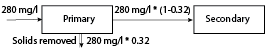
\includegraphics[scale=0.8]{Problem}
\end{center}

Influent BOD concentration to the AS basin: $280\dfrac{mg}{l}*(1-0.32)= 190.4 \dfrac{mg}{l}$\\

$\dfrac{F}{M}= \dfrac{1.5 MGD * 190.4\dfrac{mg}{l}*8.34}{7000*0.79}= \boxed{0.43\dfrac{F}{M}}$
\\

\item Given that an activated sludge plant with an influent flow of 1.2 MGD is operated at an MCRT of 6 days and the parameters below, calculate the WAS flow rate (wasting rate) in gallon per day.
\\

\begin{tabular}{ | m {7 cm} | m {7 cm}| } 
 \hline
Two aeration tanks – 0.5 MG each & Two final clarifiers – 0.25 MG each \\ 
 \hline
 Final effluent $= 20\dfrac{mg}{l}$ & WAS – 7500 ppm\\ 
 \hline
 MLSS –$3600\dfrac{mg}{L}$ & MLSS volatile solids content = 80\%  \\
 \hline
\end{tabular}
\\

MCRT$=\dfrac{lbs MLSS (system)}{\dfrac{lbs}{day}Effluent SS + \dfrac{lbs}{day}WAS SS}  $
\\

\noindent lbs MLSS (system)$=(2*0.5 + 2*0.25)MG * 3600\dfrac{mg}{L} * 8.34 = 45036lbs$
\\

\noindent $\dfrac{lbs}{day} Effluent SS= 1.2 MG * 20\dfrac{mg}{L} * 8.34 = 200.2lbs$
\\

\noindent MCRT: $6 days=\dfrac{45036}{200.2 \dfrac{lbs}{day}+ \dfrac{lbs}{day}WAS SS}  $
\\

\noindent $\dfrac{lbs}{day}WAS SS = \dfrac{45036}{6} - 200.2 = 7306 \dfrac{lbs}{day}$
\\

\noindent $7306 \dfrac{lbs}{day} = WAS Flow (MGD) * 7500 * 8.34 \implies WAS Flow (MGD)=\dfrac{7306}{7500*8.34}=0.116 MGD = \boxed {116,000 \dfrac{gal}{day}}  $







\item Calculate the MCRT of an activated sludge plant given the following information.\\
Plant flow- 4.25 MGD\\
WAS conc-7980 mg/l\\
Waste flow- 0.055 MGD\\
RAS conc.- 7980 mg/l\\
Aeration tank vol-1MG\\  
Clarifier vol- 0.25 MG\\
Final eff TSS conc. - 21.2 mg/l\\
MLSS conc.- 2050 mg/l\\
\vspace{0.3cm}
Solution:\\
\vspace{0.3cm}
$MCRT (days) =  \dfrac{MLSS \enspace in \enspace aeration \enspace tank \enspace (lbs)+MLSS \enspace in \enspace clarifier \enspace (lbs)}{SS \enspace effluent \enspace (lbs/day)+SS \enspace WAS \enspace (lbs/day)}$\\
\vspace{0.3cm} 
$MLSS \enspace in \enspace aeration \enspace tank \enspace (lbs)=1*2050*8.34=17097lbs$\\
\vspace{0.3cm} 
$MLSS \enspace in \enspace clarifier \enspace (lbs)=0.25*2050*8.34=4274.3lbs$\\
\vspace{0.3cm} 
$SS \enspace effluent \enspace (lbs/day)=4.25MGD *21.2mg/l*8.34=751.4lbs/day$\\
\vspace{0.3cm} 
$SS \enspace WAS \enspace (lbs/day)=0.055MGD *7980mg/l*8.34=3660.4lbs/day$\\
\vspace{0.3cm} 
Plugging in the values calculated above: $MCRT (days) =  \dfrac{17097.6+4274.3}{751.4+3660.4}=4.8=\boxed{5days}$\\
\vspace{0.2cm}
\pagebreak

\item Calculate the MCRT given the following.\\
Plant flow - 1.8 MGD\\
MLSS conc -  2800 mg/l\\
WAS flow - 0.04 MGD\\
MLVSS conc. - 2190 mg/l\\
Aerator vol - 0.3 MG\\
Reactor vol. - 0.2 MG\\
RAS conc. - 8150 mg/l\\
Effluent SS conc.-18 mg/l\\
Solution:\\
\vspace{0.2cm}
$MCRT (days) =  \dfrac{MLSS \enspace in \enspace aeration \enspace tank \enspace (lbs)+MLSS \enspace in \enspace clarifier \enspace (lbs)}{SS \enspace effluent \enspace (lbs/day)+SS \enspace WAS \enspace (lbs/day)}$\\
\vspace{0.3cm} 
$MLSS \enspace in \enspace aeration \enspace tank \enspace (lbs)=0.3*2800*8.34=7005.6lbs$\\
\vspace{0.3cm} 
$MLSS \enspace in \enspace clarifier \enspace (lbs)=0.2*2800*8.34=4670.4lbs$\\
\vspace{0.3cm} 
$SS \enspace effluent \enspace (lbs/day)=1.8MGD *18mg/l*8.34=270.2lbs/day$\\
\vspace{0.3cm} 
$SS \enspace WAS \enspace (lbs/day)=0.04MGD *8150mg/l*8.34=2718.8lbs/day$\\
\vspace{0.3cm} 
Plugging in the values calculated above: $MCRT (days) =  \dfrac{7005.6+4670.4}{270.2+2718.8}=3.9=\boxed{4days}$\\
\vspace{0.2cm}
\pagebreak

\item In an aeration tank, the MLSS is 2650 mg/l and recorded 30-minute settling test indicates 221 ml/L.  What is the sludge volume index?\\
\vspace{0.3cm}
Solution:\\
SVI (ml/g)= $\dfrac{Settled \enspace sludge \enspace volume \enspace in \enspace ml/l \enspace after \enspace 30 \enspace min}{MLSS \enspace mg/l}*1000 \dfrac{mg}{g}$\\
\vspace{0.25cm}
SVI=$\dfrac{221ml/l}{2650mg/l}*1000\dfrac{mg}{g}=\boxed{83ml/g}$
\item The desired F/M ratio is .35 lbs BOD/day/lb MLVSS. If 2,100 lbs of BOD enter the aerator daily, how many lbs of MLVSS should be maintained in the aeration tank?\\
Solution:\\
$F:M=\dfrac{(lbs/day) \enspace primary \enspace effluent  \enspace BOD \enspace entering \enspace the  \enspace aeration \enspace tank}{(lbs) \enspace MLVSS \enspace in \enspace the  \enspace aeration \enspace tank}$\\
\vspace{0.3cm}
$\implies 0.35=\dfrac{2100}{x}\implies x = \boxed{130,100lbs \enspace MLVSS}$\\

\item Calculate F/M ratio based on the following data:\\
Secondary influent BOD - 156 mg/l\\
Four (4) aeration basins - 30 ft x 70 ft x 10 ft. deep\\
Influent flow - 0.65 MGD\\
MLSS - 3600 mg/l\\
MLSS average \% volatile - 72\%\\
Solution:\\
\vspace{0.3cm}
$F:M=\dfrac{(lbs/day) \enspace primary \enspace effluent  \enspace BOD \enspace entering \enspace the  \enspace aeration \enspace tank}{(lbs) \enspace MLVSS \enspace in \enspace the  \enspace aeration \enspace tank}$\\
\vspace{0.3cm}
$F:M=\dfrac{156*0.65*8.34}{3600*0.72*4*(30*70*10)ft^3* \dfrac{7.48gal}{ft^3}*\dfrac{MG}{1000000gal}*8.34}=\boxed{0.06}$\\
\pagebreak
\item An activated sludge plant operates well at an F:M ratio of between 0.23 and 0.28.  Calculate the minimum MLSS concentration, given the following:\\
Q = 0.4 MGD\\
Primary influent BOD = 250 mg/l\\
Primary effluent BOD = 128 mg/l\\
Aeration tank vol. = 350,000 gallons\\
Clarifier vol = 250,000 gallons\\
MLSS has 80\% volatile solids\\
Solution:\\
\vspace{0.3cm}
$F:M=\dfrac{(lbs/day) \enspace primary \enspace effluent  \enspace BOD \enspace entering \enspace the  \enspace aeration \enspace tank}{(lbs) \enspace MLVSS \enspace in \enspace the  \enspace aeration \enspace tank}$\\
\vspace{0.3cm}
$\implies F:M \propto \dfrac{1}{MLSS \enspace concentration}$  $\implies$ F:M is inversely proportional to MLSS\\
\vspace{0.3cm}
So to have minimum MLSS conc. F:M needs to be the maximum of the range provided\\
\vspace{0.3cm}
If the MLSS concentration = x:
$ \implies F:M=0.28=\dfrac{0.4*128*8.34}{0.35*x*0.8}\implies x = \boxed{5446 mg/l \enspace MLSS}$
\item 5. Given that an activated sludge plant with an influent flow of 1 MGD is operated at an MCRT of 6 days and the parameters below, calculate the WAS flow rate (wasting rate) in gallon per day.
(10 points)\\
\begin{tabular}{ | m {7 cm} | m {7 cm}| } 
 \hline
Two aeration tanks – 0.45 MG each & Two final clarifiers – 0.2 MG each \\ 
 \hline
 Final effluent $= 16\dfrac{mg}{l}$ & WAS = 6500 ppm\\ 
 \hline
 MLSS =$3000\dfrac{mg}{L}$ & MLSS volatile solids content = 85\%  \\
 \hline
\end{tabular}\vspace{1 cm}
\\
Solution:\\

MCRT$=\dfrac{lbs MLSS (system)}{\dfrac{lbs}{day}Effluent SS + \dfrac{lbs}{day}WAS SS}  $
\\
\vspace{1 cm}
\noindent lbs MLSS (system)$=(2*0.45 + 2*0.2)MG * 3000\dfrac{mg}{L} * 8.34 = 32,526lbs$
\\
\vspace{1 cm}
\noindent $\dfrac{lbs}{day} Effluent SS= 1 MG * 16\dfrac{mg}{L} * 8.34 = 133.4lbs$
\\
\vspace{1 cm}
\noindent MCRT: $6 days=\dfrac{32,526}{133.4 \dfrac{lbs}{day}+ \dfrac{lbs}{day}WAS SS}  $
\\
\vspace{1 cm}
\noindent $\dfrac{lbs}{day}WAS SS = \dfrac{32,526}{6} - 133.4 = 5,288 \dfrac{lbs}{day}$
\\
\vspace{1 cm}
\noindent $5,288 \dfrac{lbs}{day} = WAS Flow (MGD) * 6500 * 8.34$\\
\vspace{1 cm}
$\implies WAS Flow (MGD)=\dfrac{5,288}{6,500*8.34}=0.097546 MGD = \boxed {97,546 \dfrac{gal}{day}}$

\item Operational data is given below for a conventional activated sludge treatment plant:\\

Influent flow: 2.5 mgd\\
Influent BOD: 220 mg/l\\
Influent TSS: 240 mg/l\\
Primary BOD removal efficiency: 30\%\\
Aeration tank volume: 1.8 MG\\
Secondary clarifier volume: 0.8 MG\\
MLSS: 3,600 mg/l\\
MLVSS: 2,800 mg/l\\
RAS SS: 8,500 mg/l\\
RAS VSS: 6,630 mg/l\\
RAS flow: 100\%\\
WAS flow: 35,000 gpd\\
AS Effluent TSS: 25 mg/l\\
AS Effluent BOD: 19 mg/l\\
Settleability results: 60 min= 300 ml/L\\
Settleability results: 30 min= 320 ml/L\\

\begin{enumerate}
\item Calculate the MCRT
\item Calculate the F/M Ratio
\item Calculate the SVI
\end{enumerate}

Solution:\\
\vspace{0.3cm}
\begin{enumerate}
\item $MCRT (days) =  \dfrac{MLSS \enspace in \enspace aeration \enspace tank \enspace (lbs)+MLSS \enspace in \enspace clarifier \enspace (lbs)}{SS \enspace effluent \enspace (lbs/day)+SS \enspace WAS \enspace (lbs/day)}$\\
\vspace{0.3cm} 
$MLSS \enspace in \enspace aeration \enspace tank \enspace (lbs)=1.8*3,600*8.34=54,043lbs$\\
\vspace{0.3cm} 
$MLSS \enspace in \enspace clarifier \enspace (lbs)=0.8*3,600*8.34=24,019lbs$\\
\vspace{0.3cm} 
$SS \enspace effluent \enspace (lbs/day)=2.5MGD *25mg/l*8.34=521lbs/day$\\
\vspace{0.3cm} 
$SS \enspace WAS \enspace (lbs/day)=\dfrac{35,000}{1,000,000}MGD *8,500mg/l*8.34=2,481lbs/day$\\
\vspace{0.3cm} 
$MCRT (days) =  \dfrac{54,043+24,019}{521+2,481}=\boxed{26 \enspace days}$\\
\vspace{0.2cm}
\item $F:M=\dfrac{(lbs/day) \enspace primary \enspace effluent  \enspace BOD \enspace entering \enspace the  \enspace aeration \enspace tank}{(lbs) \enspace MLVSS \enspace in \enspace the  \enspace aeration \enspace tank}$\\
\vspace{0.3cm}
$F:M=\dfrac{220*(1-0.3)*2.5*8.34}{1.8*2,800*8.34}=\boxed{0.08}$\\
\vspace{0.25cm}

\item SVI (ml/g)= $\dfrac{Settled \enspace sludge \enspace volume \enspace in \enspace ml/l \enspace after \enspace 30 \enspace min}{MLSS \enspace mg/l}*1000 \dfrac{mg}{g}$\\
\vspace{0.25cm}
SVI=$\dfrac{320ml/l}{3,600mg/l}*1000\dfrac{mg}{g}=\boxed{89ml/g}$
\end{enumerate}

\item What is the Sludge Volume Index given the following:\\  MLSS = 2800 mg/l; MLVSS 2400 mg/l; Settled Volume after 30 minutes = 250 ml/L\\
\vspace{0.3cm} 
Solution:\\
SVI (ml/g)= $\dfrac{Settled \enspace sludge \enspace volume \enspace in \enspace ml/l \enspace after \enspace 30 \enspace min}{MLSS \enspace mg/l}*1000 \dfrac{mg}{g}$\\
\vspace{0.25cm}
SVI=$\dfrac{250ml/l}{2800mg/l}*1000\dfrac{mg}{g}=\boxed{89ml/g}$

\item Plant Influent Flow:  3.5 MGD\\
Plant Influent BOD:  276 mg/l\\
Primary Treatment BOD Removal:  36\%\\
Desired F/M:  0.3\\
Find lbs of MLVSS that should be maintained in the activated sludge treatment process. (Answer: 17,187 lbs)

\item Given that an activated sludge plant with an influent flow of 1 MGD is operated at an MCRT of 6 days and the parameters below, calculate the WAS flow rate (wasting rate) in gallon per day\\
\begin{tabular}{ | m {7 cm} | m {7 cm}| } 
 \hline
Two aeration tanks – 0.45 MG each & Two final clarifiers – 0.2 MG each \\ 
 \hline
 Final effluent $= 16\dfrac{mg}{l}$ & WAS = 6500 ppm\\ 
 \hline
 MLSS =$3000\dfrac{mg}{L}$ & MLSS volatile solids content = 85\%  \\
 \hline
\end{tabular}\vspace{1 cm}
\\
(Answer: 97,546 gal/day)

\item The aeration tank of a conventional activated sludge plant contains 9300 Ibs of MLSS.  Lab tests show that the MLSS are 79\% volatile solids. The primary effluent contains 2900 Ibs of BOD.  Calculate the F to M ratio for this wastewater treatment plant. (Answer:  0.4)

\item How many lbs of solids are in a 400,000 gallon aeration tank if the suspended solids concentration is 1200 mg/l? (Answer: 4003 lbs)



\item An activated sludge wastewater treatment plant treats an average flow of 3.25 MGD. The aeration tank has a volume of 1.0 MG and a MLSS concentration of 2100 mg/l. The final clarifier has an operating volume of 0.25 MG. Effluent suspended solids concentration averages 21.2 mg/l. The WAS concentration is 8100 mg/l and is wasted at the rate of 0.055 MGD. Calculate the MCRT.

\item What is the F/M ratio on an aeration tank if 1,500 pounds of BOD are added per day and 5000 pounds of volatile solids are under aeration? 

\item In an aeration tank, the MLSS is 2500 mg/l and recorded 30-minute settling test indicates 230 ml.  What is the sludge volume index?



\item An activated sludge aeration tank receives a primary effluent flow of 2.61 MGD with a BOD concentration of 195 mg/l. The mixed liquor volatile suspended solids concentration is 2560 mg/l and the aeration tank volume is 470,000 gallons. What is the current F/M ratio?

\item Calculate the MCRT given the following.
Plant flow- 2.8 MGD\\ 		MLSS conc.- 2800 mg/l\\
WAS flow- 0.07 MGD\\ 		MLVSS conc.- 2190mg/l\\
Aerator volume - 0.38MG\\	RAS SS concentration - 6800 mg/l\\
Clarifier volume - 0.19 MG\\ 	Final effluent TSS - 18 mg/l\\


\item If in a conventional activated sludge treatment plant the aeration tank contains 7000 lbs of MLSS and the final clarifier contains 2500 lbs of MLSS.  If 1300 lbs of solids are wasted each day and 120 lbs of solids leave in the final effluent, Calculate the MCRT.

\item The aeration tank of a conventional activated sludge plant contains 9300 Ibs of MLSS. Lab tests show that the MLSS are 79\% volatile solids. The primary effluent contains twenty-nine hundred pounds (2900 Ibs) of BOD. Calculate the F to M ratio for this wastewater treatment plant.




\item A conventional activated sludge plant receives an average flow of 2.5 MGD. The influent BOD averages 230 and the primary effluent BOD average 160 mg/I. The 0.6 MG aeration tank has a MLSS cone. of 2800 mg/l and a MLVSS cone. of 21 50 mg/l. Calculated the F to M ratio for this plant.




\item A convention activated sludge plant receives an average influent flow of 800,000 gpd. The influent BOD averages 200 mg/l and on the average 32\% of this BOD is removed in the primary sedimentation tank. The mixed liquor tank contains 3250 Ibs of MLSS. These solids contain 77\% volatile matter. Calculate this plant's F to M ratio.

\item In an conventional activated sludge plant calculations show that the aeration tank contains 6500 Ibs of MLSS and the final clarifier contains 2500 Ibs of MLSS. Twelve hundred and fifty pounds (1250 Ibs) of solids is wasted each day and 100 Ibs/day of solids leave in the final effluent. Calculate the MCRT for this plant.


\item A activated sludge plant has a total of 25,000 pounds of solids in the system (i.e. aerator + final clarifier) and has an average effluent flow of 3.75 MGD. The effluent suspended solids concentration averages 22 mg/l. The WAS has a concentration of 7500 mg/l and is being wasted at 0.05 MGD. Calculate the MCRT.


\item An activated sludge wastewater treatment plant discharges an average flow of 3.25· MGD. The mixed liquor tank has a volume of 1.0 MG and a MLSS concentration of 2100 mg/l. The final clarifier has an operating volume of 0.25 MG. Effluent suspended solids concentration averages 21.2 mg/l. The WAS concentration is 8100 j mg/l and is wasted at the rate of 0.055 MGD. Calculate the MCRT.

\item In an conventional activated sludge plant show that the aeration tank contains 6500 Ibs of MLSS and the final clarifier contains 2500 lbs of MLSS. 1250 Ibs of solids is wasted each day and 100 Ibs/day of solids leave in the final effluent. Calculate the MCRT for this plant.  Answer:  7 days

\item An activated sludge plant has a total of 25,000 pounds of solids in the system (aerator + final Clarifier) and has an average effluent flow of 3.75 MGD. The effluent suspended solids concentration averages 22 mg/l. The WAS has a concentration 'of 7500 .mg/l and is being wasted at 0.05 MGD. Calculate the MCRT.  Answer:  7 days

\item An activated sludge wastewater treatment plant discharges an average flow of 3.25 MGD. The mixed liquor tank has a volume of 1.0 MG and a MLSS concentration of 2100 mg/l. The final clarifier has an operating volume of 0.25 MG. Effluent suspended solids concentration averages 21.2 mg/l and the WAS concentration is 8100 mg/l and is wasted at the rate of 0.055 MGD.  Calculate the MCRT.  Answer: 5.1 days

\item A conventional activated sludge plant receives an average flow of 2.5 MGD. The influent BOD averages 230 and the primary effluent BOD averages 160mg/l The 0.6 MG aeration tank has a MLSS conc. of 2800 mg/l and a MLVSS conc. of 2150mg/l. Calculate  the F to M ratio for this plant.  Answer:  0.31

\item A conventional activated sludge plant receives an influent flow of 800,000 gpd. The influent BOD averages 200 mg/l and on the average 32\% of this BOD is removed in the primary sedimentation tank. The mixed liquor tank contains 3250 Ibs of MLSS. These solids contain 77\% volatile matter. Calculate this plant's F to M ratio.  Answer:  0.36

\item Calculate the MCRT given the following.
Plant flow- 1.8 MGD\\ 		MLSS conc.- 2800 mg/l\\
WAS flow- 0.04 MGD \\		MLVSS conc.- 2190mg/l\\
Aerator vol- 0.3MG\\	RAS conc.- 8150 mg/l\\
Clarifier vol- 0.lMG\\ 		Final eff TSS- 26 mg/l\\
Answer: 3 days

\item Calculate the F to M ratio given the following Information.
Plant flow- 3.7 MGD\\		Primary eff TSS- 120mg/l\\
Aerator Vol - 0.85 MG\\ 	MLSS conc.- 3200 mg/l\\
Clarifier Vol - 0.25 MG \\	MLVSS conc.- 2550 mg/l\\
Primary effluent BOD-120 mg/l\\
Answer:  0.2\\

\item Calculate the F to M ratio given the following.
Plant flow- 0.8 MGD
Aerator vol- 200,000 gal.
Clarifier Volume-175,000 gal
Primary eff BOD- 120 mg/l
MLVSS cone. -1950 mg/l\\
Answer:  0.25\\
\vspace{0.3cm}
$F:M=\dfrac{(lbs/day) \enspace primary \enspace effluent  \enspace BOD \enspace entering \enspace the  \enspace aeration \enspace tank}{(lbs) \enspace MLVSS \enspace in \enspace the  \enspace aeration \enspace tank}$\\
\vspace{0.3cm}
$F:M=\dfrac{120*0.8*8.34}{1950*0.2*8.34}=\boxed{0.25}$\\
\item Calculate the MCRT of an activated sludge plant given the following information.
Plant flow- 4.25 MGD\\
WAS conc-7980 mg/l\\
Waste flow- 0.055 MGD\\
RAS conc.- 7980 mg/l\\
Aeration tank vol-1MG\\  
Clarifier vol- 0.25 MG\\
Final eff TSS conc. - 21.2 mg/l\\
MLSS conc.- 2050 mg/l\\
$MCRT (days) =  \dfrac{MLSS \enspace in \enspace aeration \enspace tank \enspace (lbs)+MLSS \enspace in \enspace clarifier \enspace (lbs)}{SS \enspace effluent \enspace (lbs/day)+SS \enspace WAS \enspace (lbs/day)}$\\
\vspace{0.3cm} 
$MLSS \enspace in \enspace aeration \enspace tank \enspace (lbs)=1*2050*8.34=17097lbs$\\
\vspace{0.3cm} 
$MLSS \enspace in \enspace clarifier \enspace (lbs)=0.25*2050*8.34=4274.3lbs$\\
\vspace{0.3cm} 
$SS \enspace effluent \enspace (lbs/day)=4.25MGD *21.2mg/l*8.34=751.4lbs/day$\\
\vspace{0.3cm} 
$SS \enspace WAS \enspace (lbs/day)=0.055MGD *7980mg/l*8.34=3660.4lbs/day$\\
\vspace{0.3cm} 
Plugging in the values calculated above: $MCRT (days) =  \dfrac{17097.6+4274.3}{751.4+3660.4}=4.8=\boxed{5days}$\\
\vspace{0.2cm}


\item Calculate the MCRT given the following.\\
Plant flow - 1.8 MGD\\
MLSS conc -  2800 mg/l\\
WAS flow - 0.04 MGD\\
MLVSS conc. - 2190 mg/l\\
Aerator vol - 0.3 MG\\
Reactor vol. - 0.2 MG\\
RAS conc. - 8150 mg/l\\
Effluent SS conc.-18 mg/l\\
Solution:\\
\vspace{0.2cm}
$MCRT (days) =  \dfrac{MLSS \enspace in \enspace aeration \enspace tank \enspace (lbs)+MLSS \enspace in \enspace clarifier \enspace (lbs)}{SS \enspace effluent \enspace (lbs/day)+SS \enspace WAS \enspace (lbs/day)}$\\
\vspace{0.3cm} 
$MLSS \enspace in \enspace aeration \enspace tank \enspace (lbs)=0.3*2800*8.34=7005.6lbs$\\
\vspace{0.3cm} 
$MLSS \enspace in \enspace clarifier \enspace (lbs)=0.2*2800*8.34=4670.4lbs$\\
\vspace{0.3cm} 
$SS \enspace effluent \enspace (lbs/day)=1.8MGD *18mg/l*8.34=270.2lbs/day$\\
\vspace{0.3cm} 
$SS \enspace WAS \enspace (lbs/day)=0.04MGD *8150mg/l*8.34=2718.8lbs/day$\\
\vspace{0.3cm} 
Plugging in the values calculated above: $MCRT (days) =  \dfrac{7005.6+4670.4}{270.2+2718.8}=3.9=\boxed{4days}$\\
\vspace{0.2cm}

\item The desired F/M ratio is .35 lbs BOD/day/lb MLVSS. If 2,100 lbs of BOD enter the aerator daily, how many lbs of MLVSS should be maintained in the aeration tank?\\
Solution:\\
$F:M=\dfrac{(lbs/day) \enspace primary \enspace effluent  \enspace BOD \enspace entering \enspace the  \enspace aeration \enspace tank}{(lbs) \enspace MLVSS \enspace in \enspace the  \enspace aeration \enspace tank}$\\
\vspace{0.3cm}
$\implies 0.35=\dfrac{2100}{x}\implies x = \boxed{6000lbs \enspace MLVSS}$\\

\item Calculate F/M ratio based on the following data:\\
Secondary influent BOD - 156 mg/l\\
Four (4) aeration basins - 30 ft x 70 ft x 10 ft. deep\\
Influent flow - 0.65 MGD\\
MLSS - 3600 mg/l\\
MLSS average \% volatile - 72\%\\
Solution:\\
\vspace{0.3cm}
$F:M=\dfrac{(lbs/day) \enspace primary \enspace effluent  \enspace BOD \enspace entering \enspace the  \enspace aeration \enspace tank}{(lbs) \enspace MLVSS \enspace in \enspace the  \enspace aeration \enspace tank}$\\
\vspace{0.3cm}
$F:M=\dfrac{156*0.65*8.34}{3600*0.72*4*(30*70*10)ft^3* \dfrac{7.48gal}{ft^3}*\dfrac{MG}{1000000gal}*8.34}=\boxed{0.06}$\\
\vspace{0.3cm}
\item An activated sludge plant operates well at an F:M ratio of between 0.23 and 0.28.  Calculate the minimum MLSS concentration, given the following:
Q = 0.4 MGD
Primary influent BOD = 250 mg/l
Primary effluent BOD = 128 mg/l
Aeration tank vol. = 350,000 gallons
Clarifier vol = 250,000 gallons
MLSS has 80\% volatile solids
Solution:\\
\vspace{0.3cm}
$F:M=\dfrac{(lbs/day) \enspace primary \enspace effluent  \enspace BOD \enspace entering \enspace the  \enspace aeration \enspace tank}{(lbs) \enspace MLVSS \enspace in \enspace the  \enspace aeration \enspace tank}$\\
\vspace{0.3cm}
$\implies F:M \propto \dfrac{1}{MLSS \enspace concentration}$\\
\vspace{0.3cm}
So to have minimum MLSS conc. F:M needs to be the maximum of the range provided\\
\vspace{0.3cm}
If the MLSS concentration = x:
$ \implies F:M=0.28=\dfrac{0.4*128*8.34}{0.35*x*0.8}\implies x = \boxed{5446 mg/l \enspace MLSS}$







\item If the target MCRT for an activated sludge plant with the following parameters is 8 days, what is the required wasting rate (in gallons per day)? (8 points)

Aeration Tank Volume = 1.5 MG\\
Clarifier Volume = 1.2 MG\\
MLSS Concentration = 2500 mg/l\\
MLSS Volatile Solids = 79\%\\
WAS SS = 5100 mg/l\\
Secondary Effluent SS = 12 mg/l\\
Plant flow = 15 MGD\\
$ MCRT = \dfrac{(Total \enspace MLSS \enspace lbs \enspace in \enspace the \enspace aeration \enspace system (aeration \enspace tank\enspace+\enspace clarifier))}{(Total \enspace amount \enspace in \enspace \dfrac{lbs}{day} \enspace of \enspace  SS \enspace leaving \enspace the  \enspace system (effluent+WAS))}$\\
$MCRT =\dfrac{(MLSS\textsubscript{aeration tank} (lbs)\enspace + \enspace MLSS \textsubscript{clarifier} \enspace (lbs))}{(SS \textsubscript{effluent} (lbs/day)+SS \textsubscript{WAS} (lbs/day))}$\\

$\implies 8 days=\dfrac{(1.5 + 1.2)MG * 8.34 * 2500 \dfrac{mg}{l}}{(15 MGD*12\dfrac{mg}{l} *8.34) (lbs/day \enspace SS \textsubscript{effluent}+(xMGD \enspace WAS * 5100\dfrac{mg}{l}*8.34)(lbs/day \enspace SS \textsubscript{WAS})}$

$(15 *12*8.34 (lbs/day)SS \textsubscript{effluent}+xMGD\enspace WAS * 5100*8.34)(lbs/day)SS \textsubscript{WAS}=\dfrac{(1.5 + 1.2)MG * 8.34 * 2500}{8}$

$xMGD\enspace WAS * 5100*8.34(lbs/day)SS \textsubscript{WAS}=\dfrac{(1.5 + 1.2)MG * 8.34 * 2500}{8}-(15 *12*8.34 (lbs/day)SS \textsubscript{effluent}$\\
$42,534x=5535.7\implies x =\dfrac{5535.7}{42,534}=0.1301 MGD = \boxed{130,100\dfrac{gal}{day}}$\\
\vspace {8mm}

\item Given the following:
Plant Influent Flow:  3.5 MGD\\
Plant Influent BOD:  276 mg/l\\
Primary Treatment BOD Removal:  36\%\\
Desired F/M:  0.3\\
Find lbs of MLVSS that should be maintained in the activated sludge treatment process. (7 points)
$F:M = \dfrac{lbs \enspace Influent \enspace BOD}{lbs \enspace MLVSS}\implies 0.3 = \dfrac{276*(1-0.36)*3.5*8.34}{lbs MLVSS} \implies lbs \enspace MLVSS=\boxed{17,187lbs}$

5. Given that an activated sludge plant with an influent flow of 1 MGD is operated at an MCRT of 6 days and the parameters below, calculate the WAS flow rate (wasting rate) in gallon per day.
(10 points)\\
\begin{tabular}{ | m {7 cm} | m {7 cm}| } 
 \hline
Two aeration tanks – 0.45 MG each & Two final clarifiers – 0.2 MG each \\ 
 \hline
 Final effluent $= 16\dfrac{mg}{l}$ & WAS = 6500 ppm\\ 
 \hline
 MLSS =$3000\dfrac{mg}{L}$ & MLSS volatile solids content = 85\%  \\
 \hline
\end{tabular}\vspace{1 cm}
\\
Solution:\\

MCRT$=\dfrac{lbs MLSS (system)}{\dfrac{lbs}{day}Effluent SS + \dfrac{lbs}{day}WAS SS}  $
\\
\vspace{1 cm}
\noindent lbs MLSS (system)$=(2*0.45 + 2*0.2)MG * 3000\dfrac{mg}{L} * 8.34 = 32,526lbs$
\\
\vspace{1 cm}
\noindent $\dfrac{lbs}{day} Effluent SS= 1 MG * 16\dfrac{mg}{L} * 8.34 = 133.4lbs$
\\
\vspace{1 cm}
\noindent MCRT: $6 days=\dfrac{32,526}{133.4 \dfrac{lbs}{day}+ \dfrac{lbs}{day}WAS SS}  $
\\
\vspace{1 cm}
\noindent $\dfrac{lbs}{day}WAS SS = \dfrac{32,526}{6} - 133.4 = 5,288 \dfrac{lbs}{day}$
\\
\vspace{1 cm}
\noindent $5,288 \dfrac{lbs}{day} = WAS Flow (MGD) * 6500 * 8.34$\\
\vspace{1 cm}
$\implies WAS Flow (MGD)=\dfrac{5,288}{6,500*8.34}=0.097546 MGD = \boxed {97,546 \dfrac{gal}{day}}$

\item The desired F/M ratio is 0.35. If 2,100 lbs of BOD enter the aerator daily and the volume of the mixed liquor in the aeration tank is 375,000 gallons , what should be the target MLVSS concentration?\\

Solution:\\
$F:M=\frac{(lbs/day) \enspace primary \enspace effluent  \enspace BOD \enspace entering \enspace the  \enspace aeration \enspace tank}{(lbs) \enspace MLVSS \enspace in \enspace the  \enspace aeration \enspace tank}$\\
\vspace{0.3cm}
$\implies 0.35=\frac{2100}{x}\implies x = \boxed{6000lbs \enspace MLVSS}$\\

\vspace{0.3cm}
$\implies 6,000 lbs \enspace MLVSS=8.34 * \frac{375,000}{1,000,000}MG*x\frac{mg \enspace MLVSS}{L}$\\
$\implies x\frac{mg \enspace MLVSS}{L} = \frac{6000}{8.34*0.375}=\boxed{1,900\frac{mg \enspace MLVSS}{L}}$






























\end{enumerate}


\section*{Solids Treatment Math Problems}
\begin{enumerate}
\item Calculate the volatile solids reduction in an anaerobic digester given the following information: Raw sludge feed to digester: 73.7 \% VS and digested sludge: 57.2 \%VS\\

*a. 52.3\% \\
b. 64\%\\
c. 16.5\% \\
d. 42\% \\
\vspace{0.25cm}
Solution:\\
\vspace{0.25cm}  
The VS reduction of the digester is provided by the Van Kleeck equation \\ 
\vspace{0.25cm}
$Digester \enspace VS \enspace reduction (\%)=\dfrac{VS_{in}-VS_{out}}{VS_{in}-VS_{in}*VS_{out}}*100$\\
\vspace{0.25cm}
$Digester \enspace VS \enspace reduction (\%)=\dfrac{0.737-0.572}{0.737-0.737*0.572}*100=\boxed{ 52.3\%}$\\





\item 42,000 gallons of 6\% sludge containing 67\% volatile matter is pumped to the digester.  The digester reduces the volatile matter by 52\%.  What volume of sludge in gallons containing 5\% solids remains after digestion? [Ans:  32,841 gal]

\item An anaerobic digester is 37’ in diameter and 27’ deep with a 5,000 gallon daily sludge flow. The sludge is 6\% solids and 66\% volatile solids.  What is the volatile solids loading in pounds per cubic foot per day? [0.057 lbs VS/ft3-day]

\item An Imhoff cone result is 5.5 ml/l.  Approximately how many gallons of primary sludge will need to be pumped if the flow is 0.7 MGD? [3,850 gallons]

\item A sludge digester equipped with a floating cover is 31 ft. inside diameter.  The corbels are 16 feet above the floor and the top of the wall is 20 feet above the floor.  The digester currently has a sludge depth of 16.5 ft. How many gallons of sludge are needed to displace the cover 1 foot? [5,643 galllons]

\item 10,000 gallons/day of sludge is pumped to an anaerobic digester/day at 4\% solids (70\% VS).  If 50\% of the VS is destroyed, how many lbs of VS is destroyed per day?\\
Solution:\\
$\frac{10,000 \enspace Gal}{day}*\frac{8.34 \enspace lbs \enspace sludge}{Gal} \frac{0.04*0.7 \enspace lbs \enspace VS \enspace feed}{lb \enspace sludge}*\frac{0.5 \enspace lbs \enspace VS \enspace destroyed}{lbs \enspace VS \enspace feed}=\boxed{\frac{1,168lbs \enspace VS \enspace destroyed}{day} } $


\item Two sludges are blended together as follows: 15,000 gal. primary sludge at 4.1\% solids. 28,000 gal. secondary sludge at 1.3\% solids. What is the combined solids concentration? [Ans. 2.28\%] If the primary sludge is 68\% VS and the secondary sludge is 63\% VS, how many pounds of VS are in the combined sludge? [Ans. 5400.3 lbs VS]


\item 12,000 gallons of 1.8\% sludge is pumped to a thickener, and is thickened to 3800 gallons of 4.9\% solids. The supernatant is returned back to the head of the STP for treatment.  What is the volume in gallons and solids concentration in ppm of the supernatant?[Ans. 24,980 gallons]


\item How many pounds of solids are pumped to a digester each day if the digester receives 10,000 gpd of sludge at 5\% solids concentration?\\


 

Solution:\\

{
$
	\dfrac{lbs \enspace TS}{day}
	=
	\dfrac{10,000 gal \enspace sludge}{day}
	*
	\dfrac{(8.34*0.05 lbs TS )}{gal \enspace sludge}
	=4,170
	\dfrac{lbs \enspace TS}{day}
$
}\\


\item Calculate the \% VS reduction in a digester given the volatile solids content of the influent sludge to the digester is 70\% and the volatile solids content of the sludge leaving the digester is 52.5\%\\
Solution:  $Digester \enspace VS \enspace reduction (\%)=\dfrac{0.7-0.525}{0.7-0.7*0.525}*100=\boxed{ 53\%}$\\

\item If an anaerobic digester receives sludge with VS of 80\% and discharges digested sludge with a 60\% VS. Its VS reduction is:\\
a. 20\% \\
b. 25\% \\
c. 63\% \\
d. 89\% \\
\vspace{0.25cm}
Solution:\\
\vspace{0.25cm}
$Digester \enspace VS \enspace reduction (\%)=\dfrac{0.8-0.6}{0.8-0.8*0.6}*100=\boxed{ 63\%}$\\

\vspace{0.25cm}
\item Calculate the VS loading to the digester in lbs/day if 10,000 gallons of sludge containing 5\% TS with and average VS content of 78\%\\
Solution:\\
Digester VS loading (lbs/day)\\$=\dfrac{10,000 \enspace gallons \enspace sludge}{day}*\dfrac{8.34lbs \enspace sludge}{gal}*\dfrac{0.05*0.78lbs VS}{lb \enspace sludge}=\boxed{3,253lbs \enspace sludge \enspace per \enspace day}$

\item Primary sludge containing five percent (5\%) solids is pumped to a digester continuously at a rate of 25 gpm. How many pounds of volatile solids are added to the digester each day if the volatile solids content is 73\% of the total solids?\\
a. 1,310 lbs/day \\
b. 1,800 lbs/day \\
c. 9,830 lbs/day \\
d. 10,960 lbs/day \\
e. 15,010 lbs/day \\
\vspace{0.25cm}
Solution:\\
\vspace{0.25cm}
Digester VS loading (lbs/day)\\$=\dfrac{25*1,440 \enspace gallons \enspace sludge}{day}*\dfrac{8.34lbs \enspace sludge}{gal}*\dfrac{0.05*0.73lbs VS}{lb \enspace sludge}=\boxed{10,960 \enspace lbs \enspace sludge \enspace per \enspace day}$\\
\vspace{0.25cm}






\item An anaerobic digester is 37’ in diameter and 27’ deep with a 5,000 gallon daily sludge flow. The sludge is 6\% solids and 66\% volatile solids.  What is the volatile solids loading in pounds per cubic foot per day?
	
	
Solution:\\
{
$
	Digester \enspace volatile \enspace solids 			\enspace loading \enspace rate = 					\dfrac
	{
	Digester \enspace Loading 
		\dfrac
		{
		lbs \enspace VS
		}
		{
		day
		}
	}
	{
	Digester \enspace volume (V)ft^3
	}
$
}\\
\begin{center}
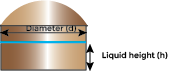
\includegraphics[scale=1]{DigesterWOCDimensions_1}
\end{center}

{
$=\dfrac
	{
		5000
		\dfrac
			{gal \enspace sludge}
			{day}
		*(8.34*0.06*0.66) 
		\dfrac
			{lbs VS}
			{gal \enspace  sludge}
	}
	{
		(\dfrac
			{\pi}
			{4}*37^2*27)ft^3
	}
=\boxed
	{
		0.057 \dfrac
			{lbs \enspace VS}
			{day-ft^3}
	}
$}


\item How much gas is produced in the above digester in $ft^3$/day if the digested sludge contains 2.5\% total solids of which 59\% is volatile solids and the gas production rate is 14 $ft^3$/lb VS destroyed?\\
Solution:\\

{
$
Digester \enspace VS \enspace reduction (\%)=
	\dfrac
	{0.70 - .59}
	{0.70 - 0.70 *0.59}
	*100=38.3\%
$
}\\
\vspace{6mm}

{
$
	\dfrac
	{
	lbs \enspace VS \enspace reduction
	}
	{
	day
	}
	=
	\dfrac
	{
	3153 lbs \enspace VS \enspace feed
		*  0.383 \enspace VS \enspace reduction
	}
	{
	day
	}
 	=1,208
	\dfrac
	{
	lbs \enspace VS \enspace reduction
	}
	{
	day 
	}
$
}\\
\vspace{6mm}

{
$
	\dfrac 
	{
	ft^3 gas \enspace produced
	}
	{
	day
	}
	=
	1208 \dfrac
			{
			lbs \enspace VS \enspace reduced
			}
			{
			day
			}
			*
		\dfrac
		{
		14 ft^3 \enspace gas \enspace produced
		}
		{
		lb \enspace VS \enspace reduced
		}
		=16,912 \dfrac
				{
				ft^3 \enspace digester \enspace 					gas \enspace produced
				}
				{
				day
				}
$
} 
\item The sludge feed to a digester is 80,000 gal/day. The sludge contains 4.5\% total solids with 75\% volatile solids. If 50\% of VS are reduced in the digester: 



\begin{enumerate}
\item Find lbs VS destroyed per 1000 gal of digester capacity per day if the digester radius is 55 ft with an operating sludge level of 25 ft.(5 points)

\vspace{1cm}
Solution:\\
Digester Volume: 
$
{
		(\pi*55^2*25)ft^3 *7.48 \dfrac{gal}{ft^3}
	}=1,776,220 gallons=1,776.2 \enspace(1000 \enspace gallons)
$
\\
\vspace{3mm}
$
	\dfrac
	{
	lbs \enspace VS \enspace reduction
	}
	{
	day
	}
	=
	\dfrac
	{
	80,000 gal * 8.34 \dfrac{lbs}{gal}*(0.045*0.75) \dfrac{lbs VS}{lb}*0.5\dfrac{lbs \enspace VS \enspace  reduction}{lb \enspace VS}
	}
	{
	day
	}$\\
\vspace{0.25cm}
$
 	=11,259
	\dfrac
	{
	lbs \enspace VS \enspace reduction
	}
	{
	day 
	}
$
\\
\vspace{3mm}


$
	\dfrac
	{
	lbs \enspace VS \enspace reduction
	}
	{
	1000 \enspace digester \enspace capacity
	}
	=
	\dfrac
	{
	11,259 \dfrac
			{
			lbs \enspace VS \enspace reduction
			}
			{
			day
			}
	}
	{	
	1,776.2 \enspace (1000 \enspace gallons)
	}
 	=\boxed{6.3
	\dfrac
	{
	lbs \enspace VS \enspace reduction
	}
	{
	1000 gallons \enspace digester \enspace volume 
	}}
$
\\

\vspace{1cm}

\item  What is the digester gas production in Btu/day? Assume 14 cu. ft digester gas per lb of VS destroyed and a 650 Btu/cu. ft heating value for the digester gas produced (5 points)
\end{enumerate}
\vspace{1cm}
Solution:\\

$
	\dfrac 
	{
	ft^3 gas \enspace produced
	}
	{
	day
	}
	=
	11,259 \dfrac
			{
			lbs \enspace VS \enspace reduced
			}
			{
			day
			}
			*
		\dfrac
		{
		14 ft^3 \enspace gas \enspace produced
		}
		{
		lb \enspace VS \enspace reduced
		}
		=157,626 \dfrac
				{
				ft^3 \enspace digester \enspace 					gas \enspace produced
				}
				{
				day
				}
$
\\
\vspace{1cm}


$
	\dfrac 
	{
	BTU \enspace produced
	}
	{
	day
	}
	=
	157,626 \dfrac
			{
			ft^3 \enspace gas \enspace produced
			}
			{
			day
			}
			*
		\dfrac
		{
		650 BTU \enspace gas \enspace produced
		}
		{
		ft^3 gas
		}
		=\boxed{102,456,900 \dfrac
				{
				BTU \enspace produced
				}
				{
				day
				}}
$



\item The volatile acids concentration of sludge in an anaerobic digester is 195 mg/l. If the maximum volatile acids:alkalinity ratio is 0.087, what should the alkalinity be in mg/l?\\
Solution:\\
Volatile acid:Alkalinity=0.087=$\dfrac{195}{x}\implies x = \dfrac{195}{0.087} =\boxed{2,241\dfrac{mg}{l}}$
\pagebreak
	
\item 10,000 gallons of sludge is pumped to an anaerobic digester/day at 4\% solids (70\% VS).  50\% of the VS are destroyed, creating 15 $ft^3$ of gas per lbs. of VS destroyed. How much gas is produced each day?\\

{
$
	\dfrac
	{
	lbs \enspace VS \enspace reduction
	}
	{
	day
	}
	=
	\dfrac
	{
	10,000 gal * 8.34 \dfrac{lbs}{gal}*(0.04*0.7) \dfrac{lbs VS}{lb}*\dfrac{0.5 lbs \enspace VS \enspace  reduction}{lb \enspace VS}
	}
	{
	day
	}
 	=1,168
	\dfrac
	{
	lbs \enspace VS \enspace reduction
	}
	{
	day 
	}
$
}\\
\vspace{3mm}

{
$
	\dfrac 
	{
	ft^3 gas \enspace produced
	}
	{
	day
	}
	=
	1,168 \dfrac
			{
			lbs \enspace VS \enspace reduced
			}
			{
			day
			}
			*
		\dfrac
		{
		15 ft^3 \enspace gas \enspace produced
		}
		{
		lb \enspace VS \enspace reduced
		}
		=17,520 \dfrac
				{
				ft^3 \enspace digester \enspace 					gas \enspace produced
				}
				{
				day
				}
$
} 


\item Given a sludge flow of 5,500 gpd with 6.5\% solids containing  72\% VS to a digester with a VS destruction of 48\%   If the digester is digester is 40 ft. diameter with a sludge level of 25 ft, find lbs. VS destroyed per 1000 gal of digester capacity per day.  What is the digester gas production in Btu/day if the \% VS reduction in the digester is 58\% and the digester raw sludge feed is 6000 cu. Ft/day containing 4.5\% total solids with a 64\% VS content?  Assume 13.5 cu. ft digester gas per lb of VS destroyed and a 650 Btu/cu. ft heating value for the digester gas produced\\

{
Digester Volume: 
$
{
		(\dfrac
			{\pi}
			{4}*40^2*25)ft^3 *7.48 \dfrac{gal}{ft^3}
	}=940,086 gallons=940 \enspace(1000 \enspace gallons)
$
}\\
\vspace{3mm}

{
$
	\dfrac
	{
	lbs \enspace VS \enspace reduction
	}
	{
	day
	}
	=
	\dfrac
	{
	5,500 gal * 8.34 \dfrac{lbs}{gal}*(0.065*0.72) \dfrac{lbs VS}{lb}*\dfrac{0.48 lbs \enspace VS \enspace  reduction}{lb \enspace VS}
	}
	{
	day
	}
 	=1,030
	\dfrac
	{
	lbs \enspace VS \enspace reduction
	}
	{
	day 
	}
$
}\\
\vspace{3mm}


{
$
	\dfrac
	{
	lbs \enspace VS \enspace reduction
	}
	{
	1000 \enspace digester \enspace capacity
	}
	=
	\dfrac
	{
	1,030 \dfrac
			{
			lbs \enspace VS \enspace reduction
			}
			{
			day
			}
	}
	{	
	940 \enspace (1000 \enspace gallons)
	}
 	=1.1
	\dfrac
	{
	lbs \enspace VS \enspace reduction
	}
	{
	1000 gallons \enspace digester \enspace volume 
	}
$
}\\
\vspace{3mm}


{
$
	\dfrac 
	{
	ft^3 gas \enspace produced
	}
	{
	day
	}
	=
	1,030 \dfrac
			{
			lbs \enspace VS \enspace reduced
			}
			{
			day
			}
			*
		\dfrac
		{
		13.5 ft^3 \enspace gas \enspace produced
		}
		{
		lb \enspace VS \enspace reduced
		}
		=13,905 \dfrac
				{
				ft^3 \enspace digester \enspace 					gas \enspace produced
				}
				{
				day
				}
$
}\\
\vspace{3mm}



{
$
	\dfrac 
	{
	BTU \enspace produced
	}
	{
	day
	}
	=
	13,905 \dfrac
			{
			ft^3 \enspace gas \enspace produced
			}
			{
			day
			}
			*
		\dfrac
		{
		650 BTU \enspace gas \enspace produced
		}
		{
		ft^3 gas
		}
		=9,038,250 \dfrac
				{
				BTU \enspace produced
				}
				{
				day
				}
$
}

\item Two sludges are blended together as follows: 60,000 gal per day. primary sludge at 4.5\% solids and 28,000 gal secondary sludge at 5\% solids. 
\begin{enumerate}
\item What is the combined solids concentration?  (3 points)\\

$\dfrac{60,000*4.5+28,000*5}{88,000}=\boxed{4.66\%}$\\
\vspace{2cm}
\item How many lbs of solids (per day) are in the combined sludge (3 points)\\

$88,000 gal*8.34*0.0466 = \boxed{34,200 lbs}$\\
\vspace{2cm}


\item If the primary sludge is 68\% VS and the secondary sludge is 83\% VS, how many pounds of VS are in the combined sludge? (3 points)\\
$60,000 gal *\dfrac{8.34*0.045*0.68lbs \enspace VS}{gal}+28,000 gal *\dfrac{8.34*0.05*0.83lbs \enspace VS}{gal}=\boxed{25,003 lbs \enspace VS}$
\vspace{2cm}

\item What is the digester feed VS\%?  (3 points)\\
$\dfrac{25,003 lbs \enspace VS}{34,200 lbs TS}=\boxed{73.1\%}$

\vspace{2cm}



\item If the digester is 120’ diameter with a liquid height of 20’, what is the VS loading in lbs VS/ft3-day (3 points)\\

$\dfrac{25,003 lbs \enspace VS}{0.785*120^2*20}=\boxed{\dfrac{0.11 lbs \enspace VS}{day-ft^3}}$\\
\vspace{2cm}





\item If the digested sludge has 52\% VS, calculate the digester VS reduction percent (3 points)\\

$
Digester \enspace VS \enspace reduction (\%)=
	\dfrac
	{0.731 - .52}
	{0.731 - 0.731 *0.52}
	*100=\boxed{60.1\%}
$\\
\vspace{2cm}

\item What is the gas production (ft$^3$/day) if the digester produces 14 ft$^3$ gas/lb VS destroyed (3 points)\\
25,003*0.601$\dfrac{lbs\enspace VS destroyed}{}*\dfrac{14ft^3 \enspace gas \enspace produced}{lb \enspace VS \enspace destroyed}=\boxed{210,375ft^3 gas}$
\\
\vspace{2cm}

\item How many belt presses are needed to keep up with the digested sludge flow if the belt presses can be operated at a maximum flow of 50 GPM (3 points)\\

88,000$\dfrac{gal \enspace sludge}{day}*\dfrac{day}{1440min}=61 GPM$\\
@50 GPM per press - $\boxed{2 \enspace BFP \enspace required}$
\vspace{2cm}
\item If the digested sludge feed to the belt filter presses is 2.6\% and assuming the belt press feed solids capture is 90\%.  How many lbs of solids (dry) are produced by the BFP (4 points)\\
$88,000\dfrac{gal}{day}*8.34*0.026\dfrac{lbs \enspace solids \enspace feed}{day}*0.9\dfrac{lbs \enspace solids \enspace captured}{lbs \enspace solids \enspace feed}=\boxed{17,174 lbs \enspace solids \enspace per \enspace day}$
\vspace{2cm}

\item If the BFP produces a 20\% cake, how many wet tons cake produced per day (4 points)\\
$\dfrac{17,174 lbs \enspace solids \enspace produced}{day}*\dfrac{100 lbs \enspace cake}{20 lbs \enspace solids \enspace produced}*\dfrac{tons}{2,000 lbs}=\boxed{\dfrac{42.9tons}{day}}$
\vspace{2cm}

\item If the cake density is 68 lbs/cu. ft, how much time will it take to fill a 30 cu. yd bin (3 points)\\
(Ans. 15.4 hours)
$\dfrac{(42.9*2000)lbs \enspace cake}{day}*\dfrac{day}{1440 min}=\dfrac{59.583}{lbs \enspace cake}{min}$\\
$\dfrac{59.583}{lbs \enspace cake}{min}*\dfrac{ft^3}{68 lbs \enspace cake}=\dfrac{0.876ft^3}{min}$\\
$30yd^3*\dfrac{27ft^3}{yd^3}*\dfrac{min}{0.876ft^3}*\dfrac{hrs}{60 min}=\boxed{15.4hrs}$
\vspace{2cm}
\item What will be the cost of hauling dewatered cake per day @ \$65 per ton cake (2 points)\\
42.9$\dfrac{tons}{day}*\dfrac{\$65}{ton}=\boxed{\dfrac{\$2,789}{day}}$ 
\end{enumerate}

\item Calculate the VS loading to the digester in lbs/day if 25,000 gallons of sludge containing 4.5\% TS with and average VS content of 76\% is fed to the digester 


\item Calculate the organic loading rate to two 320,000 gallon anaerobic digesters given:
Primary sludge feed rate of 25,000 gallons with 6.2\% TS containing 73\% solids and SG of 1.03.
Secondary sludge feed rate of 30,500 gallons with 3.8\% TS containing 77\% solids (7 points)
(Answer: 0.2lbs VS/day-ft3 ) 



\item Calculate the organic loading rate to two 320,000 gallon anaerobic digesters given:\\
Primary sludge feed rate of 25,000 gallons with 3.8\% TS containing 73\% solids and SG of 1.03.\\
Secondary sludge feed rate of 30,500 gallons with 3.8\% TS containing 77\% solids 
\\
(Answer: 0.2 $\dfrac{lbs \enspace VS}{day-ft^3}$)\\
\vspace{1cm}



\item 325 GPM of WAS with 7,000 mg/l TSS is thickened in a DAFT.  Assuming an air:solids ratio of 0.05 lb of air for each lb of feed solids, The SCFM (standard cubic feed per minute) air required to thicken the WAS given 1 SCFM = 0.075 lb is:\\
(Answer:  $12.6 \enspace SCFM$)\\
Solution:\\

Correct Answer:\\
$0.05=\dfrac{lb \enspace air}{lb \enspace solids}=\dfrac{\dfrac{0.075 \enspace lbs  \enspace air}{SCF}*x \enspace SCFM}{(\dfrac{325}{1,000,000}MG \enspace per \enspace min*7000*8.34) \enspace lbs  \enspace solids}$\\
\vspace{0.25cm}

$\implies x \enspace SCFM=\dfrac{0.05*325*7000*8.34}{0.075*1,000,000}=\boxed{12.6 \enspace SCFM} - Correct \enspace answer$\\
\vspace{0.25cm}
Incorrect Answer \#1:\\
12,600SCFM

\vspace{0.25cm}
Incorrect Answer \#2:\\
0.126SCFM


\vspace{0.25cm}
Incorrect Answer \#3:\\
1.26SCFM

\vspace{1cm}



\item 30,000 gpd of 4.5\% sludge is dewatered in a centrifuge yielding 24.5 $yd^3/day$ of 25\% cake with a density of 65 lb per $ft^3$.  Calculate the percentage solids recovery.\\
(Answer: 95.5\%)\\
\vspace{1cm}

\item Estimate the amount of heat value of the gas produced from an anaerobic digester in $\dfrac{BTU}{day}$ given the following: \\  
\renewcommand{\arraystretch}{0.6}
\begin{tabular}{ | m {7 cm} | m {4 cm}| } 
 \hline
Raw sludge pumping schedule & 12 min/hr \\ 
 \hline
Sludge pumping rate & 68 GPM\\ 
 \hline
 Raw sludge \%TS & 5.2\%  \\
 \hline
  Raw sludge \%VS & 72.5\%  \\
 \hline
Gas production & $\dfrac{12 ft^3}{lb \enspace VS \enspace destroyed \enspace - \enspace day}$\\
 \hline
 Percent $CO_2$ & 34\%\\ 
 \hline
 Other gases & 1\%  \\
 \hline
  Pure methane net heat value & 932 $\dfrac{BTU}{ft^3}$\\
 \hline
\end{tabular}\\
\vspace{0.3 cm}
(Answer: 23,146,220 $\dfrac{BTU}{day}$)

\item 12,000 $ft^3$ of anaerobically digested sludge containing 2.8\% TS is dewatered in a centrifuge.  The centrifuge yields 37 $yd^3$ of 26\% of dewatered cake with a density of 73 lb/$ft^3$.  Calculate the solids capture rate.\\


 

Solution:\\
$
	lbs \enspace TS \enspace feed \enspace to \enspace centrifuge
	=
	12,000 ft^3 \enspace sludge
	*
	7.48 
	\dfrac
	{
	gal
	}
	{
	ft^3
	}
	*
	\dfrac
	{
	(8.34*0.028 lbs \enspace TS )
	}
	{gal \enspace sludge
	}
	=20,960 {lbs \enspace TS}
$

$
	lbs \enspace TS \enspace feed \enspace from \enspace centrifuge
	=
	37 yd^3 \enspace sludge
	*
	27 
	\dfrac
	{
	ft^3
	}
	{
	yd^3
	}
	*
	\dfrac
	{
	(73 lbs *0.26 \enspace TS )
	}
	{ft^3 \enspace sludge
	}
	=18,961 {lbs \enspace TS}
$

$
	solids \enspace capture \enspace rate
	=
	\dfrac
	{
	18,961 lbs \enspace solids \enspace produced 		\enspace by \enspace centrifuge
	}
	{
	20,960 lbs \enspace solids \enspace fed 			\enspace from \enspace digester
	}
	*
	100 
	=\boxed
	{
	90.4\% solids \enspace capture
	}
$


\item At a 60 GPM of 2.8\% feed a belt press which has a 90\% solids capture rate produces a 20\% cake at 68 lbs/$ft^3$.  How long would it take to fill a 3 $yd^3$ bin  
	
	
Solution:\\
Approach:
\begin{itemize}
\item First calculate the amount of cake solids produced in terms of weight per time.
\item From the weight of the cake produced calculate the volume time, and finally
\item using the calculated value of the volume of the cake produced per time, calculate the time required to fill the bin\\
\end{itemize}

$\dfrac{cake \enspace TS \enspace produced - lbs}{min}= \dfrac {60 gallons \enspace sludge}{min}*\dfrac {8.34 lbs \enspace sludge \enspace feed}{galllon}*\dfrac{0.028 lbs \enspace TS}{lb \enspace sludge}*0.9$\\
\vspace{3mm}

$=\dfrac{12.61lbs \enspace TS}{min}$\\
\vspace{3mm}

$\dfrac{ft^3 \enspace cake \enspace produced}{min}=\dfrac{12.61lbs \enspace TS}{min}*\dfrac{100 lbs \enspace cake}{20lbs \enspace TS}*\dfrac{ft^3 \enspace cake}{68 lbs \enspace cake} = \dfrac{0.927ft^3 cake}{min}$\\
\vspace{3mm}

$\dfrac{ft^3 \enspace cake \enspace produced}{min}=\dfrac{12.61lbs \enspace TS}{min}*\dfrac{100 lbs \enspace cake}{20lbs \enspace TS}*\dfrac{ft^3 \enspace cake}{68 lbs \enspace cake} = \dfrac{0.927ft^3 cake}{min}$\\
\vspace{3mm}
$Time \enspace required \enspace to \enspace fill \enspace the \enspace bin=\dfrac{min}{0.927ft^3}*{3yd^3}*\dfrac{27ft^3}{yd^3}=\boxed{75min}$\\
\pagebreak
\item Calculate the annual cost savings for an improvement of cake solids from 20\% to 21\% if 400 wet tons (@ 20\% cake) are produced each day and the average cake hauling and disposal cost is \$65 per wet ton.\\
$Total \enspace (dry)\enspace solids \enspace produced \enspace per \enspace day =\dfrac{400 \enspace wet \enspace tons}{day}*\dfrac{20 tons \enspace solids}{100 wet \enspace tons}={80 tons \enspace solids}$\\
\vspace{3mm}
$Tons \enspace wet \enspace cake \enspace@ 21\% \enspace solids =\dfrac{80 \enspace tons \enspace solids}{day}*\dfrac{100 wet \enspace tons}{21 tons \enspace solids}$

\vspace{3mm}
$=\dfrac{380 tons \enspace  wet \enspace solids}{day}$\\
\vspace{3mm}
$Net \enspace savings \enspace (\$/yr) = (400 - 380)\dfrac{wet \enspace tons}{day}*365*\dfrac{days}{yr}*\dfrac{\$65}{wet \enspace ton}=\boxed{\$474,500 \enspace per \enspace year}$


\textbf {NOTE:  General formula for future reference: So if the cake dryness goes up from 20\% to 26\% and currently a utility is spending \$1,000,000 per year for biosolids hauling and disposal, their net savings will be: (26-20)/26*1,000,000 = \$230,769.  Conversely say if the dewatering cake solids drops to 18\%, the net impact will be: (18-20)/18*1,000,000 = \$-111,111 (loss or extra cost).}
\\

\item Two sludges are blended together as follows: 60,000 gal per day. primary sludge at 4.5\% solids and 28,000 gal secondary sludge at 5\% solids. 
\begin{enumerate}
\item What is the combined solids concentration?  (3 points)\\

$\dfrac{60,000*4.5+28,000*5}{88,000}=\boxed{4.66\%}$\\
\vspace{0.25cm}
\item How many lbs of solids (per day) are in the combined sludge (3 points)\\

$88,000 gal*8.34*0.0466 = \boxed{34,200 lbs}$\\
\vspace{0.25cm}


\item If the primary sludge is 68\% VS and the secondary sludge is 83\% VS, how many pounds of VS are in the combined sludge? (3 points)\\
$60,000 gal *\dfrac{8.34*0.045*0.68lbs \enspace VS}{gal}+28,000 gal *\dfrac{8.34*0.05*0.83lbs \enspace VS}{gal}=\boxed{25,003 lbs \enspace VS}$
\vspace{2cm}

\item What is the digester feed VS\%?  (3 points)\\
$\dfrac{25,003 lbs \enspace VS}{34,200 lbs TS}=\boxed{73.1\%}$
\vspace{0.25cm}

\item If the digester is 120’ diameter with a liquid height of 20’, what is the VS loading in lbs VS/ft3-day (3 points)\\

$\dfrac{25,003 lbs \enspace VS}{0.785*120^2*20}=\boxed{\dfrac{0.11 lbs \enspace VS}{day-ft^3}}$\\
\vspace{0.25cm}

\item If the digested sludge has 52\% VS, calculate the digester VS reduction percent (3 points)\\

$
Digester \enspace VS \enspace reduction (\%)=
	\dfrac
	{0.731 - .52}
	{0.731 - 0.731 *0.52}
	*100=\boxed{60.1\%}
$\\
\vspace{0.25cm}

\item What is the gas production (ft$^3$/day) if the digester produces 14 ft$^3$ gas/lb VS destroyed (3 points)\\
25,003*0.601$\dfrac{lbs\enspace VS destroyed}{}*\dfrac{14ft^3 \enspace gas \enspace produced}{lb \enspace VS \enspace destroyed}=\boxed{210,375ft^3 gas}$
\\
\vspace{0.25cm}

\item How many belt presses are needed to keep up with the digested sludge flow if the belt presses can be operated at a maximum flow of 50 GPM (3 points)\\

88,000$\dfrac{gal \enspace sludge}{day}*\dfrac{day}{1440min}=61 GPM$\\
@50 GPM per press - $\boxed{2 \enspace BFP \enspace required}$
\vspace{0.25cm}
\item If the digested sludge feed to the belt filter presses is 2.6\% and assuming the belt press feed solids capture is 90\%.  How many lbs of solids (dry) are produced by the BFP (4 points)\\
$88,000\dfrac{gal}{day}*8.34*0.026\dfrac{lbs \enspace solids \enspace feed}{day}*0.9\dfrac{lbs \enspace solids \enspace captured}{lbs \enspace solids \enspace feed}=\boxed{17,174 lbs \enspace solids \enspace per \enspace day}$
\vspace{0.25cm}

\item If the BFP produces a 20\% cake, how many wet tons cake produced per day (4 points)\\
$\dfrac{17,174 lbs \enspace solids \enspace produced}{day}*\dfrac{100 lbs \enspace cake}{20 lbs \enspace solids \enspace produced}*\dfrac{tons}{2,000 lbs}=\boxed{\dfrac{42.9tons}{day}}$
\vspace{0.25cm}

\item If the cake density is 68 lbs/cu. ft, how much time will it take to fill a 30 cu. yd bin (3 points)\\
(Ans. 15.4 hours)
$\dfrac{(42.9*2000)lbs \enspace cake}{day}*\dfrac{day}{1440 min}=\dfrac{59.583}{lbs \enspace cake}{min}$\\
$\dfrac{59.583}{lbs \enspace cake}{min}*\dfrac{ft^3}{68 lbs \enspace cake}=\dfrac{0.876ft^3}{min}$\\
$30yd^3*\dfrac{27ft^3}{yd^3}*\dfrac{min}{0.876ft^3}*\dfrac{hrs}{60 min}=\boxed{15.4hrs}$
\vspace{0.25cm}
\item What will be the cost of hauling dewatered cake per day @ \$65 per ton cake (2 points)\\
42.9$\dfrac{tons}{day}*\dfrac{\$65}{ton}=\boxed{\dfrac{\$2,789}{day}}$
\end{enumerate}

\item 12,000 $ft^3$ of anaerobically digested sludge containing 2.8\% TS is dewatered in a centrifuge.  The centrifuge yields 37 $yd^3$ of 26\% of dewatered cake with a density of 73 lb/$ft^3$.  Calculate the solids capture rate.\\


 

Solution:\\
{
$
	lbs \enspace TS \enspace feed \enspace to \enspace centrifuge
	=
	12,000 ft^3 \enspace sludge
	*
	7.48 
	\dfrac
	{
	gal
	}
	{
	ft^3
	}
	*
	\dfrac
	{
	(8.34*0.028 lbs \enspace TS )
	}
	{gal \enspace sludge
	}
	=20,976 {lbs \enspace TS}
$
}

{
$
	lbs \enspace TS \enspace feed \enspace from \enspace centrifuge
	=
	37 yd^3 \enspace sludge
	*
	27 
	\dfrac
	{
	ft^3
	}
	{
	yd^3
	}
	*
	\dfrac
	{
	(73 lbs *0.26 \enspace TS )
	}
	{ft^3 \enspace sludge
	}
	=18,961 {lbs \enspace TS}
$
}

{
$
	solids \enspace capture \enspace rate
	=
	\dfrac
	{
	18,961 lbs \enspace solids \enspace produced 		\enspace by \enspace centrifuge
	}
	{
	20,976 lbs \enspace solids \enspace fed 			\enspace from \enspace digester
	}
	*
	100 
	=\boxed
	{
	90.4\% solids \enspace capture
	}
$
}

\item At a 60 GPM of 2.8\% feed a belt press which has a 90\% solids capture rate produces a 20\% cake at 68 lbs/$ft^3$.  How long would it take to fill a 3 $yd^3$ bin  
	
	
Solution:\\
Approach:
\begin{itemize}
\item First calculate the amount of cake solids produced in terms of weight per time.
\item From the weight of the cake produced calculate the volume time, and finally
\item using the calculated value of the volume of the cake produced per time, calculate the time required to fill the bin\\
\end{itemize}

{$\dfrac{cake \enspace TS \enspace produced - lbs}{min}= \dfrac {60 gallons \enspace sludge}{min}*\dfrac {8.34 lbs \enspace sludge \enspace feed}{galllon}*\dfrac{0.028 lbs \enspace TS}{lb \enspace sludge}*0.9$}\\
\vspace{3mm}

{$=\dfrac{12.61lbs \enspace TS}{min}$}\\
\vspace{3mm}

{$\dfrac{ft^3 \enspace cake \enspace produced}{min}=\dfrac{12.61lbs \enspace TS}{min}*\dfrac{100 lbs \enspace cake}{20lbs \enspace TS}*\dfrac{ft^3 \enspace cake}{68 lbs \enspace cake} = \dfrac{0.927ft^3 cake}{min}$}\\
\vspace{3mm}

{$\dfrac{ft^3 \enspace cake \enspace produced}{min}=\dfrac{12.61lbs \enspace TS}{min}*\dfrac{100 lbs \enspace cake}{20lbs \enspace TS}*\dfrac{ft^3 \enspace cake}{68 lbs \enspace cake} = \dfrac{0.927ft^3 cake}{min}$}\\
\vspace{3mm}

{$Time \enspace required \enspace to \enspace fill \enspace the \enspace bin=\dfrac{min}{0.927ft^3}*{3yd^3}*\dfrac{27ft^3}{yd^3}=\boxed{75min}$}\\
\pagebreak
\item Calculate the annual cost savings for an improvement of cake solids from 20\% to 21\% if 400 wet tons (@ 20\% cake) are produced each day and the average cake hauling and disposal cost is \$65 per wet ton.\\
Solution:\\
{$Total \enspace (dry)\enspace solids \enspace produced \enspace per \enspace day =\dfrac{400 \enspace wet \enspace tons}{day}*\dfrac{20  \enspace tons \enspace solids}{100  \enspace wet \enspace tons}={80  \enspace tons \enspace solids}$}\\
\vspace{3mm}
{$Tons \enspace wet \enspace cake \enspace@ 21\% \enspace solids =\dfrac{80 \enspace tons \enspace solids}{day}*\dfrac{100  \enspace wet \enspace tons}{21  \enspace tons \enspace solids}$}

\vspace{3mm}
{$=\dfrac{380  \enspace tons \enspace  wet \enspace solids}{day}$}\\
\vspace{3mm}
{$Net \enspace savings \enspace (\$/yr) = (400 - 380)\dfrac{wet \enspace tons}{day}*365*\dfrac{days}{yr}*\dfrac{\$65}{wet \enspace ton}=\boxed{\$474,500 \enspace per  \enspace year}$}


\textbf {NOTE:  General formula for future reference: So if the cake dryness goes up from 20\% to 26\% and currently a utility is spending \$1,000,000 per year for biosolids hauling and disposal, their net savings will be: $\dfrac{(26-20)}{20}*\$1,000,000 = \$300,000$}
\\
\item A belt press is used for dewatering 70 GPM digested sludge containing 3\% TS, seven hours per day.  At the end of the day it produces 24 $yd^3$ of 16\% TS \enspace biosolids @ 65 lbs/$ft^3$ density.  What is the percent belt press solids recovery?\\
Solution:\\
lbs solids feed to belt press:  $\dfrac{70 \enspace gal}{min}*\dfrac{8.34 \enspace lbs}{gal}*
\dfrac{0.03 \enspace lbs \enspace solids}{lb \enspace feed \enspace sludge}*\dfrac{7*60 \enspace min}{day}=\dfrac{7,356 \enspace lbs \enspace solids}{day}$\\
\vspace{0.25cm}
lbs solids in belt press cake: $\dfrac{24 \enspace yd^3 \enspace cake}{day}*\dfrac{27 \enspace ft^3}{yd^3}*\dfrac{65 \enspace lbs \enspace cake}{ft^3}*\dfrac{0.16 \enspace lbs \enspace solids}{lb \enspace cake}=\dfrac{6,739 \enspace lbs \enspace solids}{day}$\\
\vspace{0.25cm}
belt press solids recovery: $\dfrac{6,739}{7,356}=\boxed{0.92 \enspace or \enspace 92\%}$


\item Calculate the air required (SCFM) to meet a 0.04 lb air:lb feed solids ratio for a 100 GPM WAS flow with a solids content of 6500mg/l? Assume 0.08 lbs air/SCF air.\\
Solution:\\
$0.04=\dfrac{lb \enspace air}{lb \enspace solids}=\dfrac{\dfrac{0.08 \enspace lbs  \enspace air}{SCF}*x \enspace SCF \enspace per \enspace  minute}{(\dfrac{100}{1,000,000}MG \enspace per \enspace min*6500mg/l*8.34) \enspace lbs  \enspace solids}$\\
\vspace{0.25cm}
$\implies0.04=0.0148 \enspace *\enspace x \enspace SCF \enspace per \enspace  minute \implies x \enspace SCF \enspace per \enspace  minute =\dfrac{0.04}{0.0148}=\boxed{2.7 \enspace SCFM}$

\item A treatment plant receives an influent flow of 30 MGD with a TSS concentration of 280 mg/l.  The primary treatment removes 55\% TS and the primary sludge is pumped to a 40 ft diameter gravity thickener.  Calculate the average solids loading to the thickener in lbs TSS/day-ft$^2$\\
Solution:\\
 
Solids loading to gravity thickener=$\dfrac{(30 \enspace MGD \enspace * \enspace 280*0.55 \enspace mg/l \enspace *8.34) lbs \enspace TSS \enspace per  \enspace day}{0.785*40^2 \enspace ft^2}=\boxed{30.7 \enspace lbs TSS/day-ft^2}$
\pagebreak
\item Two, 110' diameter digesters with a cone depth of 15 ft and operating at a cylindrical liquid level of 28 ft is fed with a blend of primary and secondary sludge.  The 85,000 gal/day primary sludge feed contains 5\% solids with a 65\% VS content.  The secondary sludge flow is 33,000 gallons per day with a 5.5\% solids and 86\% VS content.  

\begin{enumerate}
\item What is the combined solids concentration?\\
Combined solids concentration:\\
$
C_1*V_1 + C_2*V_2 = C_3*V_3$\\
$\implies C_3 = \dfrac{C_1*V_1 + C_2*V_2}{V3}=\dfrac{C_1*V_1 + C_2*V_2}{V_1 + V_2}=\dfrac{5*85,000 + 5.5*33,000}{88,000 + 33,000}=\boxed{5.14\% \enspace TS \enspace content}
$\\

\item What is the digester VS loading rate ($lbs \enspace VS / ft^3$)\\
Digester VS loading = $\dfrac{lbs \enspace VS}{Digester \enspace volume}$\\
\vspace{0.3cm}
$\implies \dfrac{8.34*(Pri. \enspace Sldg \enspace gal/day *Pri. Sldg \enspace TS *\%VS + \enspace Sec. \enspace sludge \enspace gal/day *Sec. \enspace sludge TS *\%VS)}{2*\Big[\dfrac{3.14*D^2*h_1}{12}+0.785*D^2*h\Big]}$
 \vspace{0.4cm}
 
 
 
$\implies \dfrac{8.34*(88,000 \enspace gal/day *0.05*0.65 \enspace+ \enspace 33,000 \enspace gal/day *0.055*0.86)}{2*\Big[\dfrac{(3.14*110^2*15}{12}+0.785*110^2*28\Big]}$
 \vspace{0.4cm}
$=\boxed{0.059 \dfrac{lbs \enspace VS}{ft^3}}$
\vspace{0.4cm}
\item If the digested sludge has 52\% VS, calculate the digester VS reduction percent\\
\vspace{0.4cm}
Calculate VS\% in: $=\dfrac{lbs \enspace VS}{lbs \enspace TS}*100$\\
$\implies \dfrac{8.34*(Pri. \enspace Sldg \enspace gal/day *Pri. Sldg \enspace TS *\%VS + \enspace Sec. \enspace sludge \enspace gal/day *Sec. \enspace sludge TS *\%VS)}{8.34*(Pri. \enspace Sldg \enspace gal/day *Pri. Sldg \enspace TS  + \enspace Sec. \enspace sludge \enspace gal/day *Sec. \enspace sludge TS *)}$\\
 \vspace{0.4cm}
$\implies \dfrac{8.34*(88,000 \enspace gal/day *0.05*0.65 \enspace+ \enspace 33,000 \enspace gal/day *0.055*0.86)}{8.34*(88,000 \enspace gal/day *0.05\enspace+ \enspace 33,000 \enspace gal/day *0.055)}*100$\\
\vspace{0.4cm}
$=\frac{36,870 lbs \enspace VS}{51,833 \enspace lbs \enspace TS}*100=\boxed{71.1 \% VS_{in}}$

$
Digester \enspace VS \enspace reduction (\%)=
	\dfrac
	{0.71 - .52}
	{0.71 - 0.71 *0.52}
	*100=\boxed{55.8\% \enspace VS \enspace reduction}
$\\
\vspace{0.25cm}

\item What is the gas production (ft$^3$/day) if the digester produces 14 ft$^3$ gas/lb VS destroyed\\
$36,870 \enspace lbs \enspace VS_{in}*0.558 lbs\enspace VS \enspace destroyed*\dfrac{14ft^3 \enspace gas \enspace produced}{lb \enspace VS \enspace destroyed}=\boxed{288,028 \enspace ft^3 \enspace gas \enspace produced}$
\\
\vspace{0.4cm}
\item \item How many belt presses are needed to keep up with the digested sludge flow if the belt presses can be operated at a maximum flow of 50 GPM \\

121,000$\dfrac{gal \enspace sludge}{day}*\dfrac{day}{1440min}=84 GPM$\\
@50 GPM per press - $\boxed{2 \enspace BFP \enspace required}$

\item If the digested sludge feed to the belt filter presses is 2.6\% and assuming the belt press feed solids capture is 90\%.  How many lbs of solids (dry) are produced by the BFP \\
$121,000\dfrac{gal}{day}*8.34*0.026\dfrac{lbs \enspace solids \enspace feed}{day}*0.9\dfrac{lbs \enspace solids \enspace captured}{lbs \enspace solids \enspace feed}=\boxed{23,028 lbs \enspace solids \enspace per \enspace day}$

\item If the belt press produces a 20\% cake at 68 lbs/$ft^3$.  How long would it take to fill a 3 $yd^3$ bin?
\vspace{0.3cm}

$lbs \enspace cake: 23,028 \enspace \dfrac{lbs \enspace solids}{day}*\dfrac{lb \enspace cake}{0.2 \enspace lb \enspace solids}=115,140 \enspace \dfrac{lbs \enspace cake}{day}$\\

\vspace{0.3cm}
Volume of cake produced: $115,140 \enspace \dfrac{lbs \enspace cake}{day}*\dfrac{ft^3}{68 \enspace lbs \enspace cake}*\dfrac{yd^3}{27 \enspace ft^3}*\dfrac{day}{24 \enspace hrs} =2.61 \enspace \dfrac{yd^3 \enspace cake}{hr}$
\item Time to fill the 3 cu. yd bin: $3 \enspace yd^3 *\dfrac{hr}{2.61 yd^3 \enspace cake}=\boxed{1.15 \enspace hrs}$

 
\end{enumerate}

eak
\item Two sludges are blended together as follows: 60,000 gal. primary sludge at 4.5\% solids and 28,000 gal. secondary sludge at 5\% solids. 
\begin{enumerate}
\item What is the combined solids concentration? 
\item If the primary sludge is 68\% VS and the secondary sludge is 83\% VS, how many pounds of VS are in the combined sludge? 
\item If the digester is 120’ diameter cylinder with a liquid height of 20’, what is the VS loading in lbs VS/$ft^3$-day?
\item If the digester VS reduction is 60\%, what is the gas production ($ft^3$/day) if the digester produces 14 $ft^3$ gas/lb VS destroyed?
\item How many belt presses are needed to keep up with the digested sludge flow if the belt presses are operated at a maximum flow of 50 GPM ?
\item Knowing the digester VS reduction and the TS feed, calculate the solids (TS) concentration coming out of the digesters
\item Assuming the belt press solids capture is 90\%; if it produces a 20\% cake which is 68 lbs/$ft^3$, in how many hours will it take to fill a 3 $yd^3$ bin with the cake?
\end{enumerate}
Solution:\\
\begin{enumerate}
\item What is the combined solids concentration?\\
Combined solids concentration:
$
C_1*V_1 + C_2*V_2 = C_3*V_3$\\
$\implies C_3 = \dfrac{C_1*V_1 + C_2*V_2}{V3}=\dfrac{C_1*V_1 + C_2*V_2}{V_1 + V_2}=\dfrac{4.5*60,000 + 5*28,000}{60,000 + 28,000}=\boxed{4.66\%}
$\\

lbs TS from primary sludge: $(4.5*10,000)\dfrac{mg}{l}TS*\dfrac{60,000}{1,000,000}MGD*8.34=22,518 \enspace lbs \enspace TS$\\
lbs TS from secondary sludge: $(5*10,000)\dfrac{mg}{l}TS*\dfrac{28,000}{1,000,000}MGD*8.34=11,676 \enspace lbs \enspace TS$\\
Total TS = 22,518+11,676=34,194 lbs TS\\
$TS \enspace conc.(mg/l) = \dfrac{34,194 \enspace lbs \enspace TS}{8.34*\dfrac{88,000}{1,000,000}MGD}=\boxed{46,591\dfrac{mg}{l} \enspace or \enspace 4.66\%}$

\item If the primary sludge is 68\% VS and the secondary sludge is 83\% VS, how many pounds of VS are in the combined sludge?\\
lbs of VS in combined sludge:
$
C\textsubscript{VS1}*V_1 + C\textsubscript{VS2}*V_2 = C\textsubscript{VS3}*V_3$\\
$\implies C\textsubscript{VS3} = \dfrac{C\textsubscript{VS1}*V_1 + C\textsubscript{VS2}*V_2}{V3}=\dfrac{C\textsubscript{VS1}*V_1 + C\textsubscript{VS1}*V_2}{V_1 + V_2}$\\
$\implies C\textsubscript{VS3}
=\dfrac{4.5*60,000*0.68 + 5*28,000*0.83}{60,000 + 28,000}=3.406\%$\\
$lbs \enspace VS=3.41*10,000 mg/l * \dfrac{88,000}{1,000,000}*8.34=\boxed{25,027 \enspace lbs \enspace VS}$\\


lbs VS from primary sludge: $(4.5*0.68*10,000)\dfrac{mg}{l}VS*\dfrac{60,000}{1,000,000}MGD*8.34=15,312 \enspace lbs \enspace VS$
lbs VS from secondary sludge: $(5*0.83*10,000)\dfrac{mg}{l}VS*\dfrac{28,000}{1,000,000}MGD*8.34=9,691 \enspace lbs \enspace VS$
Total VS = 15,312+9,691=$\boxed{25,003 \enspace lbs \enspace VS}$

\item If the digester is 120’ diameter cylinder with a liquid height of 20’, what is the VS loading in lbs VS/$ft^3$-day?

$VS \enspace loading=\dfrac{lbs \enspace VS \enspace per-day}{Digester \enspace volume \enspace (ft^3)}=\dfrac{25,003 \enspace lbs \enspace VS \enspace per-day}{0.785*120^2*20 \enspace ft^3}=\boxed{\dfrac{0.11 \enspace lbs \enspace VS}{day-ft^3}}$

\item If the digester VS reduction is 60\%, what is the gas production ($ft^3$/day) if the digester produces 14 $ft^3$ gas/lb VS destroyed?\\
$Digester \enspace gas \enspace production = lbs \enspace VS \enspace reduced * gas \enspace production \enspace rate (ft^3/lb \enspace lbs \enspace VS \enspace reduced$
$\implies 25,003*0.6 \enspace lbs \enspace VS reduced*\dfrac{14 \enspace ft^3 \enspace gas}{lb \enspace VS \enspace destroyed}=\boxed{210,025 \enspace ft^3 \enspace gas \enspace per-day}$

\item How many belt presses are needed to keep up with the digested sludge flow if the belt presses are operated at a maximum flow of 50 GPM?\\
Flow to the belt press=Flow to the digesters as digesters are fixed volume tanks\\
$\implies$ flow in to the digester = flow out of the digesters - which will be the flow to the belt press\\
$\implies$ flow to the belt press = 88,000 gal
$\implies 88,000 \dfrac{gal}{day}*\dfrac{day}{1440 \enspace min}= 61 \dfrac{gal}{min}$\\
$\implies @ 50 \enspace GPM \enspace belt \enspace press \enspace flow \enspace capacity \enspace need \enspace \boxed{2 \enspace belt \enspace presses}$
\pagebreak
\item Knowing the digester VS reduction and the TS feed, calculate the solids (TS) concentration coming out of the digesters\\
Approach:  Calculate the lbs of VS destroyed in the digester and subtract that out of the lbs TS feed to the digester.  This will be the mass of solids leaving the digester.  The mass of solids divided by the volume of the feed (also the out) would be the TS concentration\\

\vspace{0.25cm}

$\implies \dfrac{34,194 \enspace lbs \enspace TS \enspace feed - 25,003*0.6 \enspace lbs \enspace VS \enspace reduced}{88,000 \enspace gal*8.34 \enspace \dfrac{lbs}{gal}*\dfrac{10^6lbs}{1,000,000lbs}}$\\
\vspace{0.25cm}
$=20,441\dfrac{lbs \enspace solids}{10^6 \enspace lbs} \enspace or \enspace 26,150 \enspace ppm \enspace or \enspace \boxed{2.61\%} $


\item Assuming the belt press solids capture is 90\%; if it produces a 20\% cake which is 68 lbs/$ft^3$, in how many hours will it take to fill a 3 $yd^3$ bin with the cake?\\
Approach\\
\begin{enumerate}
\item Calculate the lbs of solids feed to the belt press. \item Based on the 90\% capture rate, calculate the lbs of solids leaving the belt press.  \item Knowing the cake is 20\% solids, calculate the lbs of cake produced. \item Knowing the density of the cake (68 lbs/$ft^3$), calculate the volume of the cake produced. \item Knowing the cake volume produced, calculate the time it will take to fill the 3 cu. yd bin\end{enumerate}

Calculations:\\
\begin{enumerate}
\item $(34,194 \enspace lbs \enspace TS \enspace feed - 25,003*0.6 \enspace lbs \enspace VS \enspace reduced)\enspace solids \enspace feed \enspace belt \enspace press$\\
$=19,192 \enspace lbs \enspace TS \enspace solids \enspace feed$\\
\item solids leaving belt press: 19,192*0.9=17,273 lbs\\
\item $lbs \enspace cake: 17,273 \enspace \dfrac{lbs \enspace solids}{day}*\dfrac{lb \enspace cake}{0.2 \enspace lb \enspace solids}=86,365 \enspace \dfrac{lbs \enspace cake}{day}$\\
\item Volume of cake produced: $86,365 \enspace \dfrac{lbs \enspace cake}{day}*\dfrac{ft^3}{68 \enspace lbs \enspace cake}*\dfrac{yd^3}{27 \enspace ft^3}*\dfrac{day}{24 \enspace hrs} =1.96 \enspace \dfrac{yd^3 \enspace cake}{hr}$
\item Time to fill the 3 cu. yd bin: $3 \enspace yd^3 *1.96 \enspace \dfrac{hr}{yd^3 \enspace cake}=\boxed{1.53 \enspace hrs}$


\end{enumerate}

\end{enumerate}

Question 1: A sludge thickened from 1\% to 4\% solids will be reduced in volume by how much?\\
Solution:  Assume 1 lbs of solids are in the sludge.\\
Sludge weight for 1\% solids = 100 lbs because, 1\% $\implies \enspace \dfrac{100 \enspace lbs \enspace sludge}{1 \enspace lb \enspace solids}$\\
Sludge weight for 4\% solids = 25 lbs because, 4\% $\implies \enspace \dfrac{100 \enspace lbs \enspace sludge}{4 \enspace lb \enspace solids} \enspace or \enspace \dfrac{25 \enspace lbs \enspace sludge}{1 \enspace lb \enspace solids}$\\
Thus, sludge weight and volume of the 4\% sludge will be 25\% of the original 1\% sludge\\
\vspace{0.25cm}
Alternatively, $C_{1(1\%)}*V_{1(1\%)}=C_{2(4\%)}*V_{2(4\%)} \enspace \implies 0.01V_{1(1\%)}=0.04V_{2(4\%)} \implies V_{2(4\%)}=0.25V_{1(1\%)}$ \\
Thus, volume of the 4\% sludge will be 25\% of the original 1\% sludge.
\vspace{0.25cm}

\item If a belt filter press is used 14 hrs per day to dewater 90 GPM digester sludge feed with 2.7\% solids, the daily lbs solids feed is:\\
Solution:\\
lbs solids feed to belt press:\\
$90\dfrac{\enspace gal}{min}*8.34\dfrac{\enspace lbs}{gal}*
0.027\dfrac{\enspace lbs \enspace solids}{lb \enspace feed \enspace sludge}*(14*60)\dfrac{\enspace min}{day}=\boxed{17,024\dfrac{\enspace lbs \enspace solids}{day}}$\\


\item A belt filter press is used 10 hrs per day to dewater 80 GPM digester sludge feed with 2.5\% solids.  The belt press produces 22\% biosolids (bulk density - 70 lbs/$ft^3$) which is loaded into trucks for offsite disposal.  Five truckloads of biosolids are produced every three days with each truckload averaging 13.3 $yd^3$ of material.
\begin{enumerate}
\item Calculate the lbs of solids feed to the belt press (5 points)
\item Calculate lbs cake hauled by the trucks over the three days (5 points) 
\item Calculate the lbs solids in the cake hauled (given the solids \% of biosolids) (5 points) 
\item Calculate percent solids recovery (lbs solids produced per lbs feed solids) (5 points) 
\end{enumerate}

Solution:\\
\begin{enumerate}
\item lbs solids feed to belt press:\\
$80\dfrac{\enspace gal}{min}*8.34\dfrac{\enspace lbs}{gal}*
0.025\dfrac{\enspace lbs \enspace solids}{lb \enspace feed \enspace sludge}*(10*60)\dfrac{\enspace min}{day}=\boxed{10,008\dfrac{\enspace lbs \enspace solids}{day}}$\\
\item lbs cake hauled by truck over three days:\\
$
	13.3 
	\dfrac{yd^3 \enspace sludge}{truck}
	*
	5
	\dfrac{trucks}{three \enspace days}
	*
	27 
	\dfrac
	{
	ft^3
	}
	{
	yd^3
	}
	*
	70
	\dfrac
	{
	lbs \enspace cake
	}
	{ft^3 \enspace sludge
	}
	=\boxed
	{125,685 
	\dfrac{lbs \enspace cake}{three \enspace days}}
$

\item lbs solids in the cake hauled:\\
$
	{125,685 
	\dfrac{lbs \enspace cake}{three \enspace days}}
	*
	{0.22
	\dfrac{lbs \enspace solids}{lbs \enspace cake}}
	=\boxed
	{27,651
	\dfrac{lbs \enspace solids}{three \enspace days}}
$

\item Percent solids recovery:\\
$=
	\dfrac
	{lbs \enspace solids \enspace in \enspace cake}
	{lbs \enspace solids \enspace fed \enspace to \enspace belt \enspace press}
= 	\dfrac
	{27,651 
		\dfrac
		{lbs \enspace solids}{three \enspace days}}
		{10,008*3
			\dfrac
			{\enspace lbs \enspace solids}
			{three \enspace days}}
=\boxed{0.92 \enspace or \enspace 92\%}
$
\end{enumerate}

\item Lab data from your 100,000 gallon primary anaerobic digester, which receives primary sludge only, is shown below. Using this data :
\begin{enumerate}
\item Calculate the average volatile solids reduction. Compare your calculated value to generally accepted ranges for a healthy anaerobic digester. Comment.
\item Compare the other data to expected ranges.
\item Is this digester experiencing an operational problem ? If so, what is the problem. Name three steps that may be taken to mitigate the problem.
\item Should slake lime be added ? Why or why not ?
\end{enumerate}
\begin{tabular}{ |c|p{1cm}|p{1.5cm}|p{1.5cm}|p{1cm}|p{1.5cm}|p{1.5cm}|p{1.5cm}|}
 \hline
 \multicolumn{8}{|c|}{Data} \\
 \hline
Date& pH&Alkalinity (mg/l)&Volatile acids (mg/l)&CO$_2$&Raw Sludge (TS\%)&Raw Sludge (VS\%)&Digested Sludge (VS\%)\\
 \hline
 9/02   & 7.10    &3,200& 280 &35.5 &5.4 & 65.5 & 56\\
 9/09   & 7.00    &3,020& 320 &36.0  &5.0 & 66.7 & 53.8\\
 9/16   & 6.90    &2,800& 400 &37.7 & 4.9 & 65.9 & 54.2\\
 9/17   & 6.85    &2,720& 450 &38.2 & & &\\
 \hline
\end{tabular}\\
\vspace{0.25cm}

\item Two sludges are blended together as follows: 8,000 cu. ft primary sludge at 4.90\% solids and 23,000 gal. secondary sludge at 5.20\% solids. What is the combined solids concentration?\\
Solution:\\
Correct Answer:\\

$
C_1*V_1 + C_2*V_2 = C_3*V_3$\\
$\implies C_3 = \dfrac{C_1*V_1 + C_2*V_2}{V3}=\dfrac{C_1*V_1 + C_2*V_2}{V_1 + V_2}=\dfrac{4.9*8,000ft^3*\dfrac{7.48gal}{ft^3} + 5.2*23,000}{8000*7.48 + 23,000}=\boxed{4.98\%} - Correct \enspace Answer
$\\

\vspace{0.25cm}
Incorrect Answer \#1\\
$
C_1*V_1 + C_2*V_2 = C_3*V_3$\\
$\implies C_3 = \dfrac{C_1*V_1 + C_2*V_2}{V3}=\dfrac{C_1*V_1 + C_2*V_2}{V_1 + V_2}=\dfrac{4.9*8,000ft^3 + 5.2*23,000}{8000 + 23,000}=\boxed{5.12\%} - Incorrect \enspace Answer \#1
$\\

\vspace{0.25cm}
Incorrect Answer \#2\\
6.23\%

\vspace{0.25cm}
Incorrect Answer \#3\\
3.84\%

\item You have two  110  foot diameter primary  clarifiers.  The raw  wastewater flow of 1.5  MGD is divided equally  between the these two  basins.   Raw settled primary sludge  is pumped continuously  from both clarifiers  for thickening  in  a single  40 foot  diameter gravity thickener.  The average suspended  solids are 210  mg/l for the raw influent flow and 85 mg/l for the primary effluent.  Calculate the  average solids  loading on the thickener in pounds/ft$^2$/day
Ans. 1.25lbs/ft$^2$/day


\item A belt filter press is used 10 hrs per day to dewater 80 GPM digester sludge feed with 2.5\% solids.


\item A belt filter press is used 10 hrs per day to dewater 80 GPM digester sludge feed with 2.5\% solids. The belt press produces 22\% biosolids (bulk density - 70lbs/cu. ft) which is loaded into trucks for offsite disposal. Five truckloads of biosolids are produced every three days with each truckload averaging 13.3 cu. yd of material.
\begin{enumerate}
\item Calculate the lbs of solids feed to the belt press (5 points) 
\item Calculate lbs cake hauled by the trucks over the three days (5 points) 
\item Calculate the lbs solids in the cake hauled (given the solids \% of biosolids) (5 points) 
\item Calculate percent solids recovery (lbs solids produced per lbs feed solids) (5 points) 

\item Two sludges are blended together as follows: 8,000 cu. ft primary sludge at 4.90\% solids and 23,000 gal. secondary sludge at 5.20\% solids. What is the combined solids concentration?\\
a. 3.84\\ 
b. 6.23 \\
c. 5.12 \\
*d. 4.98 \\

\end{enumerate}

\item 325 GPM of WAS with 7,000 mg/l TSS is thickened in a DAFT. Assuming an air:solids ratio of 0.05 lb of air for each lb of feed solids, The SCFM (standard cubic feed per minute) air required to thicken the WAS given 1 SCFM = 0.075 lb is: \\

*a. 12.6 SCFM \\
b. 0.126 SCFM \\
c. 12,600 SCFM \\
d. 1.26 SCFM \\

\item When you spread sludge on agricultural land, the annual application rate of cadmium in the sludge should be less than 2 lbs/acre/year If your sludge contains 30 mg cadmium per kilogram of solids and your plant produces 950,000 lbs per year of dry solids, how many acres do you need? \\

a. 3 acres\\
*b. 14 acres \\
c. 19 acres \\
d. 27 acres \\

\item 42,000 gallons of 6\% sludge containing 67\% volatile matter is pumped to the digester.  The digester reduces the volatile matter by 52\%.  What volume of sludge in gallons containing 5\% solids remains after digestion? [Ans:  32,841 gal]

\item An Imhoff cone result is 5.5 ml/l.  Approximately how many gallons of primary sludge will need to be pumped if the flow is 0.7 MGD? [3,850 gallons]

\item A sludge digester equipped with a floating cover is 31 ft. inside diameter.  The corbels are 16 feet above the floor and the top of the wall is 20 feet above the floor.  The digester currently has a sludge depth of 16.5 ft. How many gallons of sludge are needed to displace the cover 1 foot? [5,643 galllons]

\item 10,000 gallons of sludge is pumped to an anaerobic digester/day at 4\% solids (70\% VS).  50\% of the VS are destroyed, creating 10 ft.3 of gas per lbs. of VS destroyed. How much gas is produced each day? [Ans. 11,676 cu. ft/day]

\item Two sludges are blended together as follows: 15,000 gal. primary sludge at 4.1\% solids. 28,000 gal. secondary sludge at 1.3\% solids. 
What is the combined solids concentration? [Ans. 2.28\%]
If the primary sludge is 68\% VS and the secondary sludge is 63\% VS, how many pounds of VS are in the combined sludge? [Ans. 5400.3 lbs VS]


\item 12,000 gallons of 1.8\% sludge is pumped to a thickener, and is thickened to 3800 gallons of 4.9\% solids. The supernatant is returned back to the head of the STP for treatment.  What is the volume in gallons and solids concentration in ppm of the supernatant?[Ans. 24,980 gallons]


\item How many pounds of solids are pumped to a digester each day if the digester receives 10,000 gpd of sludge at 5\% solids concentration?\\


 

Solution:\\

{
$
	\dfrac{lbs \enspace TS}{day}
	=
	\dfrac{10,000 gal \enspace sludge}{day}
	*
	\dfrac{(8.34*0.05 lbs TS )}{gal \enspace sludge}
	=4,170
	\dfrac{lbs \enspace TS}{day}
$
}\\


\item Calculate the \% VS reduction in a digester given the volatile solids content of the influent sludge to the digester is 70\% and the volatile solids content of the sludge leaving the digester is 52.5\%\\
Solution:  $Digester \enspace VS \enspace reduction (\%)=\dfrac{0.7-0.525}{0.7-0.7*0.525}*100=\boxed{ 53\%}$\\

\vspace{0.25cm}
\item Calculate the VS loading to the digester in lbs/day if 10,000 gallons of sludge containing 5\% TS with and average VS content of 78\%\\
Solution:\\
Digester VS loading (lbs/day)\\$=\dfrac{10,000 \enspace gallons \enspace sludge}{day}*\dfrac{8.34lbs \enspace sludge}{gal}*\dfrac{0.05*0.78lbs VS}{lb \enspace sludge}=\boxed{3,253lbs \enspace sludge \enspace per \enspace day}$

\item The sludge feed to a digester is 12,000 $ft^3$/day.  The sludge contains 4.5\% total solids with 70\% volatile solids.  What is the digester loading in lbs VSS/day per $ft^3$ if the digester diameter is 100 ft and a working sludge level of 20 ft.\\
	
Solution:\\
{
$
	Digester \enspace volatile \enspace solids 			\enspace loading \enspace Rate = 					\dfrac
	{
	Digester \enspace loading 
		\dfrac
		{
		lbs \enspace VS
		}
		{
		day
		}
	}
	{
	Digester \enspace volume (V)ft^3
	}
$
}\\

\begin{center}
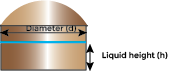
\includegraphics[scale=1]{DigesterWOCDimensions_1}
\end{center}

{
$=\dfrac
	{
		12,000
		\dfrac
			{
			ft^3 \enspace sludge
			}
			{
			day
			}
		*7.48 \dfrac
				{
				gal
				}
				{
				ft^3
				}	
		*(8.34*0.045*0.70) 
		\dfrac
			{lbs VS}
			{gal \enspace  sludge}
	}
	{
		(	\dfrac
			{
			\pi
			}
			{
			4
			}
			*100^2*20
		)
		ft^3
	}
=\boxed
	{
		0.15 \dfrac
			{
			lbs \enspace VS
			}
			{
			day-ft^3
			}
	}
$}\\

\item How much gas is produced in the above digester in $ft^3$/day if the digested sludge contains 2.5\% total solids of which 59\% is volatile solids and the gas production rate is 14 $ft^3$/lb VS destroyed?\\
Solution:\\

{
$
Digester \enspace VS \enspace reduction (\%)=
	\dfrac
	{0.70 - .59}
	{0.70 - 0.70 *0.59}
	*100=38.3\%
$
}\\
\vspace{6mm}

{
$
	\dfrac
	{
	lbs \enspace VS \enspace reduction
	}
	{
	day
	}
	=
	\dfrac
	{
	3153 lbs \enspace VS \enspace feed
		*  0.383 \enspace VS \enspace reduction
	}
	{
	day
	}
 	=1,208
	\dfrac
	{
	lbs \enspace VS \enspace reduction
	}
	{
	day 
	}
$
}\\
\vspace{6mm}

{
$
	\dfrac 
	{
	ft^3 gas \enspace produced
	}
	{
	day
	}
	=
	1208 \dfrac
			{
			lbs \enspace VS \enspace reduced
			}
			{
			day
			}
			*
		\dfrac
		{
		14 ft^3 \enspace gas \enspace produced
		}
		{
		lb \enspace VS \enspace reduced
		}
		=16,912 \dfrac
				{
				ft^3 \enspace digester \enspace 					gas \enspace produced
				}
				{
				day
				}
$
} 
\item The sludge feed to a digester is 80,000 gal/day. The sludge contains 4.5\% total solids with 75\% volatile solids. If 50\% of VS are reduced in the digester: 



\begin{enumerate}
\item Find lbs VS destroyed per 1000 gal of digester capacity per day if the digester radius is 55 ft with an operating sludge level of 25 ft.(5 points)

\vspace{1cm}
Solution:\\
Digester Volume: 
$
{
		(\pi*55^2*25)ft^3 *7.48 \dfrac{gal}{ft^3}
	}=1,776,220 gallons=1,776.2 \enspace(1000 \enspace gallons)
$
\\
\vspace{3mm}
$
	\dfrac
	{
	lbs \enspace VS \enspace reduction
	}
	{
	day
	}
	=
	\dfrac
	{
	80,000 gal * 8.34 \dfrac{lbs}{gal}*(0.045*0.75) \dfrac{lbs VS}{lb}*0.5\dfrac{lbs \enspace VS \enspace  reduction}{lb \enspace VS}
	}
	{
	day
	}$\\
\vspace{0.25cm}
$
 	=11,259
	\dfrac
	{
	lbs \enspace VS \enspace reduction
	}
	{
	day 
	}
$
\\
\vspace{3mm}


$
	\dfrac
	{
	lbs \enspace VS \enspace reduction
	}
	{
	1000 \enspace digester \enspace capacity
	}
	=
	\dfrac
	{
	11,259 \dfrac
			{
			lbs \enspace VS \enspace reduction
			}
			{
			day
			}
	}
	{	
	1,776.2 \enspace (1000 \enspace gallons)
	}
 	=\boxed{6.3
	\dfrac
	{
	lbs \enspace VS \enspace reduction
	}
	{
	1000 gallons \enspace digester \enspace volume 
	}}
$
\\

\vspace{1cm}

\item  What is the digester gas production in Btu/day? Assume 14 cu. ft digester gas per lb of VS destroyed and a 650 Btu/cu. ft heating value for the digester gas produced (5 points)
\end{enumerate}
\vspace{1cm}
Solution:\\

$
	\dfrac 
	{
	ft^3 gas \enspace produced
	}
	{
	day
	}
	=
	11,259 \dfrac
			{
			lbs \enspace VS \enspace reduced
			}
			{
			day
			}
			*
		\dfrac
		{
		14 ft^3 \enspace gas \enspace produced
		}
		{
		lb \enspace VS \enspace reduced
		}
		=157,626 \dfrac
				{
				ft^3 \enspace digester \enspace 					gas \enspace produced
				}
				{
				day
				}
$
\\
\vspace{1cm}


$
	\dfrac 
	{
	BTU \enspace produced
	}
	{
	day
	}
	=
	157,626 \dfrac
			{
			ft^3 \enspace gas \enspace produced
			}
			{
			day
			}
			*
		\dfrac
		{
		650 BTU \enspace gas \enspace produced
		}
		{
		ft^3 gas
		}
		=\boxed{102,456,900 \dfrac
				{
				BTU \enspace produced
				}
				{
				day
				}}
$

\item Two sludges are blended together as follows: 15,000 gal. primary sludge at 4.1\% solids. 28,000 gal. secondary sludge at 1.3\% solids. What is the combined solids concentration?  If the primary sludge is 68\% VS and the secondary sludge is 63\% VS, what is the VS concentration (\%) in the combined sludge?

Solution:

Combined solids concentration:
$
C_1*V_1 + C_2*V_2 = C_3*V_3$\\
$\implies C_3 = \dfrac{C_1*V_1 + C_2*V_2}{V3}=\dfrac{C_1*V_1 + C_2*V_2}{V_1 + V_2}=\dfrac{4.1*15,000 + 1.3*28,000}{15,000 + 28,000}=\boxed{2.28\%}
$\\
Lbs of VS in combined sludge:
$
C\textsubscript{VS1}*V_1 + C\textsubscript{VS2}*V_2 = C\textsubscript{VS3}*V_3$\\
$\implies C\textsubscript{VS3} = \dfrac{C\textsubscript{VS1}*V_1 + C\textsubscript{VS2}*V_2}{V3}=\dfrac{C\textsubscript{VS1}*V_1 + C\textsubscript{VS1}*V_2}{V_1 + V_2}$\\
$\implies C\textsubscript{VS3}
=\dfrac{4.1*15,000*0.68 + 1.3*28,000*0.63}{15,000 + 28,000}=\boxed{1.50\%}$
\\

\pagebreak
	
\item 10,000 gallons of sludge is pumped to an anaerobic digester/day at 4\% solids (70\% VS).  50\% of the VS are destroyed, creating 15 $ft^3$ of gas per lbs. of VS destroyed. How much gas is produced each day?\\

{
$
	\dfrac
	{
	lbs \enspace VS \enspace reduction
	}
	{
	day
	}
	=
	\dfrac
	{
	10,000 gal * 8.34 \dfrac{lbs}{gal}*(0.04*0.7) \dfrac{lbs VS}{lb}*\dfrac{0.5 lbs \enspace VS \enspace  reduction}{lb \enspace VS}
	}
	{
	day
	}
 	=1,168
	\dfrac
	{
	lbs \enspace VS \enspace reduction
	}
	{
	day 
	}
$
}\\
\vspace{3mm}

{
$
	\dfrac 
	{
	ft^3 gas \enspace produced
	}
	{
	day
	}
	=
	1,168 \dfrac
			{
			lbs \enspace VS \enspace reduced
			}
			{
			day
			}
			*
		\dfrac
		{
		15 ft^3 \enspace gas \enspace produced
		}
		{
		lb \enspace VS \enspace reduced
		}
		=17,520 \dfrac
				{
				ft^3 \enspace digester \enspace 					gas \enspace produced
				}
				{
				day
				}
$
} 

\item Two sludges are blended together as follows: 60,000 gal per day. primary sludge at 4.5\% solids and 28,000 gal secondary sludge at 5\% solids. 
\begin{enumerate}
\item What is the combined solids concentration?  (3 points)\\

$\dfrac{60,000*4.5+28,000*5}{88,000}=\boxed{4.66\%}$\\
\vspace{2cm}
\item How many lbs of solids (per day) are in the combined sludge (3 points)\\

$88,000 gal*8.34*0.0466 = \boxed{34,200 lbs}$\\
\vspace{2cm}


\item If the primary sludge is 68\% VS and the secondary sludge is 83\% VS, how many pounds of VS are in the combined sludge? (3 points)\\
$60,000 gal *\dfrac{8.34*0.045*0.68lbs \enspace VS}{gal}+28,000 gal *\dfrac{8.34*0.05*0.83lbs \enspace VS}{gal}=\boxed{25,003 lbs \enspace VS}$
\vspace{2cm}

\item What is the digester feed VS\%?  (3 points)\\
$\dfrac{25,003 lbs \enspace VS}{34,200 lbs TS}=\boxed{73.1\%}$

\vspace{2cm}



\item If the digester is 120’ diameter with a liquid height of 20’, what is the VS loading in lbs VS/ft3-day (3 points)\\

$\dfrac{25,003 lbs \enspace VS}{0.785*120^2*20}=\boxed{\dfrac{0.11 lbs \enspace VS}{day-ft^3}}$\\
\vspace{2cm}





\item If the digested sludge has 52\% VS, calculate the digester VS reduction percent (3 points)\\

$
Digester \enspace VS \enspace reduction (\%)=
	\dfrac
	{0.731 - .52}
	{0.731 - 0.731 *0.52}
	*100=\boxed{60.1\%}
$\\
\vspace{2cm}

\item What is the gas production (ft$^3$/day) if the digester produces 14 ft$^3$ gas/lb VS destroyed (3 points)\\
25,003*0.601$\dfrac{lbs\enspace VS destroyed}{}*\dfrac{14ft^3 \enspace gas \enspace produced}{lb \enspace VS \enspace destroyed}=\boxed{210,375ft^3 gas}$
\\
\vspace{2cm}

\item How many belt presses are needed to keep up with the digested sludge flow if the belt presses can be operated at a maximum flow of 50 GPM (3 points)\\

88,000$\dfrac{gal \enspace sludge}{day}*\dfrac{day}{1440min}=61 GPM$\\
@50 GPM per press - $\boxed{2 \enspace BFP \enspace required}$
\vspace{2cm}
\item If the digested sludge feed to the belt filter presses is 2.6\% and assuming the belt press feed solids capture is 90\%.  How many lbs of solids (dry) are produced by the BFP (4 points)\\
$88,000\dfrac{gal}{day}*8.34*0.026\dfrac{lbs \enspace solids \enspace feed}{day}*0.9\dfrac{lbs \enspace solids \enspace captured}{lbs \enspace solids \enspace feed}=\boxed{17,174 lbs \enspace solids \enspace per \enspace day}$
\vspace{2cm}

\item If the BFP produces a 20\% cake, how many wet tons cake produced per day (4 points)\\
$\dfrac{17,174 lbs \enspace solids \enspace produced}{day}*\dfrac{100 lbs \enspace cake}{20 lbs \enspace solids \enspace produced}*\dfrac{tons}{2,000 lbs}=\boxed{\dfrac{42.9tons}{day}}$
\vspace{2cm}

\item If the cake density is 68 lbs/cu. ft, how much time will it take to fill a 30 cu. yd bin (3 points)\\
(Ans. 15.4 hours)
$\dfrac{(42.9*2000)lbs \enspace cake}{day}*\dfrac{day}{1440 min}=\dfrac{59.583}{lbs \enspace cake}{min}$\\
$\dfrac{59.583}{lbs \enspace cake}{min}*\dfrac{ft^3}{68 lbs \enspace cake}=\dfrac{0.876ft^3}{min}$\\
$30yd^3*\dfrac{27ft^3}{yd^3}*\dfrac{min}{0.876ft^3}*\dfrac{hrs}{60 min}=\boxed{15.4hrs}$
\vspace{2cm}
\item What will be the cost of hauling dewatered cake per day @ \$65 per ton cake (2 points)\\
42.9$\dfrac{tons}{day}*\dfrac{\$65}{ton}=\boxed{\dfrac{\$2,789}{day}}$ 
\end{enumerate}

\item Calculate the VS loading to the digester in lbs/day if 25,000 gallons of sludge containing 4.5\% TS with and average VS content of 76\% is fed to the digester 

Solution:\\
$\dfrac{25,000 \enspace Gal}{day}*\dfrac{8.34 \enspace lbs \enspace sludge}{Gal}* \dfrac{(0.045*0.76) \enspace lbs \enspace VS \enspace feed}{lb \enspace sludge}=\boxed{\dfrac{7,131 \enspace lbs \enspace VS }{day} } $

\item Calculate the organic loading rate to two 320,000 gallon anaerobic digesters given:
Primary sludge feed rate of 25,000 gallons with 6.2\% TS containing 73\% solids and SG of 1.03.
Secondary sludge feed rate of 30,500 gallons with 3.8\% TS containing 77\% solids (7 points)
(Answer: 0.2lbs VS/day-ft3 ) 

\item 10,000 gallons/day of sludge is pumped to an anaerobic digester/day at 4\% solids (70\% VS).  If 50\% of the VS is destroyed, how many lbs of VS is destroyed per day?\\
Solution:\\
$\dfrac{10,000 \enspace Gal}{day}*\dfrac{8.34 \enspace lbs \enspace sludge}{Gal} \dfrac{0.04*0.7 \enspace lbs \enspace VS \enspace feed}{lb \enspace sludge}*\dfrac{0.5 \enspace lbs \enspace VS \enspace destroyed}{lbs \enspace VS \enspace feed}=\boxed{\dfrac{1,168lbs \enspace VS \enspace destroyed}{day} } $

\item  Two sludges are blended together as follows: 8,000 cu. ft primary sludge at 4.90\% solids and 23,000 gal. secondary sludge at 5.20\% solids. What is the combined solids concentration?\\


a. 3.84 \\
b. 6.23 \\
c. 5.12 \\
*d. 4.98 \\

\item  Calculate the VS loading to the digester in lbs/day if 10,000 cu. ft of sludge containing 4.8\% TS with and an average VS content of 82\% (Ans: 24,554)\\

\item  Calculate the VS loading to the digester in lbs/day if 25,000 gallons of sludge containing 4.5\% TS with and average VS content of 76\% is fed to the digester (Ans: 7,131)\\

\item  Calculate the \% VS reduction in a digester given the volatile solids content of the feed sludge to the digester is 76\% and the volatile solids content of the sludge leaving the digester is 55\% (Ans: 61.4)\\

\item  If an anaerobic digester receives sludge with VS of 76\% and discharges digested sludge with a 56\% VS.  Its VS reduction is:\\

a. 36\% \\
b. 48\% \\
*c. 60\% \\
d. 89\% \\

\item  Calculate the VS loading to the digester in lbs/day if 25,000 gallons of sludge containing 4.5\% TS with and average VS content of 76\% is fed to the digester \\

Correct Answer(s):
a. 7131.0 \\

\item  Calculate the organic loading rate to two 320,000 gallon anaerobic digesters given:
Primary sludge feed rate of 25,000 gallons with 6.2\% TS containing 73\% solids and SG of 1.03.
Secondary sludge feed rate of 30,500 gallons with 3.8\% TS containing 77\% solids (7 points)
(Answer: 0.2lbs VS/day-ft3 ) \\

Correct Answer(s): \\


\item  Calculate the VS loading to the digester in lbs/day if 25,000 gallons of sludge containing 4.5\% TS with and average VS content of 76\% is fed to the digester \\

*a. 7,131 lbs/day \\
b. 17,432 lbs/day \\
c. 19,256 lbs/day \\
d. 26,244 lbs/day \\

\item  What is the digester efficiency if the volatile solids concentration entering an anaerobic digester is 70\% and the volatile solids concentration leaving the digester is 50\%? \\

*a. 29\% \\
b. 40\% \\
c. 57\% \\
d. 71\% \\

\item  You are operating a 1 MGD trickling filter plant with a single stage anaerobic digester You pump about 3,000 gpd of sludge to the fixed cover digester.  The supernatant has a BOD of 950 mg/l The BOD loading coming from the supernatant in pounds per day is \\

a. 12 \\
*b. 24 \\
c. 36 \\
d. 48 \\

\item  How many pounds of solids are pumped to a digester each day, if the digester receives 10,000 gpd of sludge at 5\% density? \\

a. 417 lbs/day \\
b. 1,497 lbs/day \\
c. 2,337 lbs/day \\
d. 3,273 lbs/day \\
*e. 4,170 lbs/day \\

\item  If a digester loading is 0.05 lbs VSS/ft3/Day, how large must the digester be if it receives 1,000 lbs. of suspended solids per day with a volatile percentage of 75\%? \\

a. 3,750 cu.ft \\
b. 10,000 cu.ft \\
*c. 15,000 cu.ft \\
d. 26,666 cu.ft \\
e. 37,500 cu.ft \\

\item  What is the digester efficiency if the volatile solids concentration entering an anaerobic digester is 70\% and the volatile solids concentration leaving the digester is 50\%? \\

*a. 29\% \\
b. 40\% \\
c. 57\% \\
d. 71\% \\

\item  You are operating a 1 MGD trickling filter plant with a single stage anaerobic digester You pump about 3,000 gpd of sludge to the fixed cover digester.  The supernatant has a BOD of 950 mg/l The BOD loading coming from the supernatant in pounds per day is \\

a. 12 \\
*b. 24 \\
c. 36 \\
d. 48 \\

\item  How many pounds of solids are pumped to a digester each day, if the digester receives 10,000 gpd of sludge at 5\% density? \\

a. 417 lbs/day \\
b. 1,497 lbs/day \\
c. 2,337 lbs/day \\
d. 3,273 lbs/day \\
*e. 4,170 lbs/day \\


\item  If a digester loading is 0.05 lbs VSS/ft3/Day, how large must the digester be if it receives 1,000 lbs. of suspended solids per day with a volatile percentage of 75\%? \\

a. 3,750 cu.ft \\
b. 10,000 cu.ft \\
*c. 15,000 cu.ft \\
d. 26,666 cu.ft \\
e. 37,500 cu.ft \\

\end{enumerate}

\section*{Disinfection Math Problems}
\begin{enumerate}
\item What is the chlorine demand if the chlorine dosage is 15 mg/l and the residual is 3 mg/l?
Solution:\\
Chlorine dosage = chlorine demand + chlorine residual\\
$\implies chlorine \enspace demand = chlorine \enspace dosage - chlorine \enspace residual=15-3=\boxed{12mg/l}$
\vspace{0.25cm}
\item Calculate how many pounds per day of chlorine should be used to maintain a dosage of 12 mg/l at a 5.0 MGD flow.\\
Solution:\\
$lbs/day=conc. (mg/l)*flow(MGD)*8.34$\\
$lbs/day=12*5*8.34=\boxed{500.4lbs/day}$\\
\vspace{0.25cm}
\item If 80 pounds of chlorine are applied each day to a flow of 1.5 MGD, what is the dosage in mg/l?\\
\vspace{0.25cm}
Solution:\\
\vspace{0.25cm}
Applying the pounds formula:\\  $lbs/day=conc. (mg/l)*flow(MGD)*8.34$\\
\vspace{0.25cm}
$\implies conc. (mg/l)=\frac{lbs/day}{flow(MGD)*8.34}=\frac{80}{1.5*8.34}=\boxed{6.4mg/l}$
\vspace{0.25cm}
\item How many pounds per day of chlorine will be required to disinfect a secondary effluent flow of 1.68 MGD if the chlorine demand is found to be 8.5 mg/l and a residual of 3 mg/l is desired?\\
\vspace{0.25cm}
Chlorine dosage = chlorine demand + chlorine residual\\
\vspace{0.25cm}
$chlorine \enspace dosage=8.5+3=11.5mg/l$\\
$lbs/day=conc. (mg/l)*flow(MGD)*8.34=1.68*11.5*8.34=\boxed{161.2lbs/day}$\\
\vspace{0.25cm}
\item The chlorine demand is 4.8 mg/l and a chlorine residual is 0.75 mg/l is desired. For a flow of 2.8 MGD, how many pounds per day should the chlorinator be set to deliver.\\
Solution:\\
Chlorine dosage = chlorine demand + chlorine residual\\
\vspace{0.25cm}
$chlorine \enspace dosage=4.8+0.75=5.55mg/l$\\
\vspace{0.25cm}
To calculate pounds per day, applying the pounds formula:\\ 
\vspace{0.25cm}
$lbs/day=conc. (mg/l)*flow(MGD)*8.34=2.8*5.55*8.34=\boxed{129.6lbs/day}$\\
\vspace{0.25cm}
\item Chlorine is being fed at the rate of 75 pounds per day. Plant flow is 1.2 MGD. The chlorine residual is measured and found to be 2.6 mg/l Calculate chlorine demand.\\
a. 4.9 mg/l \\
b. 5.7 mg/l \\
c. 7.5 mg/l \\
d. 8.3 mg/l \\
\vspace{0.25cm}
Solution:\\
$Chlorine \enspace dosage (lbs/day)=conc. (mg/l)*flow(MGD)*8.34$\\
$\implies chlorine \enspace dosage \enspace conc. (mg/l)=\frac{lbs/day}{flow(MGD)*8.34}=\frac{75}{1.2*8.34}=7.5mg/l$\\
Chlorine dosage = chlorine demand + chlorine residual\\
\vspace{0.25cm}
$ \implies chlorine \enspace demand = chlorine \enspace dosage - chlorine \enspace residual=7.5-2.6=\boxed{4.9mg/l}$
\vspace{0.25cm}
\item Experience has shown that a minimum dosage of 24 mg/l is necessary in order to disinfect a wastewater effluent and leave a residual of 1.0 mg/l. How many pounds of chlorine must be fed at this dosage to a flow of 0.5 MGD?\\
Prior to sand filtration, a secondary effluent flow of 5 MGD
Solution:\\
Prior to sand filtration, a secondary effluent flow of 5 MGD
$Chlorine \enspace dosage (lbs/day)=conc. (mg/l)*flow(MGD)*8.34=24*0.5*8.34=\boxed{100lbs/day}$\\
\item 25 lbs/day of chlorine is being applied to a wastewater effluent flow of 250,000 gpd. Calculate the chlorine dosage in mg/l.\\
Solution:\\
$lbs/day=conc. (mg/l)*flow(MGD)*8.34$\\
$\implies conc. (mg/l)=\frac{lbs/day}{flow(MGD)*8.34}=\frac{25}{0.25*8.34}=\boxed{12mg/l}$
\item You wish to dose the influent channel at 5 mg/l chlorine to help control odors. The flow is 11.5 MGD.. How many pounds of chlorine must be fed each day? Is it necessary to maintain a chlorine residual to control odors?\\
Solution:\\
$lbs/day=conc. (mg/l)*flow(MGD)*8.34=5*11.5*8.34=\boxed{480lbs/day}$\\
No.  Chlorine residual is for disinfection only.  Odor control would not require a residual\\
\item Jar testing shows that the chlorine demand of an effluent is 12.5 mg/l. In order to assure disinfection, a residual of 1.0 mg/l is required. How many pounds of chlorine must be fed per 1MGD to assure disinfection?\\
Solution: 
$ chlorine \enspace dosage = chlorine \enspace demand \enspace + \enspace chlorine \enspace residual$\\
$\implies chlorine \enspace dosage = (12.5 \enspace + \enspace 1 )mg/l=13.5 mg/l$\\
$lbs/day=13.5(mg/l)*1(MGD)*8.34=\boxed{112.6 lbs/day}$
\item What is the chlorine dosage if the chlorinator is feeding 120 lbs/day and the average daily flow is 3.5 MGD?  What is the chlorine demand if the residual is 1.3 mg/l?\\
Solution:\\
a. $Chlorine \enspace dosage (lbs/day)=conc. (mg/l)*flow(MGD)*8.34$\\
$\implies chlorine \enspace dosage \enspace conc. (mg/l)=\frac{lbs/day}{flow(MGD)*8.34}=\frac{120}{3.5*8.34}=\boxed{4.1mg/l}$\\
b. Chlorine dosage = chlorine demand + chlorine residual\\
$ \implies chlorine \enspace demand = chlorine \enspace dosage - chlorine \enspace residual=4.1-1.3=\boxed{2.8mg/l}$

\item Experience has shown that a minimum dosage of 24 mg/l is necessary in order to disinfect a wastewater effluent and leave a residual of 1.0 mg/l. How many pounds of chlorine must be fed at this dosage to a flow of 0.5 MGD?\\
Solution:\\
$Chlorine \enspace dosage (lbs/day)=conc. (mg/l)*flow(MGD)*8.34=24*0.5*8.34=\boxed{100lbs/day}$\\
\vspace{0.25cm}
\item 25 lbs/day of chlorine is being applied to a wastewater effluent flow of 250,000 gpd. Calculate the chlorine dosage in mg/l.\\
Solution:\\
$lbs/day=conc. (mg/l)*flow(MGD)*8.34$\\
$\implies conc. (mg/l)=\frac{lbs/day}{flow(MGD)*8.34}=\frac{25}{0.25*8.34}=\boxed{12mg/l}$
\vspace{0.25cm}
\item You wish to dose the influent channel at 5 mg/l chlorine to help control odors. The flow is 11.5 MGD.. How many pounds of chlorine must be fed each day? Is it necessary to maintain a chlorine residual to control odors?\\
Solution:\\
$lbs/day=conc. (mg/l)*flow(MGD)*8.34=5*11.5*8.34=\boxed{480lbs/day}$\\
No.  Chlorine residual is for disinfection only.  Odor control would not require a residual\\
\item Jar testing shows that the chlorine demand of an effluent is 12.5 mg/l. In order to assure disinfection, a residual of 1.0 mg/l is required. How many pounds of chlorine must be fed per 1MGD to assure disinfection?\\
Solution: 
$ chlorine \enspace dosage = chlorine \enspace demand \enspace + \enspace chlorine \enspace residual$\\
$\implies chlorine \enspace dosage = (12.5 \enspace + \enspace 1 )mg/l=13.5 mg/l$\\
$lbs/day=13.5(mg/l)*1(MGD)*8.34=\boxed{112.6 lbs/day}$
\item What is the chlorine dosage if the chlorinator is feeding 120 lbs/day and the average daily flow is 3.5 MGD?  What is the chlorine demand if the residual is 1.3 mg/l?\\
\vspace{0.25cm}
Solution:\\
a. $Chlorine \enspace dosage (lbs/day)=conc. (mg/l)*flow(MGD)*8.34$\\
$\implies chlorine \enspace dosage \enspace conc. (mg/l)=\frac{lbs/day}{flow(MGD)*8.34}=\frac{120}{3.5*8.34}=\boxed{4.1mg/l}$\\
b. Chlorine dosage = chlorine demand + chlorine residual\\
$ \implies chlorine \enspace demand = chlorine \enspace dosage - chlorine \enspace residual=4.1-1.3=\boxed{2.8mg/l}$
\vspace{0.25cm}
\item A 2.5 MGD secondary flow is disinfected by the application of 320 lbs of chlorine per day.  This dose provides a chemical residual of 2.1 mg/l.  There is a need to switch to the use of sodium hypochlorite which has a 12.5\% available chlorine, SG of 1.2 and a cost of \$0.60 per gallon. Chlorine costs \$0.28/lb.\\ Calculate: 1) The chlorine demand, and 2) Cost difference (\$ per day) between chlorine and sodium hypochlorite\\
\vspace{0.25cm}
Dosage = Demand + Residual\\
\vspace{0.25cm}
\textbf{Dosage:}\\
\vspace{0.25cm}
$\dfrac{320 lbs \enspace chlorine}{day}=2.5 MGD * 8.34 * x \dfrac{mg}{l}$\\
\vspace{0.25cm}
$x \dfrac{mg}{l}=\dfrac{320}{2.5*8.34}=15.34\dfrac{mg}{l}$\\
\vspace{0.25cm}
Chlorine Demand = Dosage - Residual = 15.34 - 2.1 = $\boxed{13.24\dfrac{mg}{l}}$\\
\vspace{0.25cm}
Cost per day to use chlorine: $\dfrac{\$320}{lb}*\dfrac{\$0.28}{lb}=\$89.60$\\
\vspace{0.25cm}
To calculate the hypochlorite we need to determine the gallons per day of bleach required.\\
\vspace{0.25cm}
$320 \dfrac{lbs \enspace chlorine}{day}\enspace=\enspace x \dfrac{gal \enspace bleach}{day} \enspace * \enspace 8.34 * 1.2 \dfrac{lbs \enspace bleach}{per \enspace gal \enspace bleach}* \enspace 0.125 \dfrac{lbs \enspace chlorine}{lb \enspace bleach}$\\
\vspace{0.25cm}
$ \rightarrow x \dfrac{gal \enspace bleach}{day}\enspace = \enspace \dfrac{320}{8.34*1.2*0.125} \enspace = \enspace 256 \dfrac{gal \enspace bleach}{day}$\\
\vspace{0.25cm}
$\enspace 256 \dfrac{gal \enspace bleach}{day}*\dfrac{\$0.60}{gal \enspace bleach}=\$153.48$
\vspace{0.25cm}
Cost difference \$153.48 - \$89.60 = $\boxed{\$63.88}$
\vspace{0.25cm}
\item Three hundred pounds (300 lbs) per day of chlorine (cost = \$0.32/lb) are being used to  disinfect  a secondary  effluent flow of 6.5 MGD.  Due to  safety concerns, the substitution of sodium hypochlorite (12.5\% available chlorine, 10.0 lbs/gal and a cost of \$0.55/gal) for the chlorine  is being considered  at  this plant. What is the cost difference per day between the chlorine and sodium hypochlorite?\\
\vspace{0.25cm}
 (Ans:\$36/year)

\item The operator at a 1.5 MGD conventional activated sludge plant is considering using either HTH or sodium hypochlorite as an alternative to chlorine gas. Currently chlorine is being dosed at 15 mg/l in order to achieve a residual of 3.0 mg/l. Using the data provided below calculate the daily cost for chlorine, HTH, and sodium hypochlorite (NaOCl) (Sp.Gravity 1.21).
 
Chlorine $\rightarrow$ 0.15 \$/lb\\
HTH (70\% available chlorine) $\rightarrow$ 0.25 \$/lb\\
NaOCl (15\% available chlorine) $\rightarrow$ 0.35 \$/gal                                                        

\vspace{0.25cm}
\textbf{SOLUTION}\\
\textbf{lbs chlorine required:}\\
$\dfrac{1.5 MG}{day}*\dfrac{8.34lbs}{gallon}*\dfrac{15mg \enspace chlorine}{l}=\dfrac{188 lbs \enspace chlorine}{day}$\\
\vspace{0.25cm}
\textbf{Daily cost if chlorine is used:}\\
$188lbs \enspace chlorine*\dfrac{\$0.15}{lb \enspace chlorine}=\boxed{\$28.20}$\\
\vspace{0.25cm}
\textbf{Daily cost if HTH is used:}\\
$188lbs \enspace chlorine*\dfrac{lb \enspace HTH}{0.7lb \enspace chlorine}*\dfrac{\$0.25}{lb \enspace chlorine}=\boxed{\$67.14}$\\
\vspace{0.25cm}
\textbf{Daily cost if NaOCl is used:}\\
$188lbs \enspace chlorine*\dfrac{lb \enspace NaOCl}{0.15lb \enspace chlorine}*\dfrac{gal \enspace NaOCl}{8.34*1.21 lbs\enspace NaOCl}*\dfrac{\$0.35}{gal \enspace NaOCl}=\boxed{\$43.47}$
\pagebreak
\item A water storage tank is 30 feet in diameter and has a water depth of 18.5 feet. It is desired to super-chlorinate this tank with 30 ppm of chlorine, how many pounds of HTH will be required (HTH has 70\% available chlorine)?\\    
\vspace{0.25cm}
\textbf{Tank Volume:}\\
$0.785*30^2*18.5ft^3*7.48\dfrac{gal}{ft^3}=97,765 gal$\\
\vspace{0.25cm}
\textbf{lbs HTH required:}\\
$\dfrac{30lbs \enspace chlorine}{1,000,000lbs  \enspace water}*\dfrac{8.34lbs \enspace water}{gal \enspace water}*97,765 gal \enspace water *\dfrac{lb \enspace HTH}{0.70lb \enspace chlroine}=\boxed{35 lbs \enspace HTH}$
\vspace{0.25cm}
\item The chlorine demand is 4.8 mg/l and a chlorine residual is 0.75 mg/l is desired.  For a flow of 2.8 MGD, how many pounds per day should the chlorinator be set to deliver.\\
*a. 130 \\
b. 116 \\
c. 112 \\
d. 18 \\
e. 16 \\
\item Chlorine is being fed at the rate of 75 pounds per day. Plant flow is 1.2 MGD. The chlorine residual is measured and found to be 2.6 mg/l Calculate chlorine demand.\\
*a. 4.9 mg/l \\
b. 5.7 mg/l \\
c. 7.5 mg/l \\
d. 8.3 mg/l \\
\item Assuming that a chlorine residual of 0.5 mg/l is being maintained and the chlorine demand is 19.5 mg/l, approximately how many pounds of chlorine per day will be required to treat a flow of 5.0 MGD?\\
a. 21 lbs \\
b. 792 lbs \\
c. 813 lbs \\
*d. 834 lbs \\
\item Chlorine is being fed at the rate of 75 pounds per day. Plant flow is 1.2 MGD. The chlorine residual is measured and found to be 2.6 mg/l Calculate chlorine demand.\\
*a. 4.9 mg/l \\
b. 5.7 mg/l \\
c. 7.5 mg/l \\
d. 8.3 mg/l \\
\item If 25 Ibs/day of chlorine is being applied to a wastewater effluent flow of 250,000 gpd. Calculate the chlorine demand in mg/l if the chlorine residue is 1.2 mg/l.\\
a. 2.5 mg/l \\
*b. 10.8 mg/l \\
c. 15.1 mg/l \\
d. 6.3 mg/l \\
\item Calculate how many pounds per day of chlorine should be used to maintain a dosage of 12 mg/l at 6.0 MGD flow\\
a. 60 lbs/day \\
b. 450 lbs/day \\
c. 500 lbs/day \\
*d. 600 lbs/day \\
e. 6,700 lbs/day \\
\item Chlorine is being fed at the rate of 75 pounds per day. Plant flow is 1.2 MGD. The chlorine residual is measured and found to be 2.6 mg/l Calculate chlorine demand. \\
*a. 4.9 mg/l \\
b. 5.7 mg/l \\
c. 7.5 mg/l \\
d. 8.3 mg/l \\
\item Chlorine is being fed at the rate of 200 pounds per day. Plant flow is 4 MGD. The chlorine residual is measured and found to be 3 mg/l Calculate chlorine demand. \\
a. 3 mg/l \\
*b. 2 mg/l \\
c. 16 mg/l \\
d. 9 mg/l \\
\item The chlorine demand is 4.8 mg/l and a chlorine residual is 0.75 mg/l is desired.  For a flow of 2.8 MGD, how many pounds per day should the chlorinator be set to deliver. \\
*a. 130 \\
b. 116 \\
c. 112 \\
d. 18 \\
e. 16 \\
\item Chlorine is being fed at the rate of 75 pounds per day. Plant flow is 1.2 MGD. The chlorine residual is measured and found to be 2.6 mg/l Calculate chlorine demand. \\
*a. 4.9 mg/l \\
b. 5.7 mg/l \\
c. 7.5 mg/l \\
d. 8.3 mg/l \\
\item Assuming that a chlorine residual of 0.5 mg/l is being maintained and the chlorine demand is 19.5 mg/l, approximately how many pounds of chlorine per day will be required to treat a flow of 5.0 MGD? \\
a. 21 lbs \\
b. 792 lbs \\
c. 813 lbs \\
*d. 834 lbs \\
\item Chlorine is being fed at the rate of 75 pounds per day. Plant flow is 1.2 MGD. The chlorine residual is measured and found to be 2.6 mg/l Calculate chlorine demand. \\
*a. 4.9 mg/l \\
b. 5.7 mg/l \\
c. 7.5 mg/l \\
d. 8.3 mg/l \\
\item If 25 Ibs/day of chlorine is being applied to a wastewater effluent flow of 250,000 gpd. Calculate the chlorine demand in mg/l if the chlorine residue is 1.2 mg/l. \\
a. 2.5 mg/l \\
*b. 10.8 mg/l \\
c. 15.1 mg/l \\
d. 6.3 mg/l \\
\item Calculate how many pounds per day of chlorine should be used to maintain a dosage of 12 mg/l at 6.0 MGD flow \\
a. 60 lbs/day \\
b. 450 lbs/day \\
c. 500 lbs/day \\
*d. 600 lbs/day \\
e. 6,700 lbs/day \\
\item What is the chlorine residual of a 2.5 MGD secondary effluent stream if its chlorine demand is 9 mg/l and is treated with 300 lbs/day chlorine?   Ans:  5.4
\\
\item How many lbs per day of chlorine is required to maintain a dosage of 12 mg/l for a 5 MGD flow?   Ans:  500.4
\\
\item What is the chlorine residual of a 2.5 MGD secondary effluent stream if its chlorine demand is 9 mg/l and is treated with 300 lbs/day chlorine? Ans:  5.4
\\
\item How many lbs per day of chlorine is required to maintain a dosage of 12 mg/l for a 5 MGD flow?  Ans:  500.4
\\
\item What is the chlorine residual of a 2.5 MGD secondary effluent  Ans:  5.4
\\
\item How many lbs per day of chlorine is required to maintain a dosage of 12 mg/l for a 5 MGD flow? Ans:  500.4
\\
\item Experience has shown that a minimum dosage of 24 mg/l is necessary in order to disinfect a wastewater effluent and leave a residual of 1.0 mg/l. How many pounds of chlorine must be fed at this dosage to a flow of 0.5 MGD? Ans:  100.0
\\
\item 25 lbs/day of chlorine is being applied to a wastewater effluent ow of 250,000 gpd. Calculate the chlorine dosage in mg/l.  Ans:  12.0
\\
\item You wish to dose the in influent channel at 5 mg/l chlorine to help control odors. The flow is 11.5 MGD.  How many pounds of chlorine must be fed each day? Is it necessary to maintain a chlorine residual to control odors?   Ans:480.0\\
\item Jar testing shows that the chlorine demand of an effluent is 12.5 mg/l. In order to assure disinfection, a residual of 1.0 mg/l is required. How many pounds of chlorine must be fed per 1MGD to assure disinfection?  Ans:  112.6
\\
\item What is the chlorine dosage if the chlorinator is feeding 120 lbs/day and the average daily flow is 3.5 MGD?  Ans:  4.1 \\
\item What is the chlorine residual of a 2.5 MGD secondary effluent stream if its chlorine demand is 9 mg/l and is treated with 300 lbs/day chlorine?  Ans:  5.4
\\
\item How many lbs per day of chlorine is required to maintain a dosage of 12 mg/l for a 5 MGD flow?  Ans:  500.4
\\
\item Chlorine is being fed at the rate of 75 pounds per day. Plant flow is 1.2 MGD. The chlorine residual is measured and found to be 2.6 mg/l Calculate chlorine demand. \\
*a. 4.9 mg/l \\
b. 5.7 mg/l \\
c. 7.5 mg/l \\
d. 8.3 mg/l \\
\item Chlorine is being fed at the rate of 75 pounds per day. Plant flow is 1.2 MGD. The chlorine residual is measured and found to be 2.6 mg/l Calculate chlorine demand. \\
*a. 4.9 mg/l \\
b. 5.7 mg/l \\
c. 7.5 mg/l \\
d. 8.3 mg/l \\
\item Chlorine is being fed at the rate of 200 pounds per day. Plant flow is 4 MGD. The chlorine residual is measured and found to be 3 mg/l Calculate chlorine demand. \\
a. 3 mg/l \\
*b. 2 mg/l \\
c. 16 mg/l \\
d. 9 mg/l \\
\item Chlorine is being fed at the rate of 200 pounds per day. Plant flow is 4 MGD. The chlorine residual is measured and found to be 3 mg/l Calculate chlorine demand. \\
a. 3 mg/l \\
*b. 2 mg/l \\
c. 16 mg/l \\
d. 9 mg/l \\
\item The chlorine demand is 4.8 mg/l and a chlorine residual is 0.75 mg/l is desired.  For a flow of 2.8 MGD, how many pounds per day should the chlorinator be set to deliver. \\
*a. 130 \\
b. 116 \\
c. 112 \\
d. 18 \\
e. 16 \\
\item Chlorine is being fed at the rate of 75 pounds per day. Plant flow is 1.2 MGD. The chlorine residual is measured and found to be 2.6 mg/l Calculate chlorine demand. \\
*a. 4.9 mg/l \\
b. 5.7 mg/l \\
c. 7.5 mg/l \\
d. 8.3 mg/l \\
\item Assuming that a chlorine residual of 0.5 mg/l is being maintained and the chlorine demand is 19.5 mg/l, approximately how many pounds of chlorine per day will be required to treat a flow of 5.0 MGD? \\
a. 21 lbs \\
b. 792 lbs \\
c. 813 lbs \\
*d. 834 lbs \\
\item Chlorine is being fed at the rate of 75 pounds per day. Plant flow is 1.2 MGD. The chlorine residual is measured and found to be 2.6 mg/l Calculate chlorine demand. \\
*a. 4.9 mg/l \\
b. 5.7 mg/l \\
c. 7.5 mg/l \\
d. 8.3 mg/l \\
\item If 25 Ibs/day of chlorine is being applied to a wastewater effluent flow of 250,000 gpd. Calculate the chlorine demand in mg/l if the chlorine residue is 1.2 mg/l. \\
a. 2.5 mg/l \\
*b. 10.8 mg/l \\
c. 15.1 mg/l \\
d. 6.3 mg/l \\
\item Calculate how many pounds per day of chlorine should be used to maintain a dosage of 12 mg/l at 6.0 MGD flow \\
a. 60 lbs/day \\
b. 450 lbs/day \\
c. 500 lbs/day \\
*d. 600 lbs/day \\
e. 6,700 lbs/day \\
\item How many pounds of chlorine will be used in one day if the flow is 700,000 gpd and a uniform dose of 12 mg/l is applied? \\
*a. 7 lbs \\
b. 15 lbs \\
c. 22 lbs \\
d. 26 lbs \\
\item Assuming that a chlorine residual of 0.5 mg/l is being maintained and the chlorine demand is 19.5 mg/l, approximately how many pounds of chlorine per day will be required to treat a flow of 50 MGD? \\
a. 21 lbs \\
b. 792 lbs \\
c. 813 lbs \\
*d. 834 lbs \\
\item How many pounds of chlorine gas is necessary to treat 4,000,000 gallons of wastewater at a dosage of 2 mg/l? \\
a. 61 lbs \\
b. 65 lbs \\
*c. 67 lbs \\
d. 69 lbs \\
\item If you need a chlorine residual of 1 mg/l , how many pounds of chlorine must be applied each day if the fl ow is 2.5 MGD and the chlorine demand is l5 mg/l? \\
a. 291 .pounds/day \\
b. 312 pounds/day \\
*c. 334 pounds/day \\
d. 419 pounds/day \\
e. 516 pounds/day \\
\item Chlorine is being fed at the rate of 75 pounds per day. Plant flow is 1.2 MGD. The chlorine residual is measured and found to be 2.6 mg/l Calculate chlorine demand. \\
*a. 4.9 mg/l \\
b. 5.7 mg/l \\
c. 7.5 mg/l \\
d. 8.3 mg/l \\
\item Chlorine is being fed at the rate of 200 pounds per day. Plant flow is 4 MGD. The chlorine residual is measured and found to be 3 mg/l Calculate chlorine demand. \\
a. 3 mg/l \\
*b. 2 mg/l \\
c. 16 mg/l \\
d. 9 mg/l \\
\item The chlorine demand is 4.8 mg/l and a chlorine residual is 0.75 mg/l is desired.  For a flow of 2.8 MGD, how many pounds per day should the chlorinator be set to deliver. \\
*a. 130 \\
b. 116 \\
c. 112 \\
d. 18 \\
e. 16 \\
\item Chlorine is being fed at the rate of 75 pounds per day. Plant flow is 1.2 MGD. The chlorine residual is measured and found to be 2.6 mg/l Calculate chlorine demand. \\
*a. 4.9 mg/l \\
b. 5.7 mg/l \\
c. 7.5 mg/l \\
d. 8.3 mg/l \\
\item Assuming that a chlorine residual of 0.5 mg/l is being maintained and the chlorine demand is 19.5 mg/l, approximately how many pounds of chlorine per day will be required to treat a flow of 5.0 MGD? \\
a. 21 lbs \\
b. 792 lbs \\
c. 813 lbs \\
*d. 834 lbs \\
\item Chlorine is being fed at the rate of 75 pounds per day. Plant flow is 1.2 MGD. The chlorine residual is measured and found to be 2.6 mg/l Calculate chlorine demand. \\
*a. 4.9 mg/l \\
b. 5.7 mg/l \\
c. 7.5 mg/l \\
d. 8.3 mg/l \\
\item If 25 Ibs/day of chlorine is being applied to a wastewater effluent flow of 250,000 gpd. Calculate the chlorine demand in mg/l if the chlorine residue is 1.2 mg/l. \\
a. 2.5 mg/l \\
*b. 10.8 mg/l \\
c. 15.1 mg/l \\
d. 6.3 mg/l \\
\item Calculate how many pounds per day of chlorine should be used to maintain a dosage of 12 mg/l at 6.0 MGD flow \\
a. 60 lbs/day \\
b. 450 lbs/day \\
c. 500 lbs/day \\
*d. 600 lbs/day \\
e. 6,700 lbs/day \\
\end{enumerate}

\section*{Chemical Dosing Math Problems}

\begin{enumerate}

\item Polymer is being added at 0.2 mg/l in order to achieve a 98\% capture efficiency for a belt press.  The feed to the belt press is 75 gallons per minute, containing 2.5\% solids.  Given the polymer costs \$250 per gallon of 4.5\% active polymer with a specific gravity of 1.08.  What is the cost of polymer per dry ton of solids captured  \\
\vspace{0.25cm}
\textbf{Solution:}\\
\vspace{0.25cm}
\textbf{lbs polymer required:}\\
$75*1440 \dfrac{gal \enspace sludge}{day}* 8.34 \dfrac{lbs \enspace sludge}{gal \enspace sludge} *\dfrac{0.2lbs \enspace polymer}{1,000,000 lbs \enspace sludge}$\\
\vspace{0.25cm}
$= 0.1801 \dfrac{lbs \enspace polymer}{day}$\\

\vspace{0.25cm}
\textbf{gallons polymer solution required:}\\ $0.1801 \dfrac{lbs \enspace polmyer}{day}\enspace=\enspace x \dfrac{gal \enspace polymer \enspace solution}{day} \enspace * \enspace \dfrac{8.34*1.08lbs \enspace polymer \enspace solution}{\enspace gal \enspace polymer \enspace solution}* \enspace 0.045 \dfrac{lbs \enspace polymer}{lb \enspace polymer \enspace solution}$\\
\vspace{0.25cm}
=0.444$\dfrac{gal \enspace polymer \enspace solution}{day}$
\vspace{0.25cm}

\textbf{Polymer cost:}\\
$\dfrac{\$250}{gallon \enspace polymer \enspace soultion}*\dfrac{0.444 gal \enspace polymer \enspace soultion}{day}$\\
\vspace{0.25cm}
=$\dfrac{\$111}{day}$\\
\vspace{0.25cm}
\textbf{Dry tons of solids captured:}\\
$ 75*1440\dfrac{gal \enspace sludge}{day}*\dfrac{8.34*0.025\enspace lbs \enspace solids}{gal \enspace sludge}*\dfrac{0.98\enspace lbs \enspace solids \enspace captured}{lbs \enspace solids}*\dfrac{ton \enspace solids}{2000 lbs \enspace solids}$\\
=$\dfrac{11tons \enspace dry \enspace solids}{day}$\\
\vspace{0.25cm}
\textbf{Polymer cost per dry ton of solids captured:}\\
\vspace{0.25cm}
$\dfrac{\$111 per day}{11 tons \enspace dry \enspace solids \enspace per \enspace day}= \boxed{\$10.09}$

\vspace{0.25cm}
\item A 50 MGD flow is being treated with 20 mg/l ferric chloride.   How many lbs of ferric chloride is required daily \\
\vspace{0.3cm}
\textbf{lbs ferric chloride required:}\\
$\dfrac{50 MG}{day}*\dfrac{8.34lbs}{gallon}*\dfrac{20mg \enspace ferric \enspace chloride}{l}=\boxed{\dfrac{8,340 lbs \enspace ferric \enspace chloride}{day}}$\\
\vspace{0.25cm}
\item If the ferric chloride solution used contains 40\% dry ferric chloride with a specific gravity of 1.4, what is its required feed rate in GPM (7 points)\\
\vspace{0.25cm}
\textbf{Required $FeCl_3$ feed (gal/min) to feed 8,340 lbs ferric chloride:}\\
$\dfrac{8,340 lbs \enspace FeCl_3}{day}=\dfrac{x gal \enspace FeCl_3 \enspace soltn.}{minute}*\dfrac{8.34*1.4 lbs \enspace FeCl_3 \enspace soltn}{gal \enspace FeCl_3 \enspace soltn.}*\dfrac{0.4 lbs \enspace FeCl_3}{lbs \enspace FeCl_3 \enspace soltn.}*\dfrac{1440min}{day}$\\
$\implies x=\dfrac{8,340}{8.34*1.4*0.4*1440}=\boxed{\dfrac{1.24gal}{min}}$\\
\vspace{0.25cm}
\item What is the daily ferric chloride dosing cost if the ferric chloride cost is \$580/dry ton ferric chloride (5 points)\\
\textbf{Daily ferric chloride dosing cost:}\\
\vspace{0.25cm}
$\dfrac{8,340lbs \enspace FeCl_3}{day}*\dfrac{ton}{2000 lbs}*\dfrac{\$580}{ton \enspace FeCl_3}=\boxed{\dfrac{\$2,419}{day}}$
\vspace{0.25cm}
\item A 0.5\% (based on dry weight) solution of polymer is being fed to a secondary effluent prior to sand filtration. It is desired to dose this effluent at 2.5 mg/l. Assuming an effluent flow of 3000 gpm, at what rate (gpm)  should  the polymer feed pump be set?\\	·
\vspace{0.25cm}
\textbf{lbs polymer required:}\\
$\dfrac{3000 gallons}{min}*\dfrac{8.34 \enspace lbs \enspace effluent}{gallon}*\dfrac{2.5 \enspace lbs \enspace polymer}{1,000,000 lbs \enspace effluent}=\dfrac{0.0626 lbs \enspace polymer}{min}$\\
\vspace{0.25cm}
\textbf{Required pumping rate to feed 0.0626 lbs polymer minute:}\\
$\dfrac{0.0626 \enspace lbs \enspace polymer}{min}=\dfrac{x \enspace gallon \enspace polymer  \enspace solution}{minute}*\dfrac{8.34 \enspace lbs \enspace polymer \enspace solution}{gallon \enspace polymer \enspace solution}*\dfrac{0.005 \enspace lbs \enspace polymer}{lbs \enspace polymer \enspace solution}$\\
\vspace{0.25cm}
$\dfrac{x \enspace gallon \enspace polymer solution}{minute}=\dfrac{0.0626}{8.34*0.005}=\boxed{\dfrac{1.5 \enspace gallon}{min}}$\\
\vspace{0.25cm}
\item How many pounds of dry polymer should be added to how many gallons  of water  to make enough 2\% polymer  solution to dose a 10 MGD secondary  effluent flow at 3.0 ppm of polymer?\\
\vspace{0.25cm}
\textbf{lbs polymer required:}\\
$10 MGD*\dfrac{8.34lbs \enspace effluent}{gallon}*\dfrac{3mg \enspace polymer}{l}=\dfrac{250.2 lbs \enspace polymer}{day}$\\
\vspace{0.25cm}
\textbf{Required pumping rate to feed 250.2 lbs polymer minute:}\\
$\dfrac{250.2 lbs \enspace polymer}{day}=\dfrac{x gallon \enspace polymer \enspace solution}{day}*\dfrac{8.34 lbs \enspace polymer \enspace solution}{gallon \enspace polymer \enspace solution}*\dfrac{0.02 lbs \enspace polymer}{lbs \enspace ploymer \enspace solution}$\\

\vspace{0.25cm}
$\dfrac{x gallon \enspace polymer \enspace solution}{day}=\dfrac{250.2}{8.34*0.02}=\boxed{\dfrac{1500 gallon}{day}}$\\
\vspace{0.25cm}
\textbf{This can also be done as follows:}\\
$\dfrac{250.2 lbs \enspace polymer}{day}*\dfrac{lbs \enspace ploymer \enspace solution}{0.02 lbs \enspace polymer}*\dfrac{gallon \enspace polymer \enspace solution}{8.34 lbs \enspace polymer \enspace solution}=\boxed{\dfrac{1500 gallon}{day}}$\\
\vspace{0.25cm}
$\boxed{\textbf{So dissolve 250.2 lbs polymer in 1500 gallons}}$\\
\vspace{0.25cm}
\textbf{Check:}
$\dfrac{250.2lbs \enspace polymer}{1500*8.34 lbs \enspace polymer \enspace solution}=\dfrac{0.02 lbs \enspace polymer}{lb \enspace polymer \enspace solution}=2\% polymer$
\vspace{0.25cm}

\item A 0.35\% solution of polymer is being fed to a secondary effluent prior to sand filtration. The polymer feed pump is set to pump 0.5 gpm to an effluent flow of 4200 gpm. What is the polymer dose rate in ppm?\\
\vspace{0.25cm}
\textbf{Pounds polymer pumped:}\\
$\dfrac{0.5gal \enspace PS}{min}*\dfrac{8.34lbs \enspace PS}{gal \enspace PS}*\dfrac{0.0035lbs \enspace P}{lb \enspace PS}=\dfrac{0.0146lbs \enspace Polymer}{min}$\\
\textbf{Polymer dose rate:}\\
$\dfrac{lbs \enspace polymer}{10^6 \enspace lbs \enspace effluent}(ppm \enspace or \enspace \dfrac{mg}{l})=\dfrac{0.0146lbs \enspace min}{\dfrac{8.34*4,200}{1,000,000}10^6 \enspace lbs \enspace effluent}=\boxed{0.42 ppm \enspace polymer}$
\vspace{0.25cm}
\item Liquid alum (49\% alum, sp. gravity 1.32, \$1.85/gal)) is being used to remove phosphorus from a 600,000 gpd activated sludge effluent. Two hundred milligrams per liter (200 mg/l) of alum, $Al_2(S0_4)_3.14H_20$, is required to give adequate removal of the phosphorus in this effluent. Calculate the daily cost of liquid alum needed to remove phosphorus. [Formula Weights: Al =27, $Al_2(S0_4)_3.14H_20$ =594]\\
\vspace{0.25cm}
\textbf{lbs alum required:}\\
$\dfrac{0.6 MG}{day}*\dfrac{8.34lbs}{gallon}*\dfrac{200mg \enspace alum}{l}=\dfrac{1001 lbs \enspace alum}{day}$\\
\vspace{0.25cm}
\textbf{Required liquid alum feed (gal/day) to feed 1001 lbs alum:}\\
$\dfrac{1001 lbs \enspace alum}{day}=\dfrac{x gallon \enspace liquid \enspace alum}{minute}*\dfrac{8.34*1.32 lbs \enspace liquid \enspace alum}{gallon \enspace liquid \enspace alum}*\dfrac{0.49 lbs \enspace alum}{lbs \enspace liquid \enspace alum}$\\
\vspace{0.25cm}
$\implies x=\dfrac{1001}{8.34*1.32*0.49}=186gal$\\
\vspace{0.25cm}
\textbf{Daily cost of liquid alum to remove phosphorous:}\\
$\dfrac{186gal}{day}*\dfrac{\$1.85}{gal}=\boxed{\dfrac{\$344.10}{day}}$

\vspace{0.25cm}

\item A 1.5\% polymer solution (based on dry weight) is to be fed at the rate of 3.5 pp to a secondary effluent flow of 4.0 MGD.\\
(a) Calculate the polymer pump feed rate (gallon per minute) necessary to dose this secondary effluent. \\
(b) How many gallons per day of polymer solution will be required for an average flow of 3470 gpm?\\ 
\vspace{0.25cm}
(a)
\begin{itemize}
\item \textbf{Polymer required:}\\
$4*3.5*8.34=\dfrac{116.8 lbs \enspace polymer}{day}$\\
\item \textbf{Feed rate ($\dfrac{gal}{min}$):}\\
$\dfrac{116.8lbs \enspace polymer}{day}*
\dfrac{100lbs \enspace polymer \enspace solution}{1.5 lbs polymer}*
\dfrac{gal \enspace polymer \enspace solution}{8.34 lbs \enspace polymer \enspace solution}*
\dfrac{day}{1440min}=\boxed{0.65\dfrac{gal}{min}}$
\end{itemize}
\vspace{0.25cm}
(b)
\begin{itemize}

\item \textbf{Polymer required:}\\
$\bigg[\dfrac{3470gal}{min}*
\dfrac{MG}{1,000,000gal}*
\dfrac{1440min}{day}\bigg]MGD*3.5*8.34=\dfrac{145.9 lbs \enspace polymer}{day}$\\
\item \textbf{Feed rate ($\dfrac{gal}{min}$):}\\
$\dfrac{145.9lbs \enspace polymer}{day}*
\dfrac{100lbs \enspace polymer \enspace solution}{1.5 lbs polymer}*
\dfrac{gal \enspace polymer \enspace solution}{8.34 lbs \enspace polymer \enspace solution}*
\dfrac{day}{1440min}=\boxed{0.81\dfrac{gal}{min}}$
\end{itemize}
\vspace{0.25cm}

\item Liquid alum (Sp. gravity 1.32, 49\% Alum, \$1.70 per gallon,) is being used to remove phosphorus from a 595,000 gal/day secondary. A dose of 14.0 mg/l of aluminum is required to give adequate removal of the phosphorus in this effluent. Calculate the daily cost of liquid alum. (Note: Dry alum contains 9.4\% aluminum).\\
\vspace{0.25cm}
\textbf{Aluminum Required:}\\
$0.595*14*8.34=\dfrac{69.47 lbs \enspace aluminum}{day}$\\
\textbf{Cost of alum ($\dfrac{\$}{day}$):}\\
$\dfrac{69.47lbs \enspace aluminum}{day}*
\dfrac{100lbs \enspace alum}{9.4 lbs \enspace aluminum}*
\dfrac{100lbs \enspace alum \enspace solution}{49 lbs \enspace alum}*
\dfrac{gal \enspace alum \enspace solution}{(8.34*1.32) lbs \enspace alum \enspace solution}*
\dfrac{\$1.70}{gal \enspace alum \enspace solution}=\boxed{\dfrac{\$232.91}{day}}$
\vspace{0.25cm}

\item Polymer solution (0.5\% weight to weight) is being fed at the rate of 0.83 gpm to a secondary effluent flow of 1950 gpm prior to sand filtration. Calculate the polymer dose in units of ppm.\\
\vspace{0.25cm}
\textbf{Polymer Dose - $\dfrac{lbs \enspace polymer}{10^6 lbs \enspace effluent}$ which is $\dfrac{mg}{l}$ or ppm:\\
\vspace{0.25cm}
polymer solution(PS) \& polymer(P)}\\
$\dfrac{0.83gal \enspace PS}{min}*
\dfrac{8.34lbs \enspace PS}{gal \enspace PS}*
\dfrac{0.005lbs \enspace P}{lbs \enspace PS}*
\dfrac{min}{\dfrac{(8.34*1950)}{1,000,000}10^6 lbs \enspace effluent}=\boxed{\dfrac{2.13mg}{l} \enspace polymer}$

\vspace{0.25cm}

\item A 4.5\% (weight to weight basis) solution of polymer is being fed to a secondary effluent prior to sand filtration. It is desired to dose at 2.4 mg/l. Assuming an effluent flow of 6550 gpm, at what rate (gallons per minute) should the polymer feed pump be set?\\
\vspace{0.25cm}
\textbf{Polymer feed rate GPM:}\\
$6550*8.34*\dfrac{2.4}{10^6}\dfrac{lbs \enspace polymer}{min}*
\dfrac{100lbs \enspace polymer \enspace solution}{4.5 lbs polymer}*
\dfrac{gal \enspace polymer \enspace solution}{8.34 lbs \enspace polymer \enspace solution}=\boxed{0.35\dfrac{gal}{min}}$
\pagebreak
\item Polymer is being added at 0.3 mg/l in order to achieve a 92\% capture efficiency for a belt press. The feed to the belt press is 100 gallons per minute, containing 2.5\% solids. Given the polymer costs \$460 per gallon of 4\% active polymer with a specific gravity of 1.1. What is the cost of polymer per dry ton of solids captured \\

Solution:\\
\textbf{lbs polymer required:}\\
$100*1440 \dfrac{gal \enspace sludge}{day}* 8.34 \dfrac{lbs \enspace sludge}{gal \enspace sludge} *\dfrac{0.3lbs \enspace polymer}{1,000,000 lbs \enspace sludge}$\\
\vspace{0.25cm}
$= 0.36 \dfrac{lbs \enspace polymer}{day}$\\

\vspace{0.25cm}
\textbf{gallons polymer solution required:}\\ $0.36 \dfrac{lbs \enspace polmyer}{day}\enspace=\enspace x \dfrac{gal \enspace polymer \enspace solution}{day} \enspace * \enspace \dfrac{8.34*1.1lbs \enspace polymer \enspace solution}{\enspace gal \enspace polymer \enspace solution}* \enspace 0.04 \dfrac{lbs \enspace polymer}{lb \enspace polymer \enspace solution}$\\
\vspace{0.25cm}
=0.982$\dfrac{gal \enspace polymer \enspace solution}{day}$
\vspace{0.25cm}

\textbf{Polymer cost:}\\
$\dfrac{\$460}{gallon \enspace polymer \enspace soultion}*\dfrac{0.982 gal \enspace polymer \enspace soultion}{day}$\\
\vspace{0.25cm}
=$\dfrac{\$451.26}{day}$\\
\vspace{0.25cm}
\textbf{Dry tons of solids captured:}\\
$ 100*1440\dfrac{gal \enspace sludge}{day}*\dfrac{8.34*0.025\enspace lbs \enspace solids}{gal \enspace sludge}*\dfrac{0.92\enspace lbs \enspace solids \enspace captured}{lbs \enspace solids}*\dfrac{ton \enspace solids}{2000 lbs \enspace solids}$\\
=$\dfrac{13.81 tons \enspace dry \enspace solids}{day}$\\
\vspace{0.25cm}
\textbf{Polymer cost per dry ton of solids captured:}\\
\vspace{0.25cm}
$\dfrac{\$451.26 per day}{13.81 tons \enspace dry \enspace solids \enspace per \enspace day}= \boxed{\$32.67}$
\vspace{0.25cm}
\item A flow of 5 MGD is being treated with 9.8 mg/l aluminum using liquid alum of 48\% strength and SG of 1.32.  Alum has 19\% aluminum. If the liquid alum costs \$1.62 per gallon, what is the cost per day 
\\
\vspace{0.25cm}
\textbf{Solution:}\\
\vspace{0.25cm}
\textbf{lbs aluminum required:}\\
$5 MGD * 8.34 * 9.8 \dfrac{lbs \enspace aluminum}{day} = 408.7 \dfrac{lbs \enspace aluminum}{day}$\\
\vspace{0.25cm}
\textbf{Alum needed to meet this dosing need:}\\
\vspace{0.25cm}
$408.7 \dfrac{lbs \enspace aluminum}{day}\enspace=\enspace x \dfrac{gal \enspace liquid \enspace alum}{day} \enspace * \enspace 8.34 * 1.32 \dfrac{lbs \enspace liquid \enspace alum}{per \enspace gal \enspace liquid \enspace alum}* \enspace 0.48 \dfrac{lbs \enspace alum}{lb \enspace liquid \enspace alum} \enspace * \enspace 0.19 \dfrac{lbs \enspace aluminum}{lb \enspace alum}$\\
\vspace{0.25cm}
$ \implies x \dfrac{gal \enspace liquid \enspace alum}{day}\enspace = \enspace \dfrac{408.7}{8.34*1.32*0.48*0.19} \enspace = \enspace 407 \dfrac{gal \enspace liquid \enspace alum}{day}$\\
\vspace{0.25cm}
Cost per day=$407 \dfrac{gal \enspace liquid \enspace alum}{day}*\dfrac{\$1.62}{gal \enspace liquid \enspace alum}=\boxed{\$659.45}$
\vspace{0.25cm}
\item Prior to sand filtration, a secondary effluent flow of 5 MGD is dosed with 0.75\% strength polymer solution to achieve a dose of 1.5mg/l of polymer.  a) What is the lbs of dry polymer per day necessary to treat this effluent, and b) What is the required GPM feed of the 0.75\% polymer:\\
Solution:\\
Correct Answer:\\
a)  lbs of dry polymer required (lbs formula)=$5MGD*8.34*1.5=\boxed{62.55 \dfrac{lbs \enspace polymer}{day}}$\\
\vspace{0.25cm}
b) Flow rate of 0.75\% strength polymer = $62.55 \dfrac{lbs \enspace polymer}{day}=\dfrac{x \dfrac{gal}{min}*1440\dfrac{min}{day}}{1,000,000\dfrac{gal}{MG}}*8.34*7500$\\
$ \implies x \dfrac{gal}{min}=\dfrac{62.55*1,000,000}{1440*8.34*7,500}=\boxed{0.7GPM} - Correct \enspace Answer$\\
\vspace{0.3cm}
Incorrect Answer 1:\\
a)  lbs of dry polymer required (lbs formula)=$5MGD*8.34*1.5*0.75=\boxed{46.9 \dfrac{lbs \enspace polymer}{day}}$\\
\vspace{0.25cm}
b) Flow rate of 0.75\% strength polymer = $62.55 \dfrac{lbs \enspace polymer}{day}=\dfrac{x \dfrac{gal}{min}*1440\dfrac{min}{day}}{1,000,000\dfrac{gal}{MG}}*8.34*7500$\\
$ \implies x \dfrac{gal}{min}=\dfrac{46.9*1,000,000}{1440*8.34*7,500}=\boxed{0.5GPM} - Incorrect \enspace Answer \#1$\\
\vspace{0.3cm}
Incorrect Answer \#2:\\
$\boxed{62.6GPM} - Incorrect \enspace Answer \#2$\\
\vspace{0.3cm}
Incorrect Answer\#3:\\
$\boxed{12.6GPM} - Incorrect \enspace Answer \#3$

\item If a chemical costs \$30 per ton, how much will it cost per year to treat a flow of 15 MGD if the average dose is 18 mg/l?\\
Solution:\\
\textbf{Tons of chemical required per year:} (use lbs formula)\\ $\Big[15 \enspace MGD * 18 \enspace \dfrac{mg}{l}\enspace*8.34\Big]\dfrac{lbs}{day}* 365 \dfrac{days}{year}*\dfrac{ton}{2000lbs}=\enspace \dfrac{411 \enspace tons}{year}$

\textbf{Chemical cost:}\\
$\dfrac{411 \enspace tons}{year}*\dfrac{\$30}{ton}=\boxed{\$12,328 \enspace per \enspace year}$\\
\vspace{0.25cm}

\item Prior to sand filtration, a secondary effluent flow of 5 MGD is dosed with 0.75\% strength polymer solution to achieve a dose of 1.5mg/l of polymer. What is the required GPM feed of the 0.75% polymer: 

a. 12.6 GPM \\
b. 62.6 GPM \\
*c. 0.7 GPM \\
d. 0.5 GPM 





\end{enumerate}

\section*{Practice Problems - Pumping Power Requirements}
\begin{enumerate}
  \item If a pump is operating at 2,200 gpm and 60 feet of head, what is the water
horsepower? If the pump efficiency is 71\%, what is the brake horsepower?

\item The water horsepower of a pump is $10 \mathrm{Hp}$ and the brake horsepower output of the motor is $15.4 \mathrm{Hp}$. What is the efficiency of the pump?

\item The water horsepower of a pump is $25 \mathrm{Hp}$ and the brake horsepower output of the motor is $48 \mathrm{Hp}$. What is the efficiency of the pump?

\item The efficiency of a well pump is determined to be $75 \%$. The efficiency of the motor is estimated at $94 \%$. What is the efficiency of the well?

\item If a motor is $85 \%$ efficient and the output of the motor is determined to be 10
$\mathrm{BHp}$, what is the electrical horsepower requirement of the motor?

\item The water horsepower of a well with a submersible pump has been calculated at 8.2 WHp. The Output of the electric motor is measured as $10.3 \mathrm{BHp}$. What is the efficiency of the pump?

  \item Water is being pumped from a reservoir to a storage tank on a hill. The elevation difference between water levels is 1200 feet. Find the pump size required to fill the tank at a rate of 120 gpm. Express your answer in horsepower.

  \item A $25 \mathrm{hp}$ pump is used to dewater a lake. If the pump runs for 8 hours a day for 7 days a week, how much will it cost to run the pump for one week? Assume energy costs $\$ 0.07$ per kilowatt hour.

  \item A pump station is used to lift water 50 feet above the pump station to a storage tank. The pump rate is $500 \mathrm{gpm}$. If the pump has an efficiency of $85 \%$ and the motor has an efficiency of $90 \%$, find each of the following: Water Horsepower, Brake Horsepower, Motor Horsepower, and Wire-to-Water Efficiency.


  \item Find the brake horsepower for a pump given the following information: Total Dynamic Head $=75$ feet, Pump Rate $=150$ gpm, Pump Efficiency $=90 \%$, Motor Efficiency $=85 \%$

  \item Water is being pumped from a reservoir to a storage tank on a hill. The elevation difference between water levels is 1200 feet. Find the pump size required to fill the tank at a rate of 120 gpm. Express your answer in horsepower.

\end{enumerate}


\textbf{Solutions:}

\begin{enumerate}

\item  Solution:\\
\vspace{0.4cm}
water Hp = flow * head\\
$2,200GPM*60ft*\dfrac{Hp}{3,960 GPM-ft}=\boxed{Water \enspace Hp = 33.3Hp}$\\
\vspace{0.4cm}
pump Hp = brake Hp * pump efficiency\\
$brake \enspace Hp = \dfrac{33.3}{0.71}=\boxed{Brake \enspace Hp=47Hp}$
 \vspace{0.2cm}

 \item Solution:\\ 
 \vspace{0.2cm}
 \vspace{0.4cm}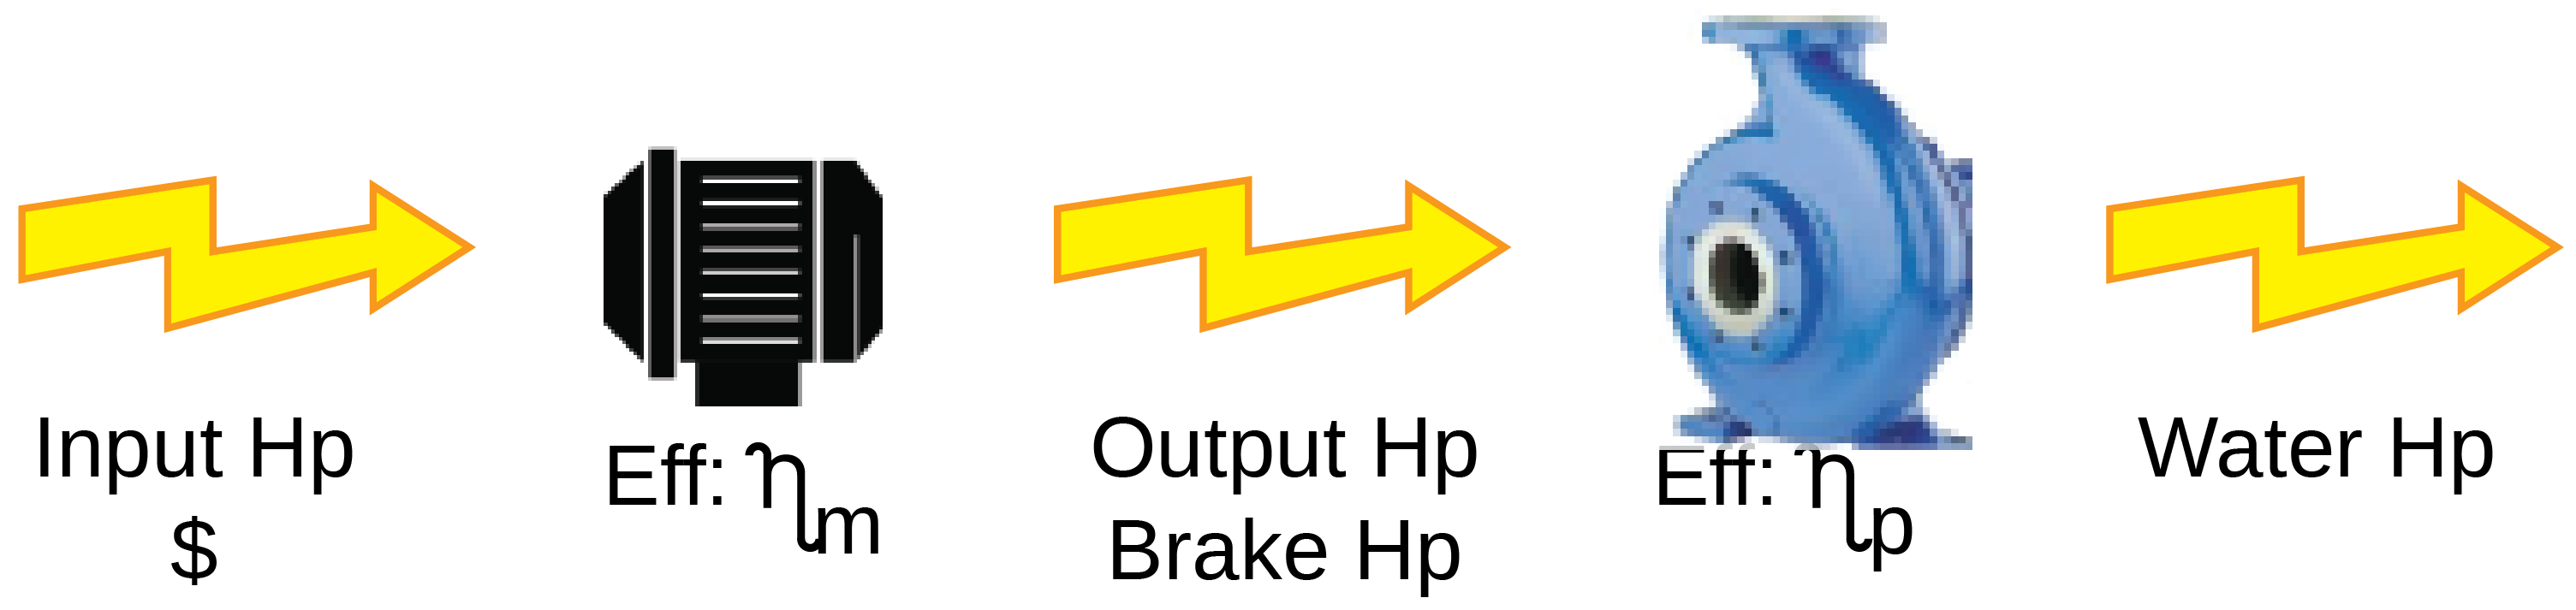
\includegraphics[scale=0.08]{PumpProblem}\\
 \vspace{0.2cm}
 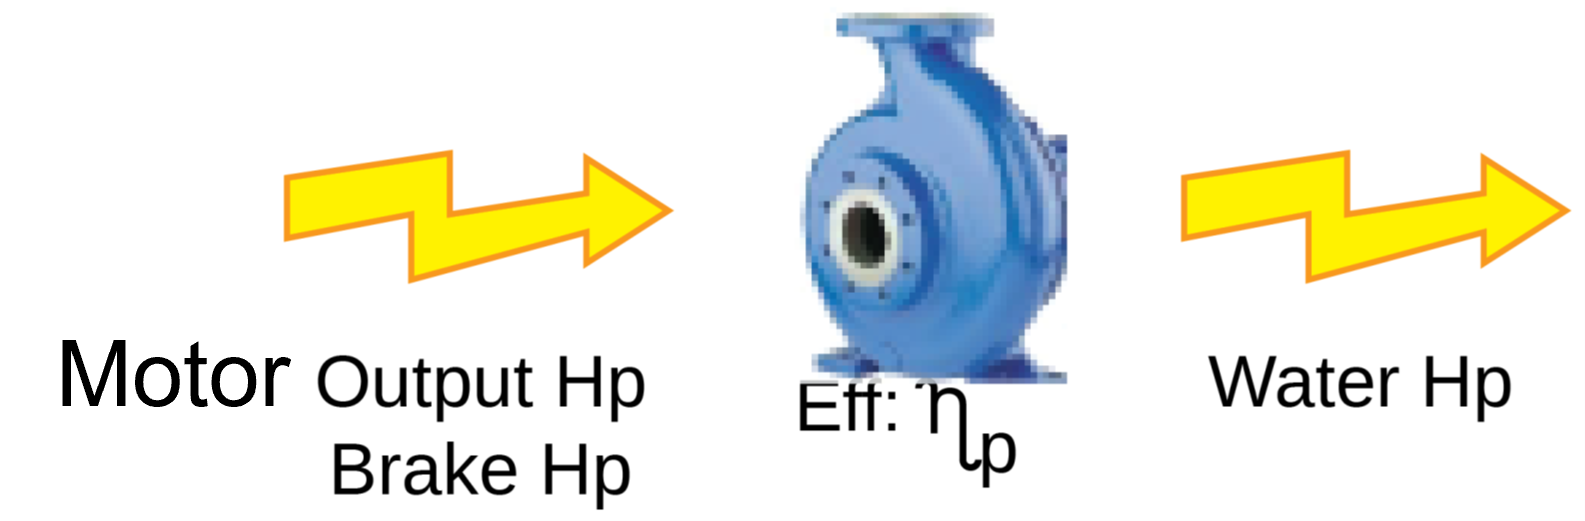
\includegraphics[scale=0.32]{PumpingProblemPump}
 $\eta_p=\dfrac{10 \mathrm{BHp}}{15.4 \mathrm{EHp}} \times 100=\boxed{65 \%}$
 \vspace{0.2cm}
 
 
 \item Solution:\\
  \vspace{0.2cm}
 \vspace{0.32cm}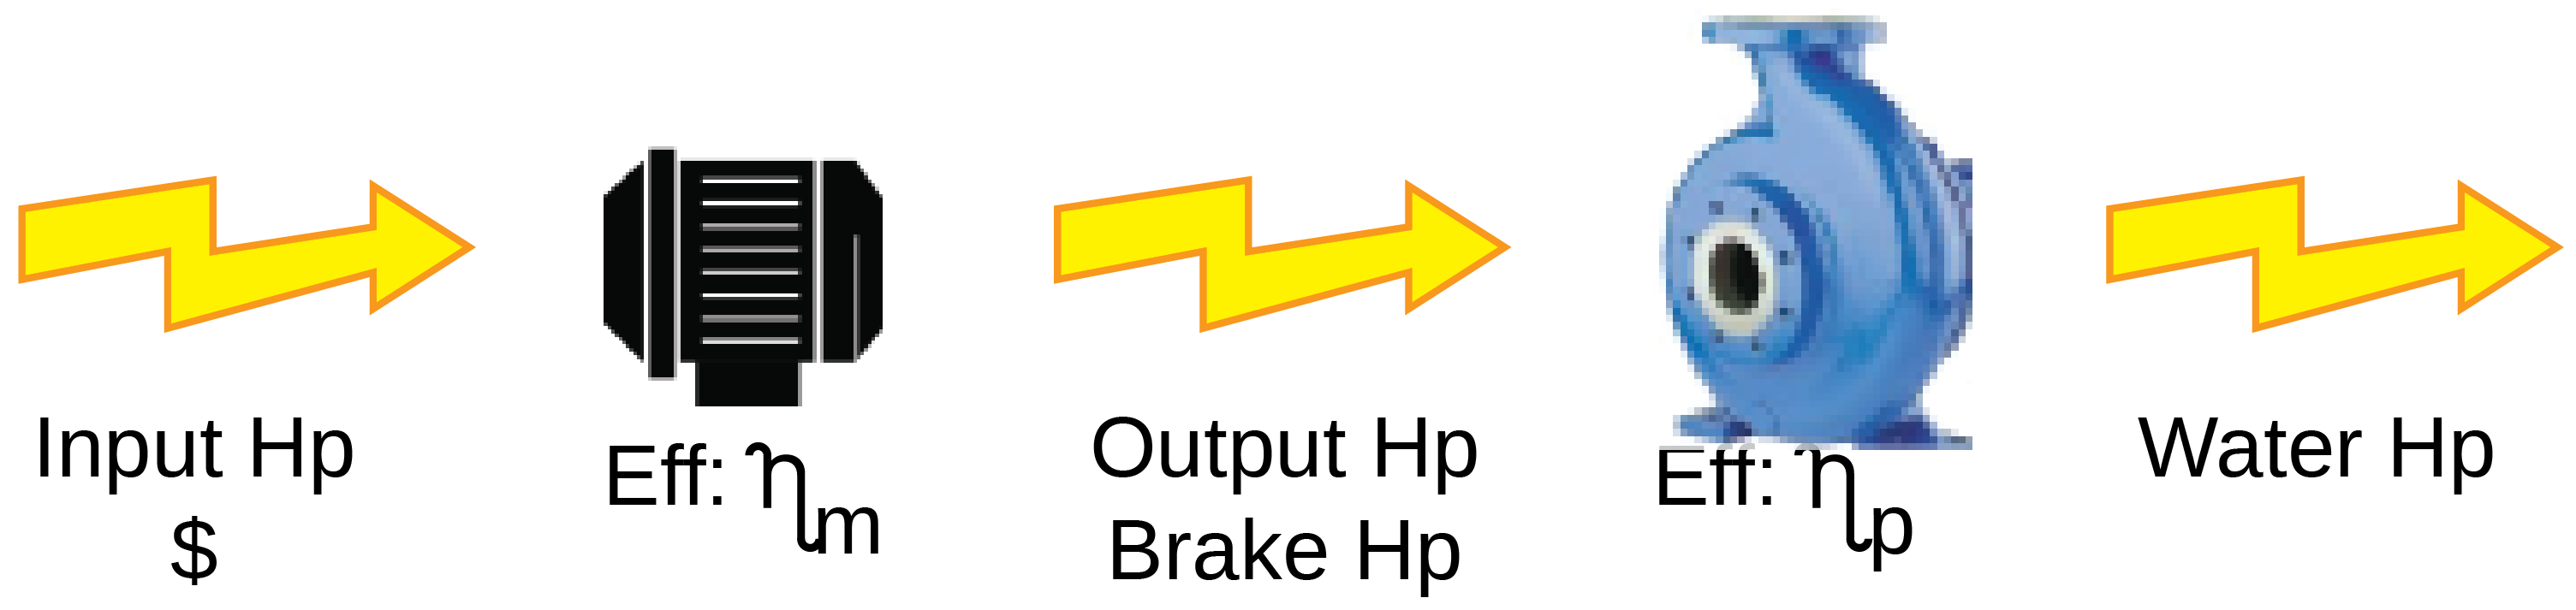
\includegraphics[scale=0.08]{PumpProblem}\\
 \vspace{0.2cm}
 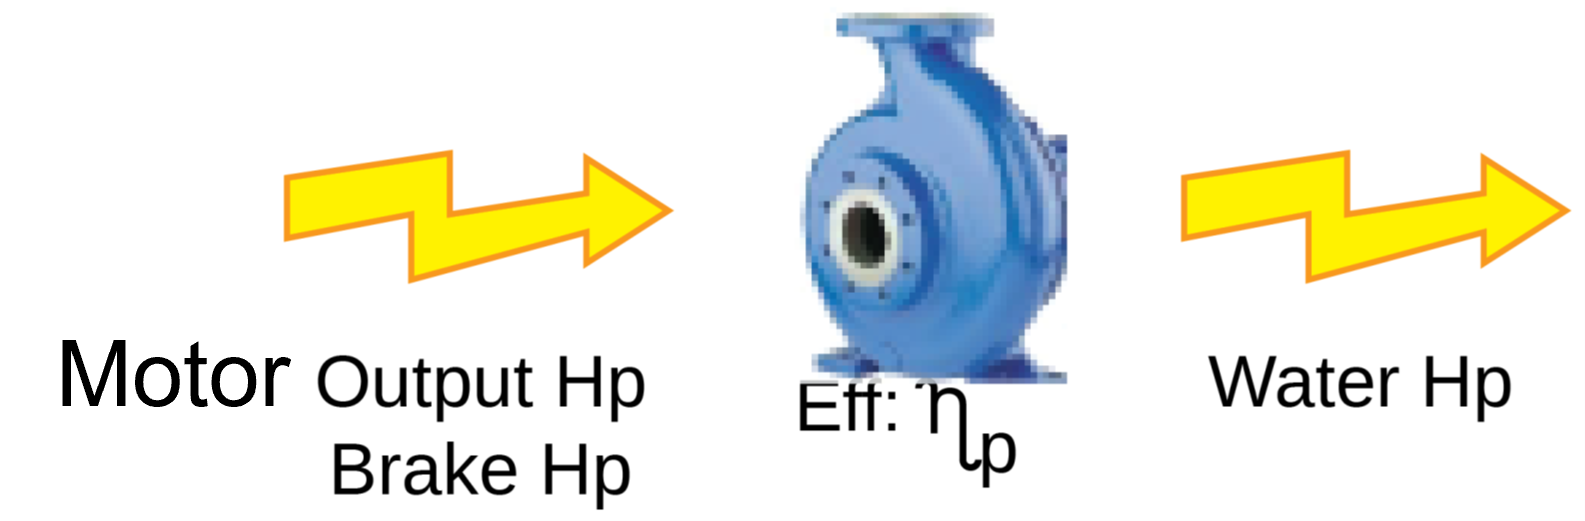
\includegraphics[scale=0.4]{PumpingProblemPump}
 \vspace{0.2cm}
$\eta_p=\dfrac{25 \mathrm{\enspace Water \enspace Hp}}{48 \mathrm{\enspace brake \enspace Hp}} \times 100=\boxed{52 \%}$
  \vspace{0.4cm}
 \item Solution:\\ 
 \vspace{0.2cm}
$Well \enspace efficiency=\eta_m * \eta_p \implies 0.94 \times 0.75=0.705 \times 100=\boxed{71 \%}$
 \vspace{0.2cm}


 \item Solution:\\
 \vspace{0.4cm}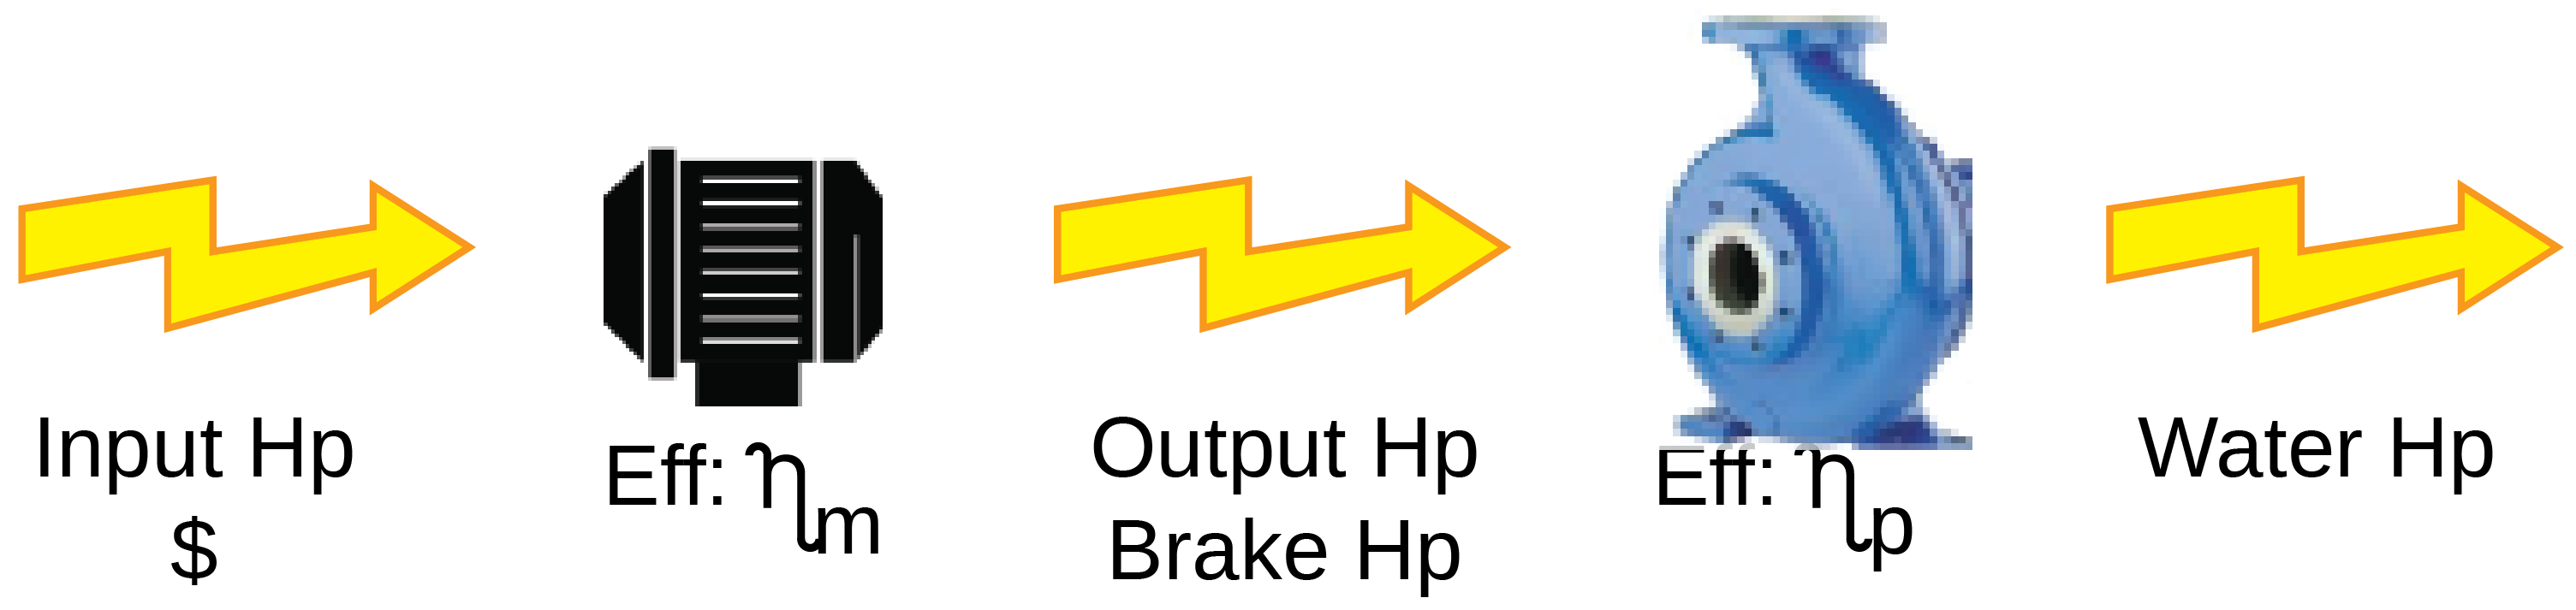
\includegraphics[scale=0.08]{PumpProblem}\\
 \vspace{0.2cm}
 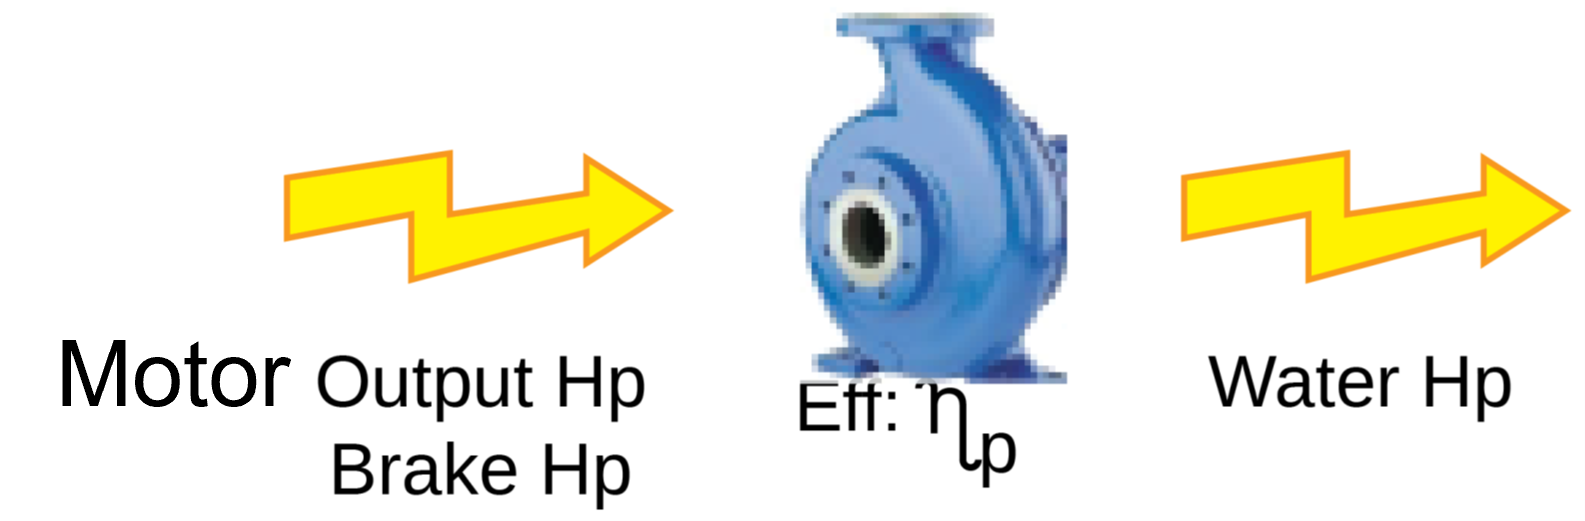
\includegraphics[scale=0.32]{PumpingProblemPump}
 \vspace{0.2cm}
$\dfrac{10 \mathrm{BHp}}{0.85}=\boxed{12 \mathrm{EHp \enspace or \enspace Input \enspace Hp}}$
 \vspace{0.4cm}


  \item Solution:\\ 
  \vspace{0.2cm}
 \vspace{0.08cm}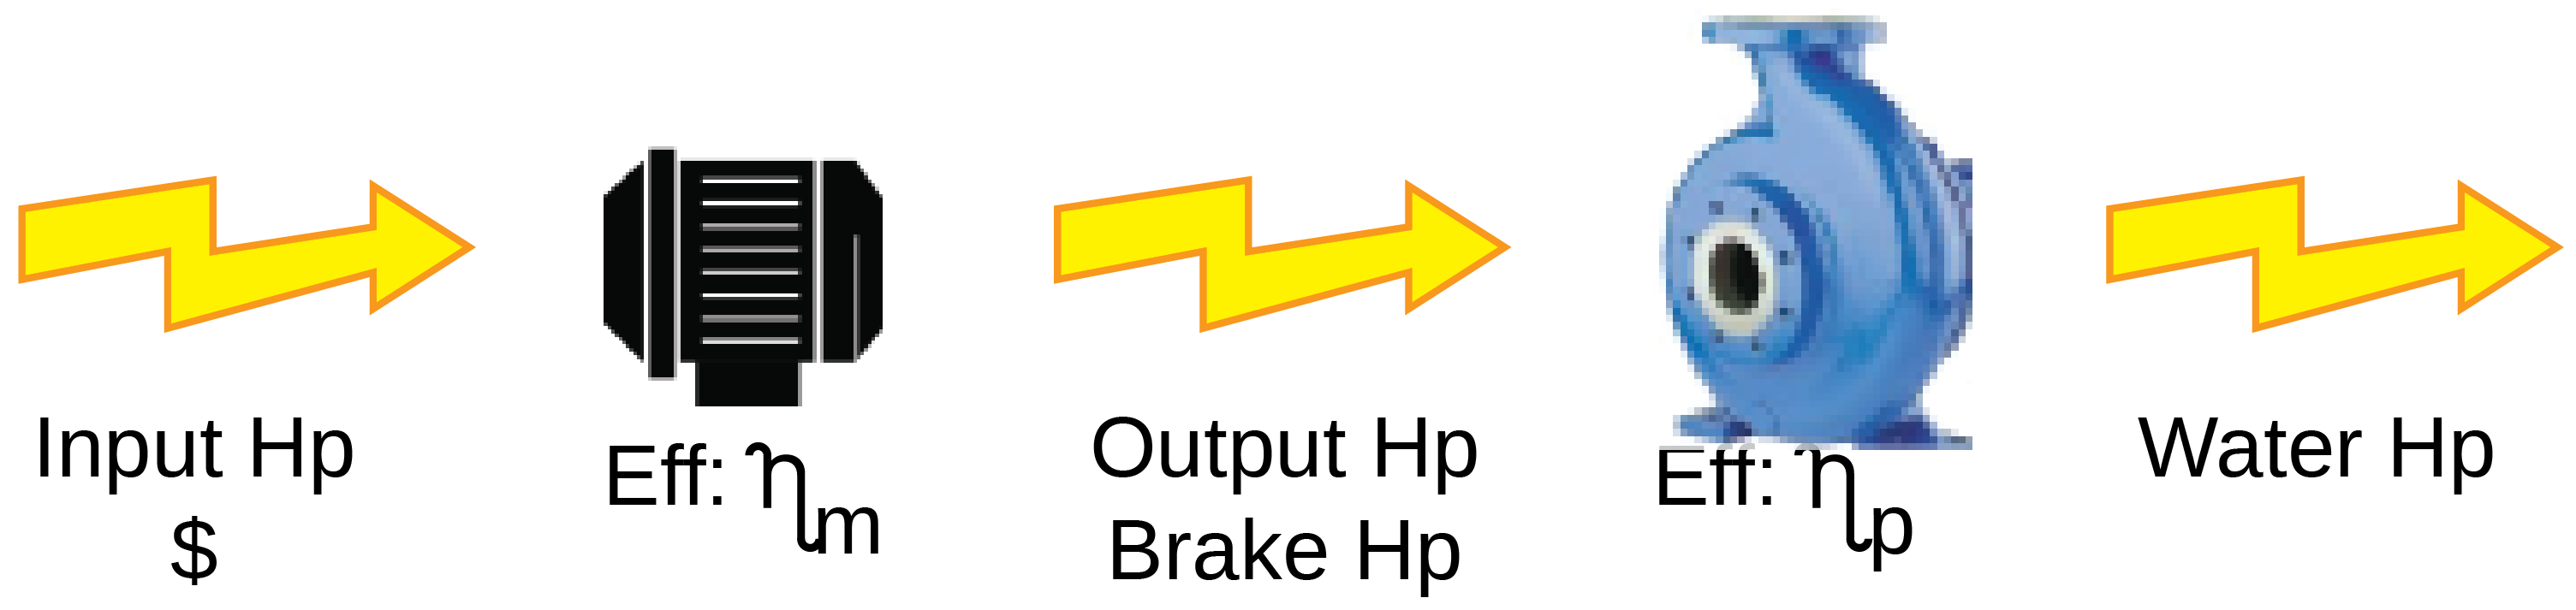
\includegraphics[scale=0.08]{PumpProblem}\\
 \vspace{0.2cm}
 \includegraphics[scale=0.32]{PumpingProblempump}
 \vspace{0.2cm}
$\eta_p=\dfrac{8.2 \mathrm{\enspace W \enspace Hp}}{10.3 \mathrm{\enspace BHp}} \times 100=\boxed{80 \%}$
 \vspace{0.2cm}


\item Solution:\\
\vspace{0.4cm}
water Hp = flow * head\\
\vspace{0.4cm}
$\mathrm{Water} \enspace \mathrm{Hp} = 120 \enspace \mathrm{gpm}*1,200 \enspace ft*\dfrac{\mathrm{Hp}}{3,960 \enspace \mathrm{gpm-ft}}=\boxed{ 37 \enspace \mathrm{Hp}}$\\
\vspace{0.2cm}


\item Solution:\\
\vspace{0.4cm}
$25 \enspace \mathrm{Hp}\dfrac{0.746 \enspace \mathrm{kW}}{\mathrm{Hp}}*\dfrac{8 \enspace \mathrm{hrs}}{\mathrm{day}}*\dfrac{7 \enspace \mathrm{days}}{\mathrm{month}}*\dfrac{\$0.07}{\mathrm{kWh}}=\boxed{\dfrac{\$73.1}{\mathrm{week}}}$\\
\vspace{0.2cm}

 \item Solution:\\
 \vspace{0.4cm}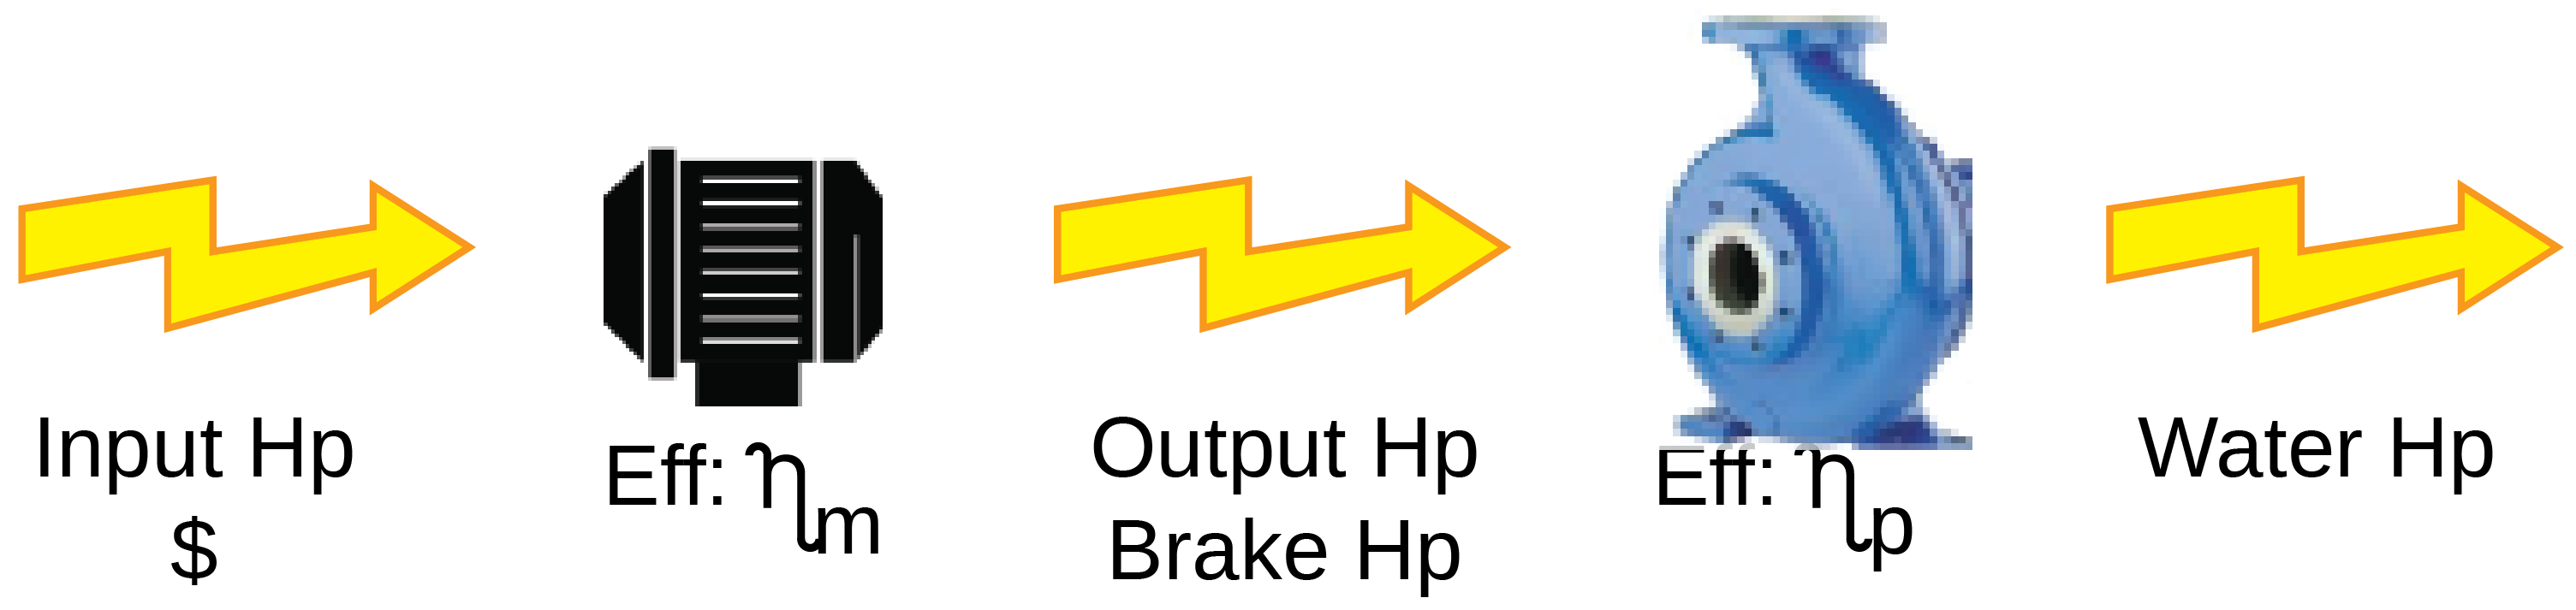
\includegraphics[scale=0.08]{PumpProblem}\\
 \vspace{0.2cm}
 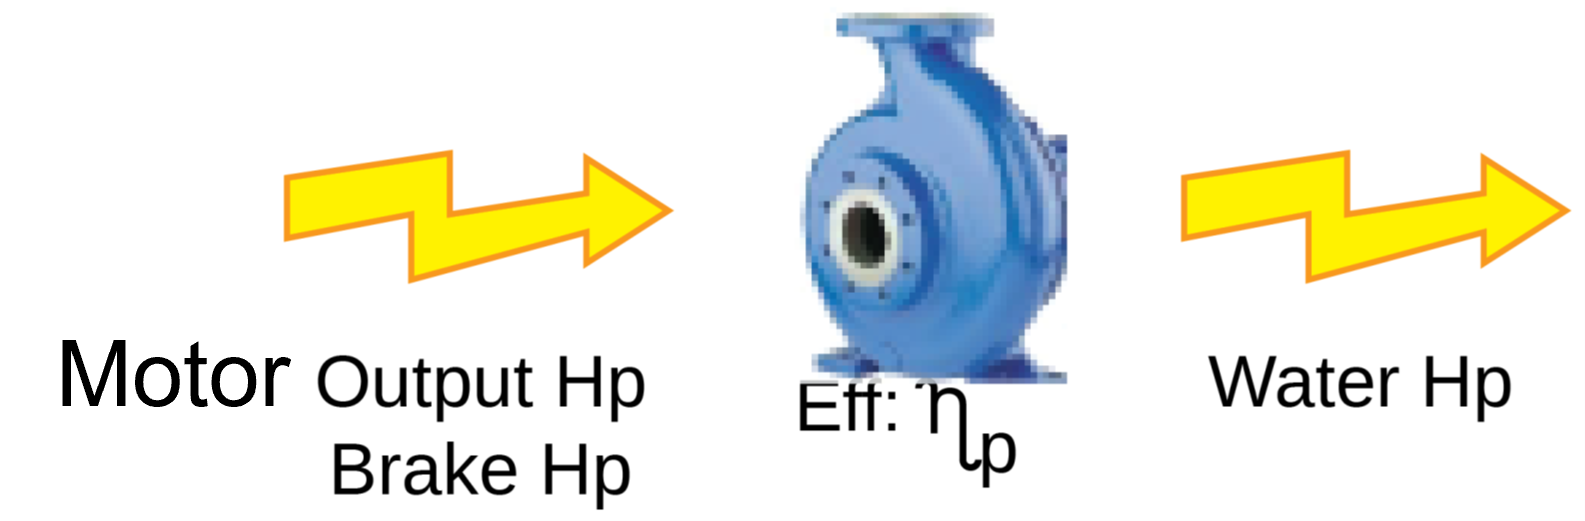
\includegraphics[scale=0.32]{PumpingProblemPump}
 \vspace{0.2cm}

water Hp = flow * head\\
 \vspace{0.2cm}
$\mathrm{Water} \enspace \mathrm{Hp} = 500 \enspace \mathrm{gpm}*50 \enspace ft*\dfrac{\mathrm{Hp}}{3,960 \enspace \mathrm{gpm-ft}}=\boxed{ 6.3 \enspace \mathrm{WHp}}$\\ 
  \vspace{0.2cm}
$\mathrm{Pump \enspace efficiency} =\dfrac{\mathrm{water \enspace Hp}}{\mathrm{brake \enspace Hp}} \implies \mathrm{brake \enspace Hp}=\dfrac{\mathrm{pump \enspace Hp}}{\mathrm{Pump \enspace efficiency}}$ \\
  \vspace{0.2cm}
$\textrm{brake} \enspace Hp = \dfrac{6.3}{0.85}=\boxed{7.4 \enspace \mathrm{Hp}}$\\
  \vspace{0.2cm}
$\mathrm{Motor \enspace efficiency} =\dfrac{\mathrm{brake \enspace Hp}}{\mathrm{input \enspace Hp}} \implies \mathrm{input \enspace \enspace Hp}=\dfrac{\mathrm{brake \enspace Hp}}{\mathrm{motor \enspace efficiency}}= \dfrac{7.4}{0.9}=\boxed{8.2 \enspace \mathrm{Hp}}$\\
  \vspace{0.2cm}
  
 \vspace{0.2cm}
$\mathrm{Wire-to-water} \enspace \mathrm{efficiency}=\eta_m * \eta_p \implies 0.9 \times 0.85 \times 100=\boxed{77 \%}$

\item  Solution:\\
\vspace{0.4cm}
water Hp = flow * head\\
$150 \enspace \mathrm{GPM}*75\mathrm{ft}*\dfrac{Hp}{3,960 GPM-ft}=\boxed{Water \enspace Hp = 2.8Hp}$\\
\vspace{0.4cm}
pump Hp = brake Hp * pump efficiency\\
$brake \enspace Hp = \dfrac{2.8}{0.9}=\boxed{Brake \enspace Hp=3.1Hp}$
 \vspace{0.2cm}

\end{enumerate}





